%
% skript.tex -- Skript ueber Klimawandel
%
% (c) 2017 Prof. Dr. Andreas Mueller, HSR
%
\documentclass{book}
\usepackage{etex}
\usepackage{geometry}
\geometry{papersize={170mm,240mm},total={140mm,200mm},top=21mm,bindingoffset=10mm}
\usepackage[english,ngerman]{babel}
\usepackage[utf8]{inputenc}
\usepackage[T1]{fontenc}
\usepackage{cancel}
\usepackage{times}
\usepackage{amsmath,amscd}
\usepackage{amssymb}
\usepackage{amsfonts}
\usepackage{amsthm}
\usepackage{graphicx}
\usepackage{fancyhdr}
\usepackage{textcomp}
\usepackage{txfonts}
%\usepackage{alltt} 
\newcommand\hmmax{0}
\newcommand\bmmax{0}
\usepackage{bm}
\usepackage{verbatim}
\usepackage{paralist}
\usepackage{makeidx}
\usepackage{array}
%\usepackage[colorlinks=true]{hyperref}
\usepackage{hyperref}
\usepackage{tikz}
\usepackage{pgfplots}
\usepackage{pgfplotstable}
\usepackage{pdftexcmds}
\usepackage{pgfmath}
%\usepackage{placeins}
%\usepackage{subfigure}
\usepackage[autostyle=false,english=american]{csquotes}
%\usepackage{float}
%\usepackage{enumitem}
\usepackage{wasysym}
\usepackage{environ}
%\usepackage{pifont}
%\usepackage{feynmp}
\usepackage{appendix}
\usetikzlibrary{calc,intersections,through,backgrounds,graphs,positioning,shapes,arrows,fit}
\usetikzlibrary{patterns,decorations.pathreplacing}
\usetikzlibrary{decorations.pathreplacing}
\usetikzlibrary{external}
\usetikzlibrary{datavisualization}
\usepackage[europeanvoltages,
            europeancurrents,
            europeanresistors,   % rectangular shape
            americaninductors,   % "4-bumbs" shape
            europeanports,       % rectangular logic ports
            siunitx,             % #1<#2>
            emptydiodes,
            noarrowmos,
            smartlabels]         % lables are rotated in a smart way
           {circuitikz}          %
\usepackage{siunitx}
\usepackage{tabularx}
\usetikzlibrary{arrows}

\usepackage{algpseudocode}
\usepackage{algorithm}
\usepackage{gensymb}
\usepackage{mathtools}


% Matlab
\usepackage{listings}
\usepackage{color} %red, green, blue, yellow, cyan, magenta, black, white
\definecolor{mygreen}{RGB}{28,172,0} % color values Red, Green, Blue
\definecolor{mylilas}{RGB}{170,55,241}

\lstset{language=Matlab,%
    %basicstyle=\color{red},
    breaklines=true,%
    morekeywords={matlab2tikz},
    keywordstyle=\color{blue},%
    morekeywords=[2]{1}, keywordstyle=[2]{\color{black}},
    identifierstyle=\color{black},%
    stringstyle=\color{mylilas},
    commentstyle=\color{mygreen},%
    showstringspaces=false,%without this there will be a symbol in the places where there is a space
    numbers=left,%
    %numberstyle={\tiny \color{black}},% size of the numbers
    numbersep=9pt, % this defines how far the numbers are from the text
    emph=[1]{break},emphstyle=[1]\color{red}, %some words to emphasise
    %emph=[2]{word1,word2}, emphstyle=[2]{style},    
}
\lstdefinestyle{Matlab}{
  numbers=left,
  belowcaptionskip=1\baselineskip,
  breaklines=true,
  frame=L,
  xleftmargin=\parindent,
  language=Matlab,
  showstringspaces=false,
  basicstyle=\footnotesize\ttfamily,
  keywordstyle=\bfseries\color{green!40!black},
  commentstyle=\itshape\color{purple!40!black},
  identifierstyle=\color{blue},
  stringstyle=\color{orange},
  numberstyle=\ttfamily\tiny
}
\lstdefinelanguage{Matlab}{
  keywords={function,global,size,zeros,switch,case,otherwise,end,sin,cos,cot,floor,ode45,hold,polarplot},
  sensitive=true
}
\lstdefinelanguage{Maxima}{
  keywords={addrow,addcol,zeromatrix,ident,augcoefmatrix,ratsubst,sum,diff,ev,tex,%
    with_stdout,nouns,express,depends,load,length,submatrix,div,grad,curl,matrix,%
    invert,lambda,facsum,expand,false,then,if,else,subst,batchload,%
    rootscontract,solve,part,assume,sqrt,integrate,abs,inf,exp,sin,cos,sinh,cosh,taylor,ratsimp},
  sensitive=true,
  comment=[n][\itshape]{/*}{*/}
}
\lstdefinestyle{Maxima}{
  numbers=left,
  belowcaptionskip=1\baselineskip,
  breaklines=true,
  frame=L,
  xleftmargin=\parindent,
  language=Maxima,
  showstringspaces=false,
  basicstyle=\footnotesize\ttfamily,
  keywordstyle=\bfseries\color{green!40!black},
  commentstyle=\itshape\color{purple!40!black},
  identifierstyle=\color{blue},
  stringstyle=\color{orange},
  numberstyle=\ttfamily\tiny
}
\lstset{language=Octave,%
    %basicstyle=\color{red},
    breaklines=true,%
    morekeywords={function,global,size,zeros,switch,case,otherwise,end,sin,cos,cot,floor,ode45,hold,polarplot,endfunction,size,endswitch,cat,printf,for,endfor,if,return,endif,abs,while,endwhile},
    keywordstyle=\color{blue},%
    morekeywords=[2]{1}, keywordstyle=[2]{\color{black}},
    identifierstyle=\color{black},%
    stringstyle=\color{mylilas},
    commentstyle=\color{mygreen},%
    showstringspaces=false,%without this there will be a symbol in the places where there is a space
    numbers=left,%
    %numberstyle={\tiny \color{black}},% size of the numbers
    numbersep=9pt, % this defines how far the numbers are from the text
    emph=[1]{break},emphstyle=[1]\color{red}, %some words to emphasise
    %emph=[2]{word1,word2}, emphstyle=[2]{style},    
}
\lstdefinestyle{Octave}{
  numbers=left,
  belowcaptionskip=1\baselineskip,
  breaklines=true,
  frame=L,
  xleftmargin=\parindent,
  language=Octave,
  showstringspaces=false,
  basicstyle=\footnotesize\ttfamily,
  keywordstyle=\bfseries\color{green!40!black},
  commentstyle=\itshape\color{purple!40!black},
  identifierstyle=\color{blue},
  stringstyle=\color{orange},
  numberstyle=\ttfamily\tiny
}
\lstdefinestyle{C}{
  numbers=left,
  belowcaptionskip=1\baselineskip,
  breaklines=true,
  frame=L,
  xleftmargin=\parindent,
  language=C,
  showstringspaces=false,
  basicstyle=\footnotesize\ttfamily,
  keywordstyle=\bfseries\color{green!40!black},
  commentstyle=\itshape\color{purple!40!black},
  identifierstyle=\color{blue},
  stringstyle=\color{orange},
  numberstyle=\ttfamily\tiny
}
\usepackage{caption}
\usepackage[mode=buildnew]{standalone}
\usepackage[backend=bibtex]{biblatex}

% additional packages
%
% packages.tex -- zusätzliche Packages 
%
% In diesem File werden \usepackage{}-Aufrufe eingetragen für Packages, die
% noch nicht im skript.tex aufgerufen werden
%
% (c) 2018 Michael Müller, Hochschule Rapperswil
%


%
% packages.tex -- zusätzliche Packages 
%
% In diesem File werden \usepackage{}-Aufrufe eingetragen für Packages, die
% noch nicht im skript.tex aufgerufen werden
%
% (c) 2018 Michael Müller, Hochschule Rapperswil
%


%
% packages.tex -- zusätzliche Packages 
%
% In diesem File werden \usepackage{}-Aufrufe eingetragen für Packages, die
% noch nicht im skript.tex aufgerufen werden
%
% (c) 2018 Michael Müller, Hochschule Rapperswil
%


%
% packages.tex -- zusätzliche Packages 
%
% In diesem File werden \usepackage{}-Aufrufe eingetragen für Packages, die
% noch nicht im skript.tex aufgerufen werden
%
% (c) 2018 Michael Müller, Hochschule Rapperswil
%


%
% packages.tex -- zusätzliche Packages 
%
% In diesem File werden \usepackage{}-Aufrufe eingetragen für Packages, die
% noch nicht im skript.tex aufgerufen werden
%
% (c) 2018 Michael Müller, Hochschule Rapperswil
%


%
% packages.tex -- zusätzliche Packages 
%
% In diesem File werden \usepackage{}-Aufrufe eingetragen für Packages, die
% noch nicht im skript.tex aufgerufen werden
%
% (c) 2018 Michael Müller, Hochschule Rapperswil
%


%
% packages.tex -- zusätzliche Packages 
%
% In diesem File werden \usepackage{}-Aufrufe eingetragen für Packages, die
% noch nicht im skript.tex aufgerufen werden
%
% (c) 2018 Michael Müller, Hochschule Rapperswil
%


%
% packages.tex -- zusätzliche Packages 
%
% In diesem File werden \usepackage{}-Aufrufe eingetragen für Packages, die
% noch nicht im skript.tex aufgerufen werden
%
% (c) 2018 Michael Müller, Hochschule Rapperswil
%


%
% packages.tex -- zusätzliche Packages 
%
% In diesem File werden \usepackage{}-Aufrufe eingetragen für Packages, die
% noch nicht im skript.tex aufgerufen werden
%
% (c) 2018 Michael Müller, Hochschule Rapperswil
%


%
% packages.tex -- zusätzliche Packages 
%
% In diesem File werden \usepackage{}-Aufrufe eingetragen für Packages, die
% noch nicht im skript.tex aufgerufen werden
%
% (c) 2018 Michael Müller, Hochschule Rapperswil
%



% workaround for biblatex bug
\makeatletter
\def\blx@maxline{77}
\makeatother
\addbibresource{references.bib}
% Bibresources für jeden einzelnen Artikel
%\addbibresource{eis/references.bib}
%\addbibresource{extrem/references.bib}
%\addbibresource{kalman/references.bib}
%\addbibresource{learning/references.bib}
%\addbibresource{lorenz/references.bib}
%\addbibresource{lorenz2/references.bib}
%\addbibresource{planeten/references.bib}
%\addbibresource{thermohalin/references.bib}
%\addbibresource{vegetation/references.bib}
%\addbibresource{verzoegert/references.bib}
\AtEndDocument{\clearpage\ifodd\value{page}\else\null\clearpage\fi}
\makeindex
%\pgfplotsset{compat=1.12}
\setlength{\headheight}{15pt} % fix headheight warning
\DeclareGraphicsRule{*}{mps}{*}{}
\begin{document}
\pagestyle{fancy}
\frontmatter
\newcommand\HRule{\noindent\rule{\linewidth}{1.5pt}}
\begin{titlepage}
\vspace*{\stretch{1}}
\HRule
\vspace*{5pt}
\begin{flushright}
{
\LARGE
Mathematisches Seminar\\
\vspace*{20pt}
\Huge
Klimawandel%
}
\vspace*{5pt}
\end{flushright}
\HRule
\begin{flushright}
\vspace{60pt}
\Large
Leitung: Andreas Müller\\
\vspace{40pt}
\Large
%
% teilnehmer.tex -- Liste der Seminarteilnehmer für Titelseite
%
% (c) 2018 Prof Dr Andreas Müller, Hochschule Rapperswil
%
Matthias Baumann,
Oliver Dias-Lalcaca,
%Matthias Dunkel%,
Jonas Gründler%,
\\
Sebastian Lenhard,
Silvio Marti,
Michael~Müller,
Hansruedi~Patzen%,
\\
Melina~Staub,
Martin~Stypinski,
Nicolas Tobler,
Raphael Unterer
\\

\end{flushright}
\vspace*{\stretch{2}}
\begin{center}
Hochschule für Technik, Rapperswil, 2018
\end{center}
\end{titlepage}
\hypersetup{
    linktoc=all,
    linkcolor=blue
}
\newcounter{beispiel}
\newenvironment{beispiele}{
\bgroup\smallskip\parindent0pt\bf Beispiele\egroup

\begin{list}{\arabic{beispiel}.}
  {\usecounter{beispiel}
  \setlength{\labelsep}{5mm}
  \setlength{\rightmargin}{0pt}
}}{\end{list}}
\newcounter{uebungsaufgabezaehler}
% environment fuer uebungsaufgaben
\newenvironment{uebungsaufgaben}{
\begin{list}{\arabic{uebungsaufgabezaehler}.}
  {\usecounter{uebungsaufgabezaehler}
  \setlength{\labelwidth}{2cm}
  \setlength{\leftmargin}{0pt}
  \setlength{\labelsep}{5mm}
  \setlength{\rightmargin}{0pt}
  \setlength{\itemindent}{0pt}
}}{\end{list}\vfill\pagebreak}
\newenvironment{teilaufgaben}{
\begin{enumerate}
\renewcommand{\labelenumi}{\alph{enumi})}
}{\end{enumerate}}
% Aufgabe
\newcounter{problemcounter}[chapter]
\def\aufgabenpath{chapters/uebungsaufgaben/}
\def\ainput#1{\input\aufgabenpath/#1}
\def\verbatimainput#1{\expandafter\verbatiminput{\aufgabenpath/#1}}
\def\aufgabetoplevel#1{%
\expandafter\def\expandafter\inputpath{#1}%
\let\aufgabepath=\inputpath
}
\def\includeagraphics[#1]#2{\expandafter\includegraphics[#1]{\aufgabepath#2}}
% \aufgabe
\newcommand{\uebungsaufgabe}[1]{%
\refstepcounter{problemcounter}%
\label{#1}%
\bigskip{\parindent0pt\strut}\hbox{\bf\arabic{problemcounter}. }%
\expandafter\def\csname aufgabenpath\endcsname{\inputpath/}%
\expandafter\input{chapters/uebungsaufgaben/#1.tex}
}
\renewcommand\theproblemcounter{\thechapter.\arabic{problemcounter}}

% Loesung
\def\swallow#1{
%nothing
}
\NewEnviron{loesung}[1][Lösung]{%
\begin{proof}[#1]%
\renewcommand{\qedsymbol}{$\bigcirc$}
\BODY
\end{proof}
}
\NewEnviron{bewertung}{%
\begin{proof}[Bewertung]%
\renewcommand{\qedsymbol}{}
\BODY
\end{proof}
}
\NewEnviron{diskussion}{%
\begin{proof}[Diskussion]%
\renewcommand{\qedsymbol}{}
\BODY
\end{proof}
}
\NewEnviron{hinweis}{%
\begin{proof}[Hinweis]%
\renewcommand{\qedsymbol}{}
\BODY
\end{proof}
}
\def\keineloesungen{%
\RenewEnviron{loesung}{\relax}
\RenewEnviron{bewertung}{\relax}
\RenewEnviron{diskussion}{\relax}
}
\newenvironment{beispiel}{%
\begin{proof}[Beispiel]%
\renewcommand{\qedsymbol}{$\bigcirc$}
}{\end{proof}}

\allowdisplaybreaks

\lhead{Inhaltsverzeichnis}
\rhead{}
\tableofcontents
\newtheorem{satz}{Satz}[chapter]
\newtheorem{hilfssatz}[satz]{Hilfssatz}
\newtheorem{definition}[satz]{Definition}
\newtheorem{annahme}[satz]{Annahme}
\newtheorem{problem}[satz]{Problem}
\newtheorem*{problem*}{Problem}
\renewcommand{\floatpagefraction}{0.7}
\mainmatter
%
% vorwort.tex -- Vorwort zum Buch zum Seminar
%
% (c) 2017 Prof Dr Andreas Mueller, Hochschule Rapperswil
%
\chapter*{Vorwort}
\lhead{Vorwort}
\rhead{}
Dieses Buch entstand im Rahmen des Mathematischen Seminars
im Frühjahrssemester 2017 an der Hochschule für Technik Rapperswil.
Die Teilnehmer, Studierende der Abteilungen für Elektrotechnik,
Informatik und Bauingenieurwesen der
HSR, erarbeiteten nach einer Einführung in das Themengebiet jeweils
einzelne Aspekte des Gebietes in Form einer Seminararbeit, über
deren Resultate sie auch in einem Vortrag informierten. 

Im Frühjahr 2018 war das Thema des Seminars der Klimawandel.

Im zweiten Teil dieses Skripts kommen dann die Teilnehmer selbst zu Wort.
Ihre Arbeiten wurden jeweils als einzelne
Kapitel mit meist nur typographischen Änderungen übernommen.
Diese weiterführenden Kapitel sind sehr verschiedenartig.
Eine Übersicht und Einführung findet sich in der Einleitung
zum zweiten Teil auf Seite~\pageref{skript:uebersicht}.

In einigen Arbeiten wurde auch Code zur Demonstration der 
besprochenen Methoden und Resultate geschrieben, soweit
möglich und sinnvoll wurde dieser Code im Github-Repository
dieses Kurses%
\footnote{\url{https://github.com/AndreasFMueller/SeminarKlima.git}}
abgelegt.

Im genannten Repository findet sich auch der Source-Code dieses
Skriptes, es wird hier unter einer Creative Commons Lizenz
zur Verfügung gestellt.
Auf der beiliegenden DVD befinden sich die Testdaten und Programme
zu zwei der simulationsintensiveren Artikel im zweiten Teil.



\part{Grundlagen}
%\keineloesungen
\begin{refsection}
%
% part1.tex
%
% (c) 2018 Prof Dr Andreas Müller, Hochschule Rapperswil
%
%
% wuk.tex -- Wetter und Klima
%
% Einleitungskapitel, welches das Wetter- und Klimasystem der Erde in
% qualitiativer Form beschreibt
%
% (c) 2018 Prof Dr Andreas Müller, Hochschule Rapperswil
%
\chapter{Wetter und Klima\label{chapter:wetter und klima}}
\lhead{Wetter und Klima}
US Präsident Donald Trump war schon immer ein Klimaverweigerer, wie Tweets
aus der Zeit lange bevor er Präsident wurde:
\begin{center}

\includegraphics[width=\hsize]{chapters/1/trump.png}
\end{center}
Ganz offensichtlich versteht Trump den Unterschied zwischen Wetter und
Klima nicht.
Ziel dieses Kapitels ist, den Unterschied zwischen Wetter und Klima
zu klären.
Es ist allgemein bekannt, dass auch die besten Wetterprognosen im
günstigsten Fall für einige Tage zutreffen.
Daher soll in diesem Kapitel auch gezeigt werden, warm trotz dieser
Schwierigkeit das Klima sehr wohl langfristig modelliert und prognostiziert
werden kann.
Aus diesen Überlegungen wird auch klar, auf welche Aspekte des Klimasystems
sich ein Klima-Modell fokusieren muss, wenn eine langfristige Prognose
ermöglicht werden soll.

%
% klima.tex -- Klima
%
% (c) 2018 Prof Dr Andreas Müller, Hochschule Rapperswil
%

\section{Klima\label{section:klima}}
\rhead{Klima}
In der Wikipedia kann man die folgenden Definitionen für die Begriffe Wetter
und Klima finden:

\begin{definition}
Als {\em Wetter} bezeichnet man den
spürbaren, kurzfristigen Zustand der Atmosphäre (auch: messbarer
Zustand der Troposphäre) an einem bestimmten Ort der Erdoberfläche,
der unter anderem als Sonnenschein, Bewölkung, Regen, Wind, Hitze
oder Kälte in Erscheinung tritt
\cite{skript:wetter}.
\end{definition}

\begin{definition}
Das {\em Klima} steht als Begriff für die Gesamtheit aller meteorologischen
Vorgänge, die für die über Zeiträume von mindestens 30 Jahren
regelmässig wiederkehrenden durchschnittlichen Zustände der Erdatmosphäre
an einem Ort verantwortlich sind
\cite{skript:klima}.
\end{definition}

Was also Donald Trump in seinem Tweet beschrieben hat ist das Wetter.
Selbst wenn die Temperatur in New York unter den Gefrierpunkt fällt, 
heisst das nicht, dass die mittlere Temperatur in New York über mehrere
Jahre nicht doch ansteigen kann.
Tatsächlich bedeutet ``globale Erwärmung'' nicht, dass die mittlere
Temperatur an jedem Punkt der Erde zunehmen wird.
Im Gegenteil ist es durchaus möglich, dass zwar die mittlere Temperatur
der Erde ständig zunimmt, wie wir in den letzten Jahren auch messtechnisch
nachweisen konnten, dass aber auch die Temperaturunterschiede stark zunehmen,
so dass es am Ende an einzelnen Stelle der Erdoberfläche zu einer 
Abkühlung kommen kann.
Um dieser Komplexität Rechnung zu tragen, spricht man nicht mehr von
der ``globalen Erwärmung'', sondern vom Klimawandel.

Auch wenn das Wetter nur sehr eingeschränkt vorhersagen lässt,
bedeutet das noch lange nicht, dass das Klima nicht doch sehr
genau vorhergesagt werden kann.
Eine Analogie kann den Unterschied zwischen der Vorhersagbarkeit
von Wetter und Klima verdeutlichen.
Wenn man in einem Kochtopf Wasser zum Kochen bringt, stellt sich
eine unverrhersagbare chaotische Bewegung kleiner und grosser
Gasblasen ein.
Es ist unmöglich vorherzusagen, wann und wo sich die nächste Blase
bilden wird und welchen Weg sie an die Oberfläche des Wasser nehmen
wird.
Wenn wir aber nur die mittlere Temperatur betrachten, können wir
aus der Heizleistung der Kochplatte, der Masse und der spezifischen
Wärmekapazität des Wassers genau berechnen, welche Temperatur zu welcher
Zeit im Wasser herschen wird und wir können den Zeitpunkt exakt
vorhersagen, wann das Wasser zu sieden beginnt.
Die mittlere Temperatur des Wassers beschreibt das ``Klima''
in der Pfanne, die kleinräumigen und kurzfristigen Blasen und anderen
Turbulenzen beschreiben das ``Wetter''.


%
% physik.tex -- Physikalische Eigenschaften des Klimasystems
%
% (c) 2018 Prof Dr Andreas Müller, Hochschule Rapperswil
%

\section{Physikalische Eigenschaften des Klimasystems\label{section:physik}}
\rhead{Physikalische Eigenschaften des Klimasystems}
In diesem Abschnitt stellen wir die physikalischen Eigenschaften
aller wesentlichen Komponenten des Klimasystems zusammen.
Dabei geht es zunächst nur darum, die grundlegende Physik in 
Erinnerung zu rufen und die Naturgesetze, die die Wechselwirkungen
zwischen den Komponenten beschreiben.
Auf die Details der mathematischen Modellierung der zukünftigen
Veränderung dieser Grössen werden wir erst später eingehen.

\subsection{Wärme, Konvektion, Kondensation}
Die wohl wichtigste Klima-Grösse ist die Temperatur.
Sie drückt aus, wieviel Energie in Form von Wärme ein Körper oder eine
Komponente des Klimasystems enthält.

\subsubsection{Wärmekapazität}
Die spezifische Wärme $C$ gibt an, wie die innere Energie $U$ sich bei
einer Temperaturänderung $\Delta T$ verändert:
\[
\Delta U = C\cdot\Delta T.
\]
Der Körper speichert Energie in Form der thermischen Bewegung der
einzelnen Atome.
Schwerere Atome können bei gleicher Bewegungsgeschwindigkeit 
mehr Energie speichern.
Stoffe mit grösserer Dichte können mehr Atome und damit auch mehr
Wärmeenergie in einem kleineren Volumen unterbringen.
Die spezifische Wärmekapazität $c$ gibt an, welche Wärmekapazität
ein Kilogramm eines Stoffes hat.
Ein Körper der Masse $m$ hat also die Wärmekapazität $C=c\cdot m$.

\subsubsection{Wärmeleitung\label{subsection:heatconduction}}
Herrschen in einem Körper Temperaturunterschiede, ist $T$ nicht mehr
nur eine Konstante sondern eine Funktion $T(x,y,z,t)$
der Koordinaten und auch der Zeit.
Temperaturunterschiede werden sich ausgleichen, indem Energie von
wärmeren zu kälteren Teilen des Körpers fliegt.
Dies geschieht umso schneller, je grösser die Unterschiede sind.
Die Wärmeleitungsgleichung
\begin{equation}
\frac{\partial T}{\partial t}
=
\kappa
\biggl(
\frac{\partial^2}{\partial x^2}
+
\frac{\partial^2}{\partial y^2}
+
\frac{\partial^2}{\partial z^2}
\biggr)
T
\label{skript:waermeleitung}
\end{equation}
beschreibt die Entwicklung der Funktion $T(x,y,z,t)$ an jedem
Ort des Raumes \cite{skript:waermeleitung}.
Der Koeffizient $\kappa$ ist eine Materialkonstante, die beschreibt,
wie schnell sich die Temperaturunterschiede ausgleichen können.
Ist $\kappa=0$, folgt $\partial T/\partial t=0$, die Temperatur 
ändert sich nicht, es findet keine Wärmeleitung statt.

Die rechte Seite von \eqref{skript:waermeleitung} kann mit dem
sogenannten Laplace-Operator gemäss der folgenden Definition 
geschrieben werden.

\begin{definition}
Der Operator
\[
\Delta
=
\frac{\partial^2}{\partial x^2}
+
\frac{\partial^2}{\partial y^2}
+
\frac{\partial^2}{\partial z^2}
\]
heisst der
{\em Laplace-Operator}.
\end{definition}

Die Wärmeleitungsgleichung erhält damit die Form
\begin{equation}
\frac{\partial T}{\partial t}
=
\kappa\Delta T.
\label{skript:waermeleitung2}
\end{equation}
In einer Dimension wird daraus
\[
\frac{\partial T}{\partial t} = \kappa \frac{\partial^2 T}{\partial x^2}.
\]
Die Änderung der Temperatur ist also umso grösser, je grösser
die Krümmung der Temperaturkurve $x\mapsto T(x,t)$ ist.
Die Wärmeleitungsgleichung beschreibt also, wie sich die Temperaturen
ausgleichen, bis nur noch lineare Temperaturgradienten bestehen bleiben.

\subsubsection{Randbedingungen}
Die partielle Differentialgleichung~\eqref{skript:waermeleitung2}
alleine legt die Temperaturverteilung noch nicht fest.
Vielmehr muss man ausserdem die Temperatur zur willkürlich als $t=0$
gewählten Anfangszeit kennen, und die Temperatur am Rand des
Definitionsgebietes.
Erst zusammen mit diesen Randbedingungen ist die Lösung eindeutig festgelegt.

\subsubsection{Konvektion}
Wärmeleitung kann Wärmeenergie nur vergleichsweise langsam transportieren.
Das einleitende Beispiel des Kochtopfs zeigt auch, wie ein effizienterer
Energietransport funktionieren kann.
In der Atmosphäre dehnt sich warme Luft aus.
Dank der geringeren Dichte können warme Luftblasen aufsteigen und damit
Wärme viel effizienter in die obere Atmosphäre transportieren
als dies mit Wärmeleitung möglich wäre.
Dieser Prozess heisst {\em Konvektion} \cite{skript:konvektion}.
\index{Konvektion}%

\subsubsection{Advektion}
Wir wollen den Fall eines strömenden Mediums mathematisch etwas genauer
ausarbeiten.
Bewegt sich das Medium mit der Geschwindigkeit $\vec v$, dann ändert sich
die Temperatur des Mediums, welches sich über dem Punkt $P=(x,y,z)$
befindet.
Nach der Zeit $\Delta t$ befindet sich derjenige Teil des Mediums
über dem Punkt $P$, der sich vorher über dem Punkt $P-\Delta t\cdot\vec v$
befand.
Die Temperatur zur Zeit $t+\Delta t$ ist daher
$T(P,t+\Delta t)=T(P-\vec{v}\,\Delta t,t)$.
Die Temperaturänderung ist
\begin{align*}
T(P,t+\Delta t)
&=
T(P,t) + (T(P,t+\Delta t)-T(P,t))
=
T(P,t) + T(P-\vec v\,\Delta t, t)-T(P,t)
\\
\intertext{und damit die Temperaturänderung pro Zeiteinheit}
\frac{
T(P,t+\Delta t)
-
T(P,t)
}{\Delta t}
&=
\frac{
T(P-\vec{v}\,\Delta t, t)-T(P,t)
}{\Delta t}.
\end{align*}
Beim Grenzübergang $\Delta t\to 0$ wird aus der linken Seite die
partielle Ableitung nach $t$.
Die rechte Seite kann mit Hilfe der Kettenregel berechnet weren.
Es wird
\begin{equation}
\frac{\partial T}{\partial t}
=
-
\frac{\partial T}{\partial x} v_x
-
\frac{\partial T}{\partial y} v_y
-
\frac{\partial T}{\partial z} v_z.
\label{skript:advektion1}
\end{equation}
Der Ausdruck auf der rechten Seite kann vektoriell mit der folgenden
Definition etwas eleganter geschrieben werden.

\begin{definition}
Der vektorielle Operator 
\[
\nabla
=
\def\arraystretch{1.3}
\begin{pmatrix}
\frac{\partial}{\partial x}\\
\frac{\partial}{\partial y}\\
\frac{\partial}{\partial z}
\end{pmatrix}
\]
heisst der {\em Nabla-Operator}.
Der Vektor
\[
\nabla f
=
\def\arraystretch{1.3}
\begin{pmatrix}
\frac{\partial f}{\partial x}\\
\frac{\partial f}{\partial y}\\
\frac{\partial f}{\partial z}
\end{pmatrix}
=
\operatorname{grad} f
\]
heisst der {\em Gradient} von $f$.
Das Skalarprodukt $\nabla\cdot\vec{v}$ ist ein Skalar, die
{\em Divergenz}
eines Vektorfeldes $\vec{v}$, sie wird manchmal auch
$\operatorname{div}\vec{v}$ geschrieben.
\end{definition}
\index{Gradient}%
\index{Divergenz}%
\index{Nabla-Operator}%

Die Temperaturänderung in Folge der Strömung 
\eqref{skript:advektion1}
wird 
\begin{equation}
\frac{\partial T}{\partial t}
=
-\vec{v}\cdot\nabla T.
\label{skript:advektion2}
\end{equation}
\index{Advektion}%
Man nennt diese Temperaturänderung durch die Strömung auch
{\em Advektion}.
Die Wärmeleitungsgleichung kann damit zu einem umfassenderen
Modell
\begin{equation}
\frac{\partial T}{\partial t}
=
-\vec{v}\cdot\nabla T +\kappa\Delta T
\label{skript:waermeleitungadvektion}
\end{equation}
zusammengefasst werden.
Es ist geeignet für die Beschreibung sowohl der Atmosphäre wie auch des
Wärmeaustausches in den Ozeanen.

\subsubsection{Phasenübergänge}
Um ein Kilogramm Wasser bei $20^\circ\text{C}$ zu verdunsten, ist eine
latente Wärme von $2480\,\text{kJ}$ nötig.
\index{latente Wärme}%
Um ein Kilogramm Luft um ein Grad zu erwärmen, sind dagegen nur
$1.005\,\text{kJ}$ notwendig.
Anders herum bedeutet dies, dass eine mit Wasserdampf angereicherte Atmosphäre
sehr viel mehr Energie in Form von latenter Wärme speichern kann, als
allein durch die Wärmekapazität trockener Luft möglich wäre.
\index{latente Wärme}%

Wir haben damit zwei Mechanismen identifiziert, wie eingestrahlte
und in der Erdkruste als Wärme gespeicherte Energie in die Atmosphäre 
transportiert werden kann.
Einerseits kann Luft über aufgewärmten Landmassen oder dem Meer erwärmt
werden und als Konvektionsströmung aufsteigen.
Andererseits kann Wasser an der Oberfläche verdampft werden und damit die
latente Wärme in die Atmosphäre übergehen.
Man nennt diese Mechanismen auch turbulente Flüsse
\cite[S.~70]{skript:wiefunktioniertdas}.
\index{turbulente Flüsse}%

Der Wassergehalt der Luft kann höchstens einige wenige Prozente betragen.
Zwar ist die Wärmespeicherung durch Verdunstung über 2000 mal effizienter,
aber weil nur wenig Wasser dafür zur Verfügung steht, übernimmt die Verdunstung
doch nicht einen derart grossen Teil des Energietransports von der
Oberfläche in die Atmosphäre.
In der Tat finden etwa 30\% des Energietransports von der Erdkruste
in die Atmosphäre durch turbulente Flüsse statt, davon etwa
7\% durch Konvektion und 23\% durch latente Wärme
\cite[S.~70]{skript:wiefunktioniertdas}.
Höhere Temperaturen begünstigen die Verdunstung und verschieben diesen
Anteil zugunsten der latenten Wärme.
Man darf also davon ausgehen, dass höhere Oberflächentemperaturen
zu einem überproportional höheren Energietransport in die Atmosphäre
führen.

In der Atmosphäre kann die Energie über grosse Distanzen transportiert
und später wieder freigesetzt werden, wie Hurricanes und Tornadoes
eindrücklich demonstrieren können.
Damit ein Klimamodell Aussagen machen kann über das Auftreten von
extremen Wetterphänomenen muss es also den Wassergehalt der
Atmosphäre modellieren.
In Kapitel~\ref{chapter:planeten} wird gezeigt, wie man hierzu vorgehen
könnte.

\subsection{Strahlung\label{skript:grundlagen:strahlung}}
Der bedeutendste Energietransportmechanismus in der Atmosphäre ist
die Strahlung.
In diesem Abschnitt stellen wir die Strahlungsgesetze zusammen und
studieren die Strahlungsbilanz der Atmosphären.

\subsubsection{Schwarzkörperstrahlung}
\index{schwarzer Körper}%
Die Strahlung der Sonne wie auch der Erde kann als Strahlung eines
schwarzen Körpers modelliert werden.
Ein schwarzer Körper ist ein idealisierter Körper, der alle auftretende
Strahlung absorbieren kann \cite{skript:schwarzerkoerper}.
Er befindet sich im thermischen Gleichgewicht mit dem Strahlungsfeld,
seine Strahlung hängt daher nur von der Temperatur ab.

\subsubsection{Stefan-Boltzmann-Gesetz}
Das {\em Stefan-Bolzmann-Gesetz} gibt Auskunft darüber, wieviel
\index{Stefan-Boltzmann-Gesetz}
Energie insgesamt von einem schwarzen Körper abgestrahlt wird.
Die gesamte Strahlung hängt natürlich von der Oberfläche $A$ des Strahlers ab,
aber die Strahlungsleistung pro Flächeneinheit hängt
nur noch von der
Temperatur ab.
Die gesamte Strahlungsleistung ist
\begin{equation}
P=\sigma AT^4
\qquad \text{mit}\qquad
\sigma=5.670367\cdot10^{-8}\frac{\text{W}}{\text{m}^2\text{K}^4}.
\label{skript:stefon-boltzmann}
\end{equation}

\subsubsection{Sonne}
Wir wenden das Stefan-Boltzmann-Gesetz auf die Strahlung der Sonne an.
A priori ist nicht klar, dass das Strahlungsspektrum der Sonne tatsächlich
als das eines schwarzen Körpers modelliert werden kann, doch die
Abbildung~\ref{skript:strahlungsspektrum} zeigt, dass das Schwarzkörperspektrum
mindestens eine sehr gute Approximation des tatsächlichen Spektrums ist.

Die Strahlung der Sonne nimmt mit dem Quadrat der Entfernung ab.
Von der Strahlungsleistung $\sigma T^4$ pro Flächeneinheit der
Sonnenoberfläche bleibt in der Entfernung der Erde die Leistung
\begin{equation}
P_{\earth}
=
\sigma T^4\cdot \biggl(\frac{R_{\astrosun}}{a_{\earth}}\biggr)^2
\label{skript:solarkonstante}
\end{equation}
übrig,
wobei $R_{\astrosun}=6.957\cdot 10^8\text{m}$ der Radius der Sonne ist und
$a_{\earth}=1.496\cdot 10^{11}\text{m}$ die mittlere Entfernung der Erde
von der Sonne.
Setzt man diese Werte und die Temperatur $T=5778\text{K}$ in die Gleichung
\eqref{skript:solarkonstante}
ein, erhält man
\begin{align*}
P_{\earth}
&=
1366.8 \text{W}/\text{m}^2,
\end{align*}
auch bekannt als die {\em Solarkonstante}.
\index{Solarkonstante}

\subsubsection{Wiensches Verschiebungsgesetz}
Die Strahlungsleistung ist nicht über alle Wellenlängen gleichmässig
verteilt.
\index{Wiensches Verschiebungsgesetz}
Das {\em Wiensche Verschiebungsgesetz} besagt, dass die maximale
Strahlungsleistung bei einer Wellenlänge abgestrahlt wird,
die umgekehrt proportional zur Temperatur ist:
\begin{equation}
\lambda_{\text{max}}
=
\frac{b}{T}
\qquad\text{mit}\qquad
b=2.897\cdot10^{-3}\text{m}\cdot\text{K}.
\end{equation}
Für die Oberfläche der Sonne mit $T=5778\text{K}$ findet man die
Wellenlänge
$\lambda_{\text{max}}=5\cdot10^{-7}\text{m} = 500\text{nm}$,
dies entspricht grünem Licht.
Die Strahlung der Erde mit ihrer mittleren Temperatur von 287\,K
hat dagegen ihr Maximum bei $\lambda_{\text{max}}=10\,\mu\text{m}$,
also im Infrarotbereich.

\subsubsection{Strahlung und Reflektion in der Atmosphäre}
Die Strahlungsleistung eines schwarzen Körpers in Abhängigkeit
von der Wellenlänge wird durch das Plancksche Strahlungsgesetz
\begin{equation}
E(\lambda,T)
=
\frac{2\pi hc^2}{\lambda^5}\frac{1}{e^{\frac{hc}{\lambda kT}}-1}
\end{equation}
wiedergeben.
$E(\lambda,T)$ ist die
pro Flächeneinheit des Strahlers und pro Wellenlängeneinheit
abgestrahlte Leistung.
\begin{figure}
\centering
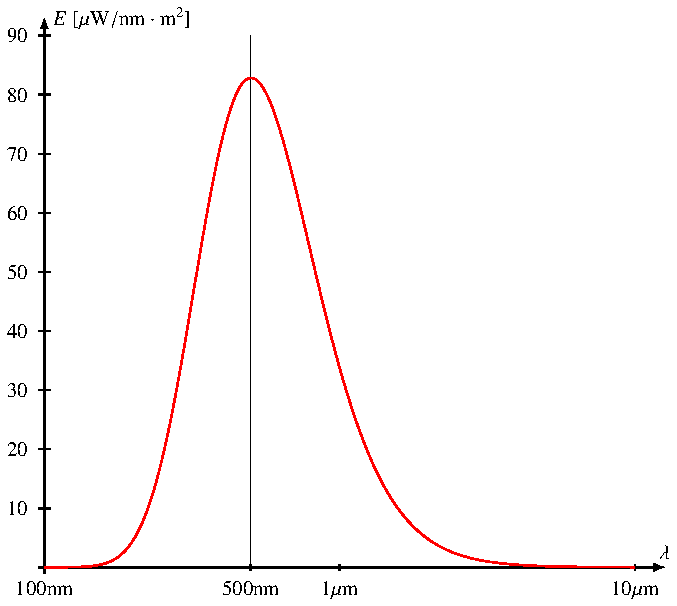
\includegraphics{chapters/1/planck.pdf}
\caption{Plancksches Strahlungsgesetz für die Sonne
\label{skript:planck-kurve}}
\end{figure}
\index{Plancksches Strahlungsgesetz}
\index{Strahlungsgesetz,Plancksches}
Die Strahlungsdichte in Abhängigkeit von der Wellenlänge ist in
Abbildung~\ref{skript:planck-kurve} dargestellt.
Die gesamte Strahlungsleistung ist das Integral
\[
P
=
\int_{0}^\infty E(\lambda,T)\,d\lambda
=
\int_{0}^\infty 
\frac{2\pi hc^2}{\lambda^5}\frac{d\lambda}{e^{\frac{hc}{\lambda kT}}-1}.
\]
Man beachte aber, dass in den graphischen Darstellungen des
Strahlungsspektrums eine logarithmische $\lambda$-Skala
verwendet wird.
Bei grossen Wellenlängen (``rechts'') wird die Kurve also in Wahrheit
viel stärker ausgedehnt.
Will man die Flächeninhalte unter den Kurven vergleichen, muss man
$E(\lambda,T)$ mit dem Faktor $\lambda$ skalieren.

\subsubsection{Einstrahlungswinkel}
Warum ist es in den Tropen wärmer als in gemässigten Breiten oder
an den Polen, wenn
die Sonne doch überall mit der gleichen Intensität einstrahlt.

Der Unterschied stammt natürlich vom Einstrahlungswinkel.
Der Ausdruck \eqref{skript:solarkonstante} für $P_{\earth}$ 
beschreibt die Strahlungsleistung pro Flächeneinheit, doch diese
Flächeneinheit wird senkrecht auf die Ausbreitungsrichtung der
Strahlung gemessen.
In gemässigten Breiten und an den Polen fällt die Strahlung 
in viel kleinerem Winkel auf die Erdoberfläche.
Die einfallende Energie verteilt sich daher auf eine grössere
Fläche.
Ist $\alpha$ der Winkel zwischen der Vertikalen und der Strahlungsrichtung,
dann ist die auf einer Erdoberfläche einfallende Strahlungsdichte nur
noch $P_{\earth}\cdot\cos\alpha$
(siehe auch Abbildung~\ref{skript:einfallswinkel}).

\begin{figure}
\centering
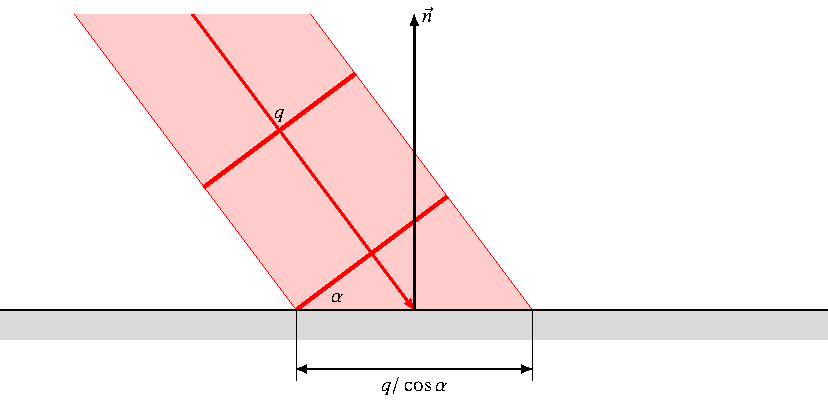
\includegraphics{chapters/1/einfall.pdf}
\caption{Einfluss des Einstrahlungswinkels auf die pro Flächeneinheit
der Erdoberfläche einfallende Strahlungsleistung.
Ein Strahlenbündel mit Querschnitt $q$, welches im Winkel
$\alpha$ zur Vertikalen einfällt, bedeckt die Fläche $q/\cos\alpha$
auf der Erdoberfläche.
\label{skript:einfallswinkel}}
\end{figure}

\subsubsection{Albedo\label{skript:subsubsection:albedo}}
\begin{table}
\centering
\begin{tabular}{|l|l|}
\hline
Material&Albedo\\
\hline
Frischer Schnee&0.8 -- 0.9\\
Wolken         &0.6 -- 0.9\\
Wüste          &0.3\\
Rasen          &0.18--0.23\\
Wald           &0.05--0.18\\
Wasserfläche   &0.05--0.22 (winkelabhängig)\\
Erde           &0.306 \\
Mond           &0.11 \\
\hline
\end{tabular}
\caption{Albedo verschiedener Oberflächen und Himmelskörper
(aus \cite{skript:albedo})
\label{skript:albedotabelle}}
\end{table}
Die Erde ist noch weniger perfekter schwarzer Strahler als die Sonne.
Die Ausstrahlung enthält zwar die Strahlung eines schwarzen Körpers mit
der Mitteltemperatur als Temperatur $T$,
sie ist aber überlagert von der Strahlung, die vom Erdboden oder von
Wolken reflektiert wird.
Die {\em Albedo} ist der Anteil der reflektierten Strahlung, also ein
Wert zwischen $0$ und $1$.
\index{Albedo}
Tabelle~\ref{skript:albedotabelle} stellt einige interessante
Albedo-Werte von verschiedenen Oberflächen zusammen.

Die Albedo hat eine direkte Auswirkung auf das Klima, umgekehrt
hängt die Albedo aber auch vom Klima ab.
Nimmt die Bewölkung zu, steigt die Albedo, es erreicht weniger 
Strahlung die Erdoberfläche.
Schneefall erhöht ebenfalls die Albedo.
Umgekehrt reduziert das Abschmelzen der Polkappen oder der
Schneedecke in Permafrostgebieten die Albedo, so dass mehr Strahlung
von der Erdoberfläche absorbiert wird.

\subsubsection{Strahlungsbilanz}
\begin{figure}
\centering
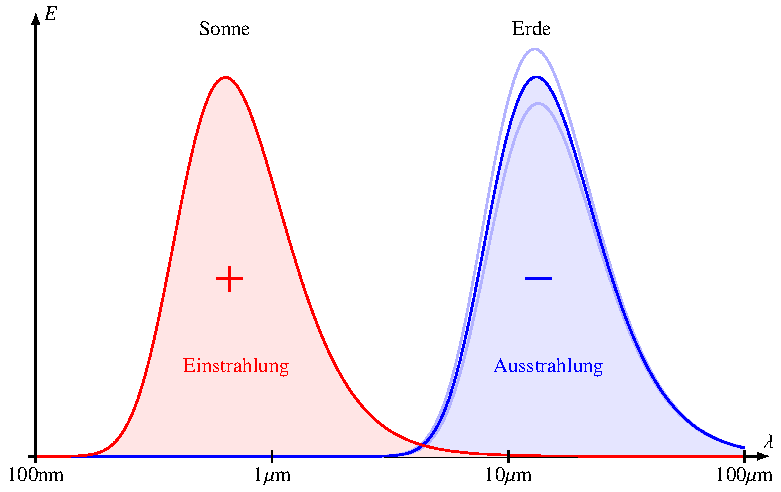
\includegraphics{chapters/1/vergleich.pdf}
\caption{Strahlung der Sonne (rot) und der Erde (blau).
Das Maximum der Strahlung der Sonne ist im sichtbaren Bereich,
das Maximum der Wärmestrahlung der Erde im Infraroten.
\label{skript:strahlung-sonne-erde}}
\end{figure}%
In Abbildung~\ref{skript:strahlung-sonne-erde} sind die Planckschen
Strahlungskurve für die Sonne und Erde derart skaliert dargestellt,
dass die Flächen unter den Strahlungs direkt als Mass für die gesamte
Strahlungsleistung dienen können.
Die rote Kurve zeigt die spektrale Strahlungsleistung, die von der
Sonne auf den Querschnitt $\pi R_{\earth}^2$ der Erde eingestrahlt wird,
also
\[
E(\lambda,T_{\astrosun}) \cdot 2\pi R_{\earth}^2
\cdot
\biggl(\frac{R_{\astrosun}}{a_{\earth}}\biggr)^2
\]
mit $T_{\astrosun}=5778\text{K}$.
Die dunkelblaue Kurve zeigt das Ausstrahlungsspektrum der ganzen Erde mit
einer Temperatur von $T=279\text{K}$, also
\[
E(\lambda,T_{\earth})\cdot 4\pi R_{\earth}^2.
\]
Die Fläche unter der Kurve ist ein Mass für die gesamte Energie.
Offenbar halten sich Einstrahlung und Ausstrahlung die Waage.

Die Einstrahlung kann sich zum Beispiel dann verändern, wenn 
mehr Strahlung reflektiert wird.
Die Ausstrahlung dagegen verringert sich, wenn die Atmosphäre für infrarote
Strahlung undurchsichtiger wird, wie dies zum Beispiel durch
erhöhte $\text{H}_2\text{O}$- oder $\text{CO}_2$-Konzentration geschehen kann.
Damit sich wieder ein Gleichgewicht einstellt, muss sich die Temperatur der
Erde erhöhen, damit die Ausstrahlung ebenfalls höher wird
(obere hellblaue Kurve in Abbildung~\ref{skript:strahlung-sonne-erde}).
Sinkt der Gehalt an Treibhausgasen, wird die Atmosphäre transparenter
für Wärmestrahlung,
ein Gleichgewicht ist möglich bei tieferer Temperatur (untere
hellblaue Kurve).
Diese Abhängigkeit der Temperatur von der Transparenz der
Atmosphäre für Wärmestrahlung ist bekannt als der {\em Treibhauseffekt}.
\index{Treibhauseffekt}

\subsubsection{Tatsächliches Strahlungspektrum}
\begin{figure}
\centering
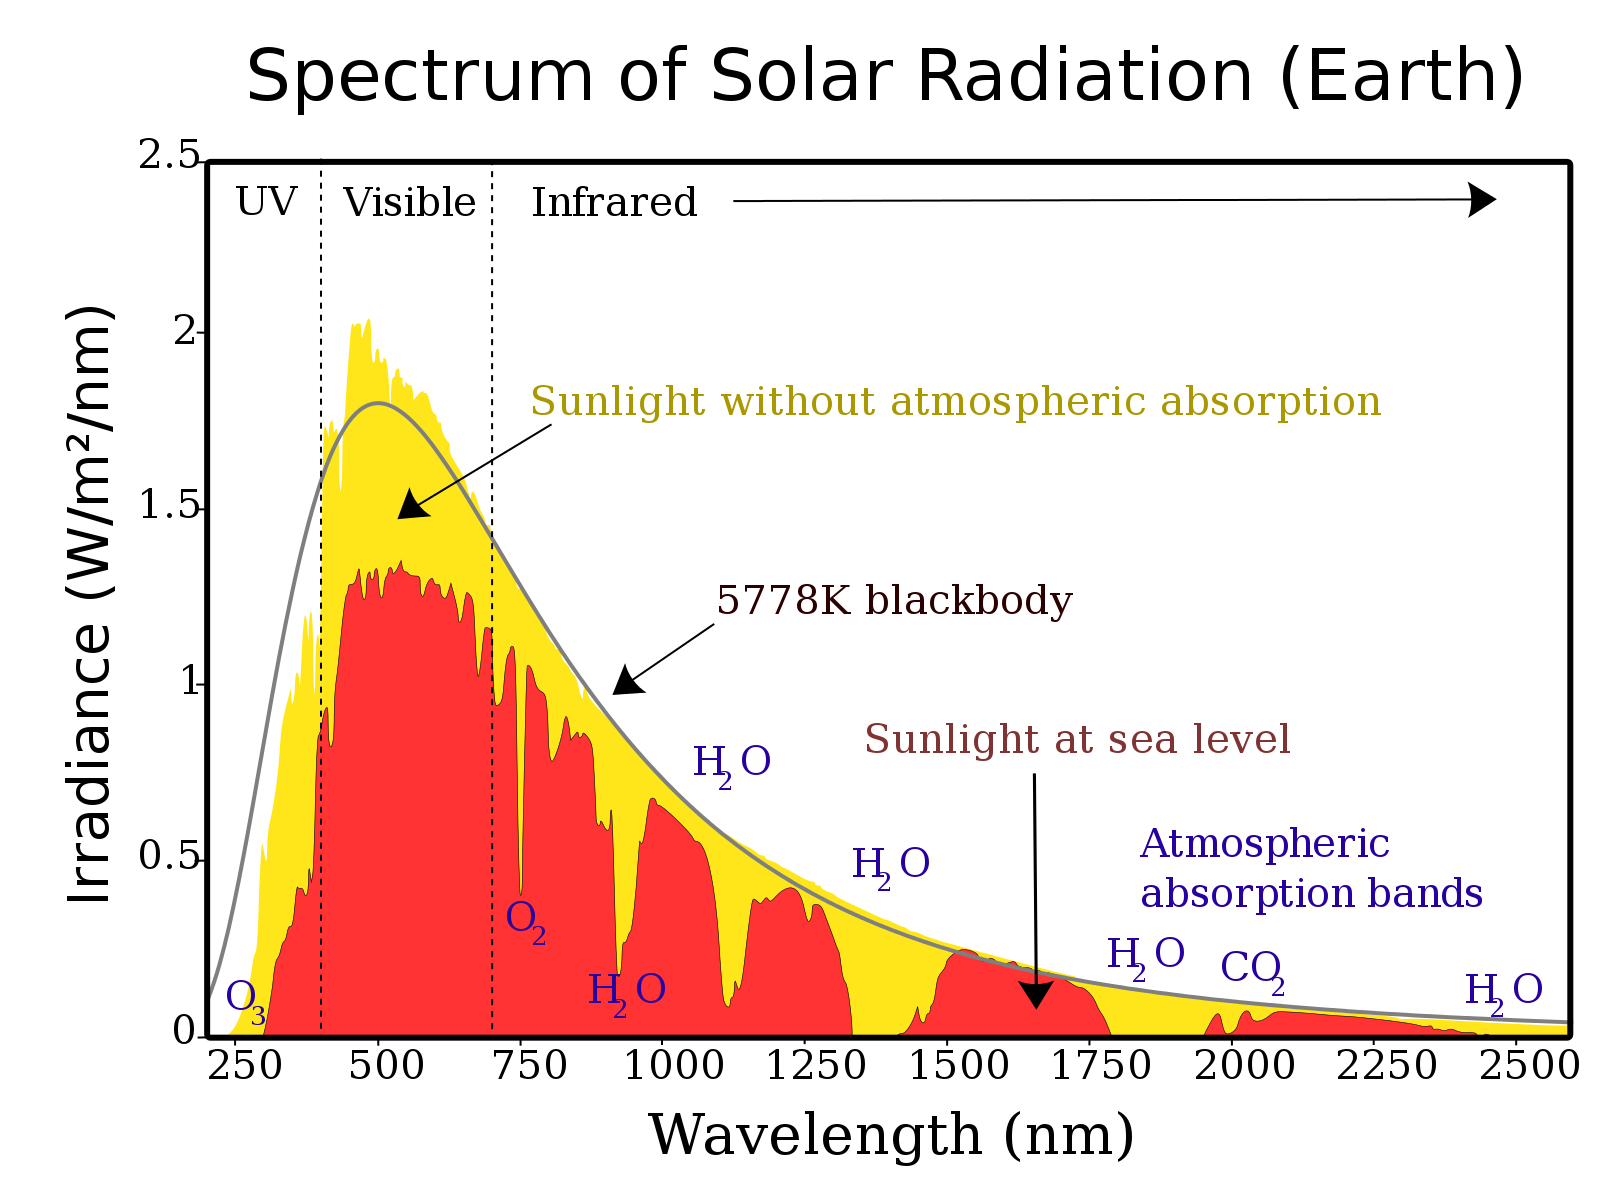
\includegraphics[width=0.7\hsize]{chapters/1/Solar_spectrum_en.png}
\caption{Tatsächliches Spektrum der Sonnenstrahlung mit (rot) und
ohne (gelb) atmosphärische Absorbtion im Vergleich mit dem Spektrum
der Schwarzkörperstrahlung \cite{skript:sunlight}.
\label{skript:strahlungsspektrum}}
\end{figure}
In Abbildung~\ref{skript:strahlungsspektrum} ist das tatsächlich gemessene
Strahlungsspektrum der Sonne dargestellt.
Es fällt auf, dass Wasserdampf und $\text{CO}_2$  für bedeutende
Absorbtionsbänder im Infraroten verantwortlich ist,
während im sichtbaren bereich
die Absorbtion sehr gleichmässig ist.

\subsection{Erdrotation und atmosphärische Zirkulation\label{skript:section:zirkulation}}
Die Einstrahlung ist wegen des grösseren Einstrahlungswinkels
am grössten am Äquator, während an den Polen die Ausstrahlung überwiegt.
Dies führt dazu, dass die Temperatur an den Polen tiefer ist.
Da sich die Erde im Gleichgewicht befindet, bedeutet dieser
Temperaturunterschied aber auch, dass Prozesse in
der Atmosphäre Energie aus niedrigen Breiten zu den Polen
transportieren müssen.
Die Temperaturunterschiede sind jedoch zu klein dafür, dass Wärmeleitung
den Transport bewerkstelligen könnte.
Die Energie muss daher durch Advektion (S.~\pageref{skript:advektion})
unterstützt von latenter Wärme transportiert werden.
Um den Energiehaushalt des globalen Klimasystems zu verstehen, muss
\index{globale Zirkulation}%
\index{Zirkulation, globale}%
man daher die globalen Strömungen in der Atmosphäre aber auch in
den Ozeanen verstehen.

In Kapitel~\ref{chapter:fluiddynamik} werden die Grundgleichungen
der Fluiddynamik besprochen.
In diesem Abschnitt beschränken wir uns auf eine qualitative
Diskussion der globalen Zirkulation.
Die globale Zirkulation unterscheidet sich von Strömungen, die 
in technischen Anwendungen üblicherweise studiert werden dadurch,
dass sie zwar im allgemeinen langsamer ist, dafür aber ein viel grössers
Volumen und grössere Distanzen umfasst.
Die Windsysteme, die für die Wetterphänomene verantwortlich sind,
haben typische Abmessungen von hunderten oder sogar tausenden von
Kilometern.

\subsubsection{Druckunterschiede und Euler-Wind}
Windströmungen in der Atmosphäre werden von Druckunterschieden
hervorgerufen.
Die Sonnenstrahlung erwärmt die Erdoberfläche und mittelbar die
Atmosphäre.
Die warme Luft hat geringere Dichte und steigt daher auf.
Damit nimmt die Kraft ab, die die Luft auf darunterliegenden
Schichten ausüben kann, es entsteht ein Unterdruck.
Man nennt eine Luftströmung, die nur durch Druck\-unterschiede
unter Vernachlässigung von Corioliskraft, Zentrifugalkraft und
Reibung entsteht, den {\em Euler-Wind}.
\index{Euler-Wind}
Lokale Wind-Systeme wie Land-See-Wind oder Berg-Tal-Wind sind von
dieser Art.

\subsubsection{Coriolis-Effekt}
\index{Coriolis-Kraft}%
\index{Coriolis-Effekt}%
Die Erde dreht sich in 23 Stunden 56 Minuten und 4.091 Sekunden
einmal um sich selbst (siderische Rotationsperiode).
\index{siderische Rotationsperiode}%
Die Drehung kann mit dem Winkelgeschwindigkeitsvektor
$\vec{\Omega}$
beschrieben werden, der die Richtung der Erdachse vom Süd- zum Nordpol
hat und als Länge die Winkelgeschwindigkeit
\[
\omega
=
|\vec{\Omega}|
=
\frac{2\pi}{86164.091\,\text{s}}.
\]
Ein Körper, der sich relativ zu einem mit der Erde verbundenen
Koordinatensystem mit der Geschwindigkeit $\vec{v}$ bewegt,
erlebt eine durch die Drehung verursachte Coriolis-Beschleunigung
\[
\vec{a} = -2\vec{\Omega}\times\vec{v}.
\]
Ein Flugzeug, welches mit 880\,km/h über den Nordpol fliegt,
erfährt dort die Beschleunigung 
\[
|\vec{a}|
=
\biggl|
-2
\cdot
\frac{2\pi}{86164.091\,\text{s}}
\cdot
244.44\frac{\text{m}}{\text{s}}
\biggr|
=
0.01782\frac{\text{m}}{\text{s}^2}.
\]
Diese Beschleunigung ist viel zu klein, dass sie einen wesentlichen
Einfluss auf die Bahn eines Flugzeugs haben könnte.
Der Luftwiderstand und die von den Steuerflächen des Flugzeugs erzeugten
Kräfte und die daraus resultierenden Beschleunigungen sind
um Grössenordnungen grösser.
In der freien Atmosphäre wirkt auf die Luft jedoch nur die Druckkraft,
so dass die Coriolis-Beschleunigung einen dominanten Einfluss bekommt.

\begin{figure}
\centering
\begin{tikzpicture}[scale=1, >= latex]
\node at (0,0) {
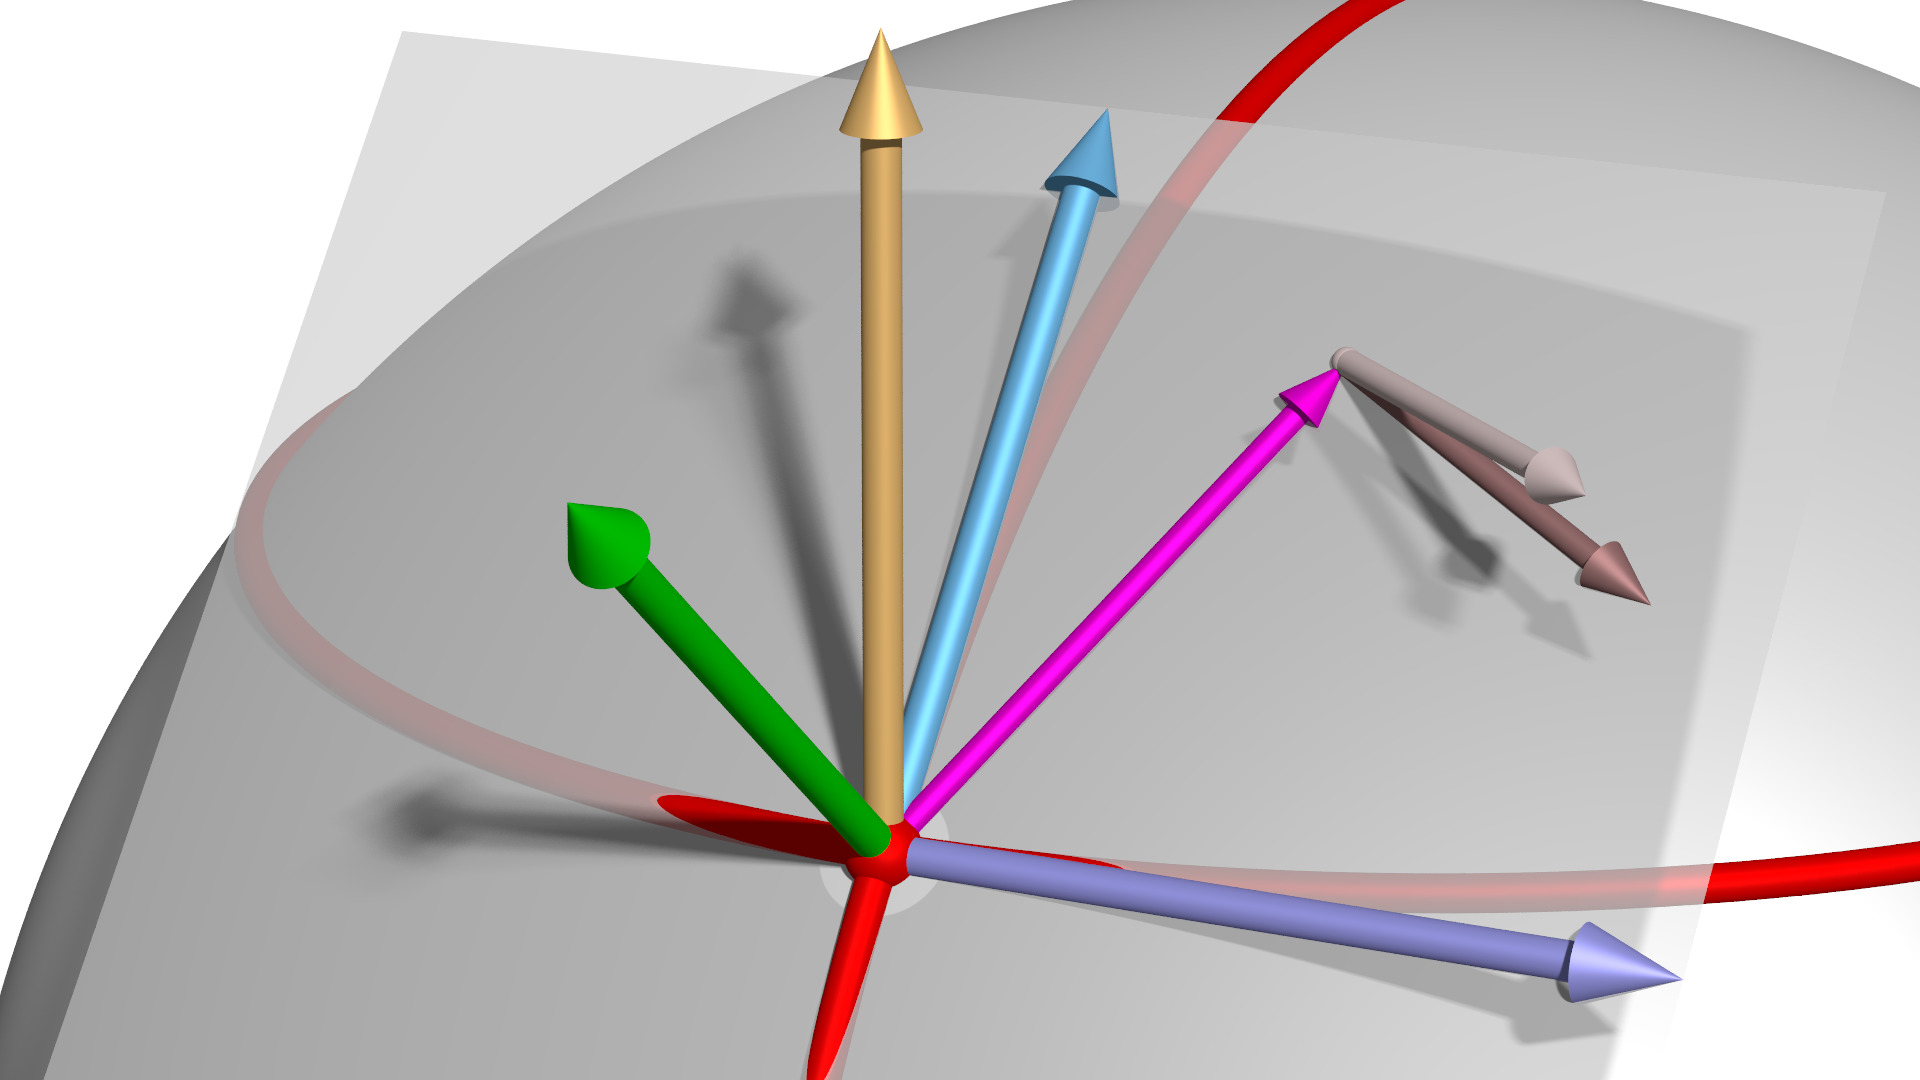
\includegraphics[width=\hsize]{chapters/1/betaplane.jpg}
};
%\node at (0,0) {$\bullet$};
%\node at (1,0) {$\bullet$};
%\node at (-1,0) {$\bullet$};
%\node at (0,1) {$\bullet$};
%\node at (0,-1) {$\bullet$};
\node at (-0.3,-2.7) {$B$};
\node at (5.1,-2.7) {$U$};
\node at (1.4,2.9) {$V$};
\node at (-0.6,4.1) {$\vec{\Omega}$};
\node at (-3,0.6) {$\vec{n}$};
\node at (2.3,1.4) {$\vec{v}$};
\node at (4.5,1) {$-2\vec{\Omega}\times\vec{v}$};
\node at (6,-0.5) {$(-2\vec{\Omega}\times\vec{v})_{\|}$};
\end{tikzpicture}
\caption{$\beta$-Ebene: Koordinatensystem in der Tangentialgebene an die Kugel
im Punkt $B$ mit Achsen $U$ parallel zu Breitenkreisen und $V$ parallel
zu Längenkreisen.
Die Normale der Tangentialebene ist $\vec{n}$.
Ebenfalls eingezeichnet die Coriolis-Beschleunigung
$-2\vec{\Omega}\times\vec{v}$ zur Geschwindigkeit $\vec{v}$ und
die Komponente $(-2\vec{\Omega}\times\vec{v})_{\|}$ parallel
zur Tangentialebene.
\label{skript:betaplane}}
\end{figure}
Die grossräumige Strömung in der Erdoberfläche verläuft im Wesentlichen 
parallel zur Erdoberfläche.
Daher interessiert für die Beschreibung der Wirkung des Coriolis-Effekts
vor allem die Komponente der Beschleunigung parallel zur Erdoberfläche.
In einem Punkt $B$ der Erdoberfläche verwenden wir daher ein
Koordinatensystem in der Tangentialebene so, dass die $x$-Achse tangential
zum Breitenkreis in $B$ ist und die $y$-Achse tangential zum Längenkreis
(Abbildung~\ref{skript:betaplane}).
Die tangentiale Geschwindigkeit wird in diesem Koordinatensystem durch die
Komponenten $u$ in $U$-Richtung und $v$ in $V$-Richtung beschrieben.
Dieses Koordinatensystem in der Tangentialebene im Punkt $B$ heisst auch
die {\em $\beta$-Ebene}.
\label{skript:betaplane:definition}
\index{$\beta$-Ebene}

Wir berechnen die Coriolis-Beschleunigung in diesem Koordinatensystem.
Für einen Geschwindigkeitsvektor $\vec{v}$ parallel zu $V$ hat das
Vektorprodukt $\vec{\Omega}\times \vec{v}$ bereits die Richtung $U$,
er muss also nicht mehr in die Tangentialebene projiziert werden.
Der Winkel zwischen $\vec{\Omega}$ und $V$ ist die geographischen Breite
$\alpha$.
Die Coriolis-Beschleunigung ist daher $2\omega \sin(\alpha)u\cdot V$.

Für einen Geschwindigkeitsvektor $\vec{v}$ parallel zu $U$ steht
das Vektorprodukt $-2\vec{\Omega}\times\vec{v}$ senkrecht auf 
der Erdachse.
Da $U$ und $\vec{\Omega}$ senkrecht stehen, ist der Betrag der 
Coriolis-Beschleunigung
\[
|\text{$-2\vec{\Omega}\times\vec{v}$}|
=
2\omega u.
\]
\begin{figure}
\centering
\begin{tikzpicture}[scale=1, >= latex, thick]
\draw[->] (0,-4.5)--(0,4.5) coordinate[label={$z$}];
\draw (0,0) circle[radius=4];
\def\a{70}
\coordinate (B) at ({-4*sin(\a)},{4*cos(\a)});
\node at (B) [above left] {$B$};
\coordinate (C) at ({-4*sin(\a)},{4*cos(\a)+3});
\coordinate (D) at ({-4*sin(\a) - 3},{4*cos(\a)});
\coordinate (E) at ({-4*sin(\a) + 10 * cos(\a)},{4*cos(\a) + 10 * sin(\a)});
\coordinate (F) at ({-4*sin(\a) - 10 * cos(\a)},{4*cos(\a) - 10 * sin(\a)});
\def\l{-3*cos(\a)}
\coordinate (G) at ({-4*sin(\a) + \l*cos(\a)},{4*cos(\a) + \l*sin(\a)});
\draw[line width=0.1] (D)--(G);
\draw (0,0)--(B);
\draw (-4.5,0)--(4.5,0);
\node at (-0.8,0) [above left] {$\alpha$};
\draw[->,line width=1.5pt] (B)--(C) coordinate[label={above left:$\vec{\Omega}$}];
\draw[->] (B)--(D) coordinate[label={above:$-2\vec{\Omega}\times\vec{v}$}];
\begin{scope}
\clip (-7,-4.5) rectangle (4.5,5);
\draw (E)--(F);
\end{scope}
\draw[color=red,line width=1.7pt,->] (B)--(G);
\fill[color=red] (B) circle[radius=0.09];
\end{tikzpicture}
\caption{Berechnung der Coriolis-Beschleunigung für einen
Geschwindigkeitsvektor in $U$-Richtung.
\label{skript:U-coriolis}}
\end{figure}%
Aus Abbildung~\ref{skript:U-coriolis} kann man ablesen,
dass die Komponente der Coriolis-Beschleunigung parallel
zur Tangentialebene $2\omega u\sin(\alpha)$ ist.

Setzen wir die beiden Resultate zusammen finden wir, dass die
Coriolis-Beschleunigung im $U$-$V$-Koordinatensystem
\begin{equation}
\underbrace{
2\omega
\sin\alpha}_{\displaystyle=f}
\begin{pmatrix}
v\\
-u
\end{pmatrix}
\label{skript:physik:coriolis}
\end{equation}
ist.
Die Coriolis-Beschleunigung ist proportional zu $f=2\omega\sin\alpha$, auch
bekannt als der {\em Coriolis-Parameter}.
\index{Coriolis-Parameter}%

\subsubsection{Globale Zirkulation}
Die bisher besprochenen Prinzipien ermöglichen uns, die
global Zirkulation qualitativ zu beschreiben.
Veränderungen der globalen Zirkulation sind langsam,
es ist daher gerechtfertigt, die täglichen Schwankungen der
Einstrahlung infolge der Erdrotation durch eine mittlere
Einstrahlung zu ersetzen.
Die Bedingungen für die globale Zirkulation sind daher rotationssymmetrisch
um die Erdachse.
Wir suchen daher nach einem globalen Strömungsmuster, welches ebenfalls
rotationssymmetrisch ist.

\begin{figure}
\centering
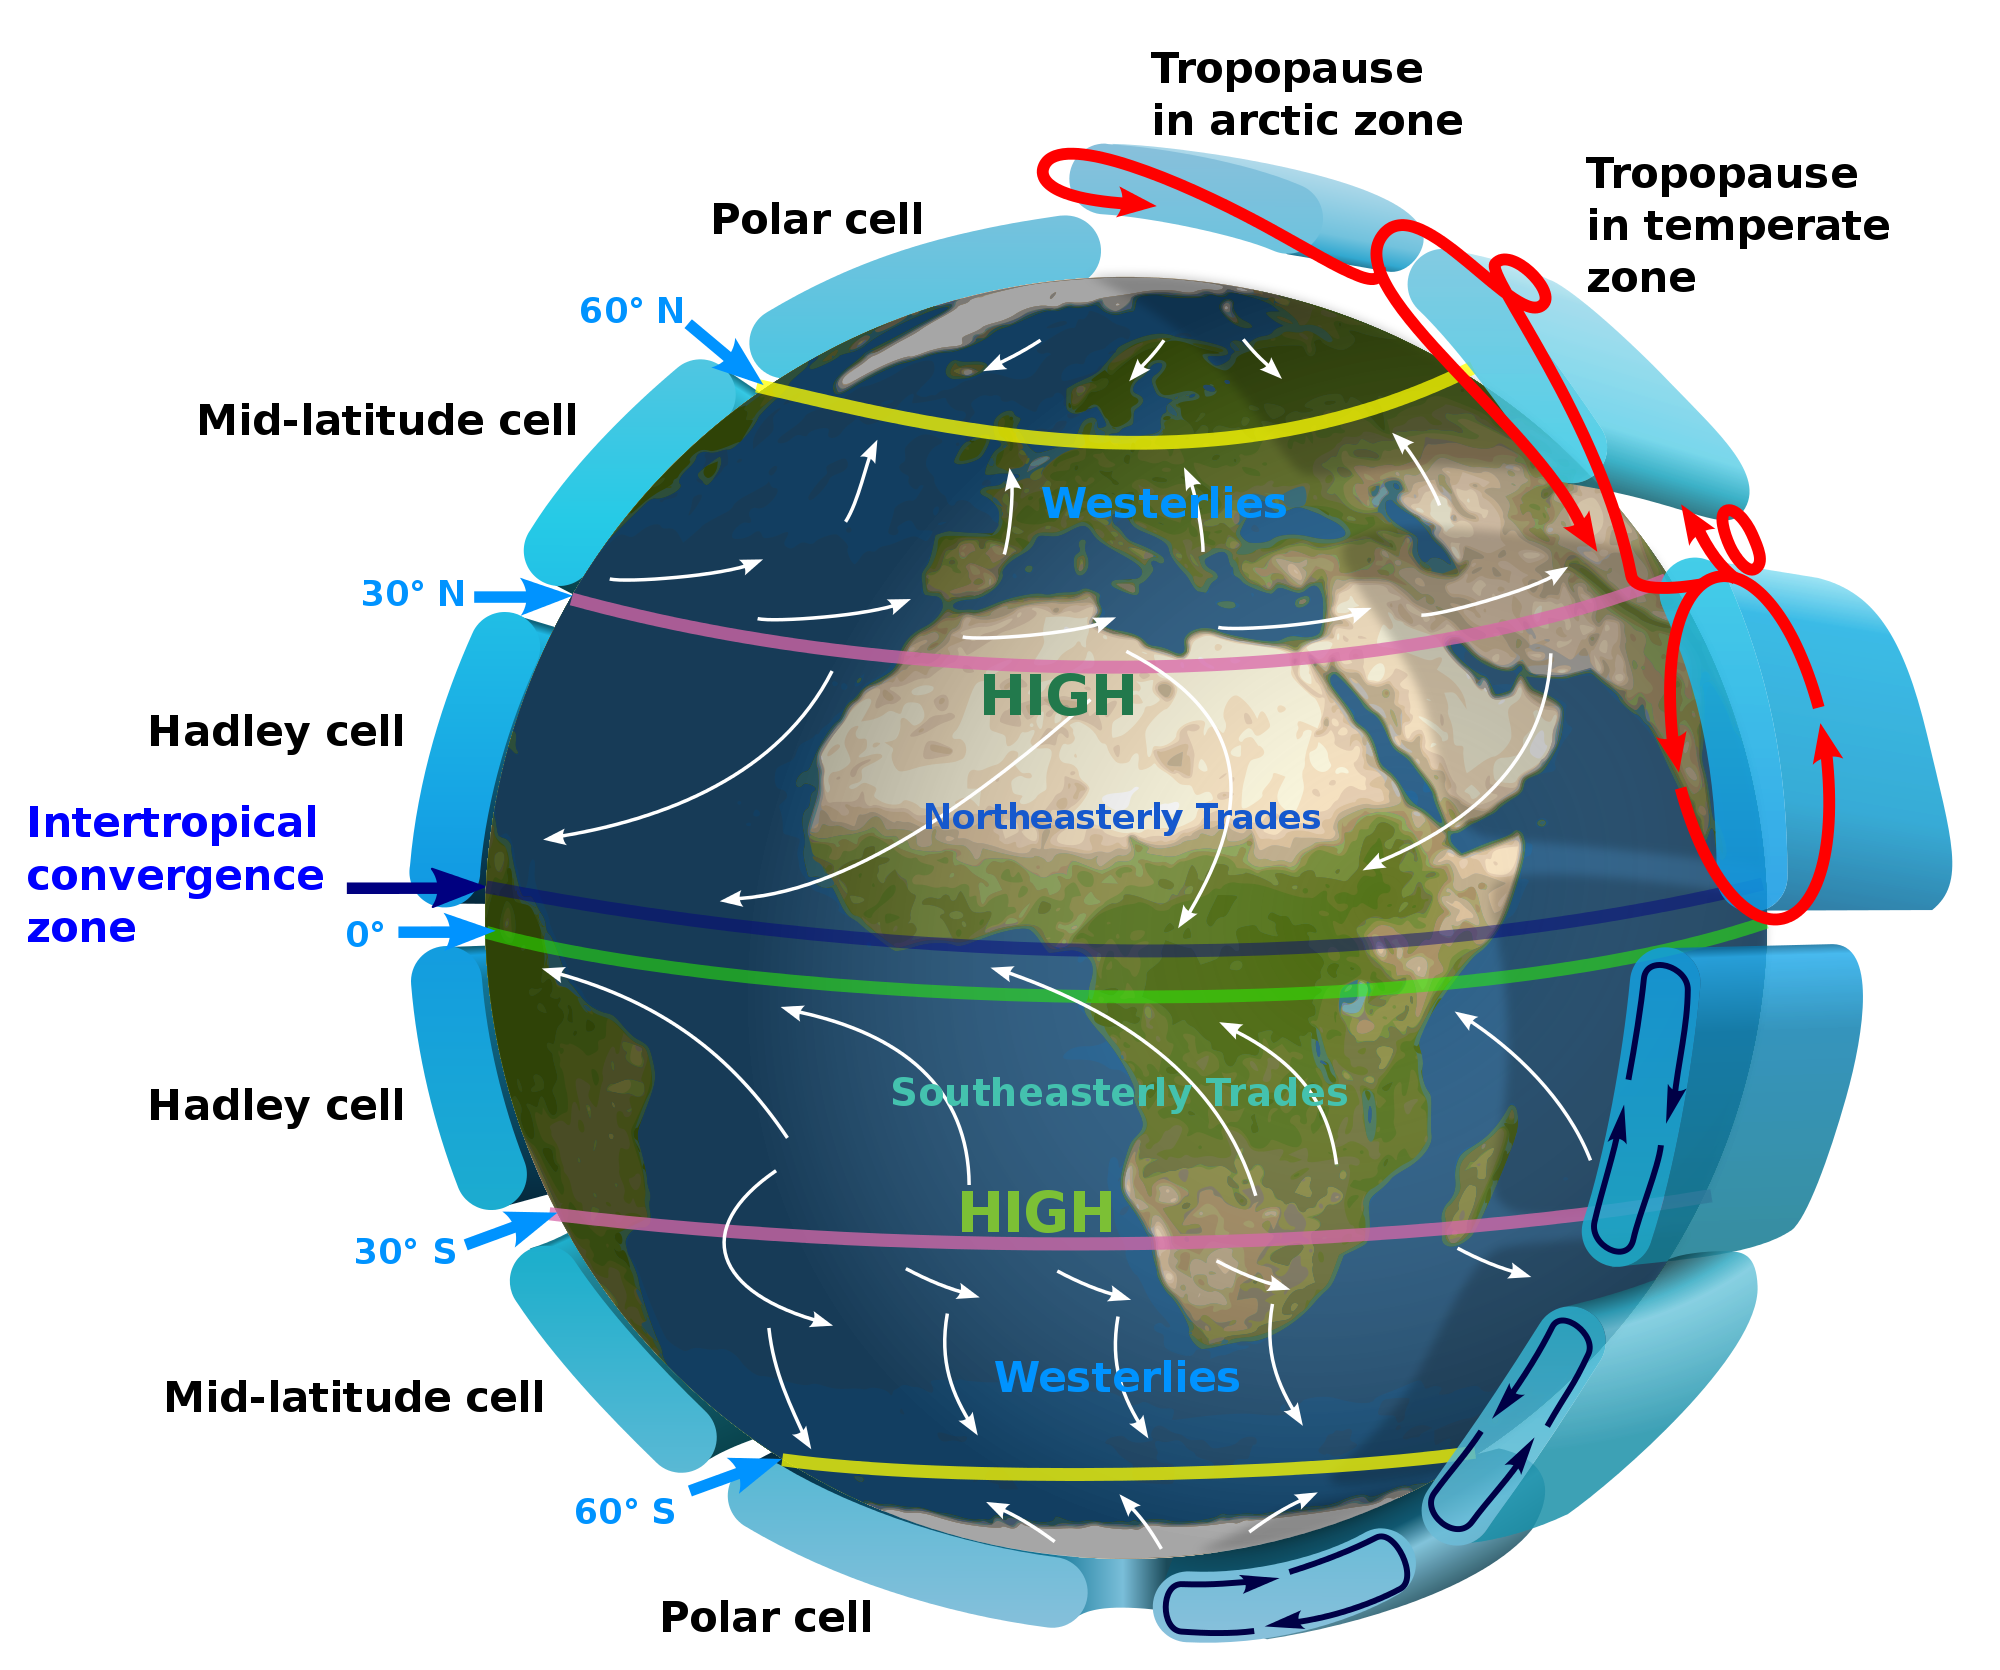
\includegraphics[width=\hsize]{chapters/1/Earth_Global_Circulation_-_en.png}
\caption{Globale Zirkulation der Erde
\label{skript:globalezirkulation}}
\end{figure}

Die grösste Einstrahlung erfolgt am Äquator, erwärmt die Luft und
lässt sie aufsteigen.
Der entstehenden Unterdruck in Äquatornähe erzeugt eine 
Ausgleichsströmung in Bodennähe.
Die aufsteigende Luft kann nicht beliebig hoch aufsteigen und weicht
daher in grosser Höhe in Richtung der Pole aus.
Die Höhenströmung nach Norden wird von der Coriolis-Beschleunigung nach
rechts abgelenkt, sie kann also nicht beliebig weit nach Norden
strömen, bevor sie wieder absinkt.
Es entsteht je eine geschlossene Konvektionszelle wie in
Abbildung~\ref{skript:globalezirkulation}, die sogenannte
Hadley-Zelle \cite{skript:hadley}.

Im Anschluss an die Hadley-Zellen entstehen auf Grund des gleichen
Mechanismus weitere Zellen.
Die Breite der Zellen hängt offenbar von der Stärke des Coriolis-Effektes ab.
Auf einem Planeten mit grösserer Rotationsgeschwindigkeit erwartet man
vergleichsweise schmalere Zellen.
\begin{figure}
\centering
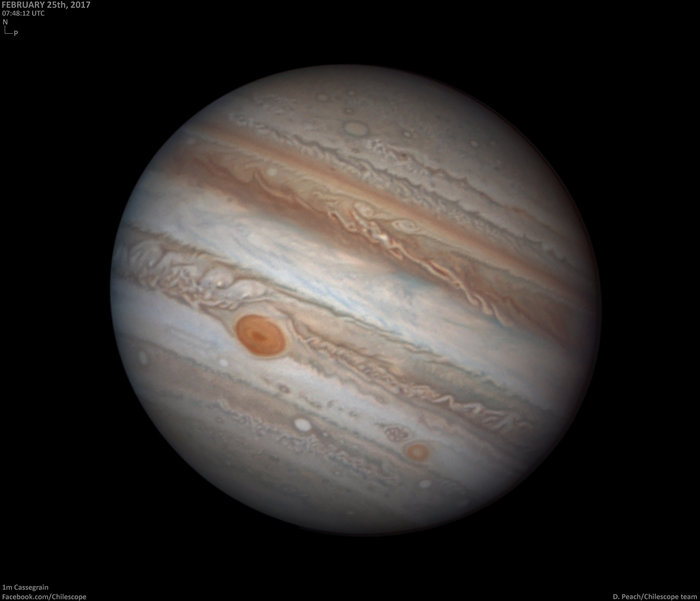
\includegraphics[width=\hsize]{chapters/1/Jupiter_on_25_February_2017_node_full_image_2.jpg}
\caption{Jupiter mit Wolkenbändern, Aufnahme von Damian Peach
\cite{skript:jupiter}
\label{skript:jupiterzirkulation}}
\end{figure}
Dies ist genau was man am Beispiel der globalen Strömung auf dem
Jupiter in Abbildung~\ref{skript:jupiterzirkulation} beobachten kann.

\subsubsection{Äquatorialzone}
Nahe dem Äquator ist die geographische Breite $\alpha$ klein und
damit auch der Coriolis-Parameter $f$.
Die Strömung in Äquatornähe ist daher praktisch unbeeinflusst 
vom Coriolis-Effekt.
Entlang des Äquators kann die Luft oder das Meer also
unbeeinflusst durch die Coriolis-Beschleunigung strömen.

Mit Hilfe der $\beta$-Ebene können wir jetzt aber auch modellhaft 
die Bewegung eines Massepunktes in Äquatornähe berechnen.
Wenn die Coriolis-Beschleunigung der einzige Einfluss ist, dann
\begin{equation}
\frac{d}{dt}
\begin{pmatrix}u\\v\end{pmatrix}
=
f\begin{pmatrix}v\\-u\end{pmatrix}.
\end{equation}
Der Coriolis-Parameter $f=2\omega\sin\alpha$ ist proportional
zur geographischen Breite.
Für nicht zu grosse geographische Breiten können wir $\sin\alpha$ durch
die $y$-Koordinate erstzen.
Wir müssen also die Differentialgleichung
\begin{equation}
\frac{d}{dt}
\begin{pmatrix}x\\y\\u\\v\end{pmatrix}
=
\begin{pmatrix}
u\\v\\fyv\\-fyu
\end{pmatrix}.
\label{skript:coriolis-dgl}
\end{equation}
lösen.
Die Gestalt der Lösungskurven hängt von der Anfangsgeschwindigkeit und
vom Parameter $f$ ab.
Für $f=0$ fällt die Coriolis-Beschleunigung ganz weg, in diesem
Fall sind die Lösungskurven Geraden.

\begin{figure}
\centering
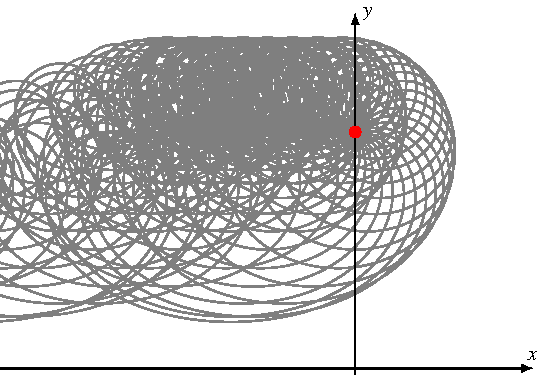
\includegraphics{chapters/1/stream.pdf}
\caption{
Lösungen der Differentialgleichung ausgehend vom Punkt $(0,4)$
mit Anfangsgeschwindigkeit $|\vec{v}|=1$ und $f=0.26$.
Die Bahnkurven sind immer nach rechts gekrümmt und bleiben in der
oberen Halbebene.
\label{skript:stream-graph}}
\end{figure}

\begin{figure}
\centering
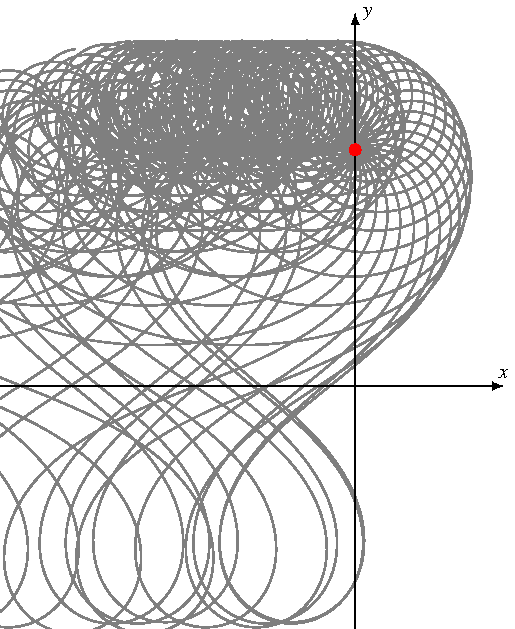
\includegraphics{chapters/1/cross.pdf}
\caption{
Lösungen der Differentialgleichung ausgehend vom Punkt $(0,4)$
mit Anfangsgeschwindigkeit $|\vec{v}|=1$ und $f=0.22$.
Einzelne Bahnkurven kreuzen die $x$-Achse und krümmen sich in der unteren
Halbeben dann links.
\label{skript:cross-graph}}
\end{figure}

Um einen Überblick über die möglichen Lösungskurven zu erhalten, berechnen
wir numerisch die vom Punkt $(0,4)$ ausgehenden Lösungskurven 
der Differentialgleichung~\ref{skript:coriolis-dgl}.
Je grösser $f$ ist, desto stärker gekrümmt sind die Lösungskurven.
Solange die Kurven in der oberen Halbebene $y>0$ liegen sind die Kurven
nach rechts gekrümmt.
Für genügend grosses $f$ bleiben alle Kurven in der oberen
Halbebene wie in Abbildung~\ref{skript:stream-graph}, unabhängig
von der Richtung der Anfangsgeschwindigkeit.
Für kleinere Werte von $f$ wie in Abbildung~\ref{skript:cross-graph}
gelangen einzelne Bahnkurven in die untere Halbebene wo die Krümmung
der Kurve von rechts auf links kehrt.

Man beachte, dass diese Bahnkurven nicht Stromlinien einer Strömung sind,
da sich diese nicht kreuzen können.
Dieses einfache Modell ist also nicht geeignet, die tatsächliche Bewegung
der Luftmassen darzustellen, dazu müssen wir die Gleichungen
der Fluiddynamik in Kapitel~\ref{chapter:fluiddynamik}.

\subsubsection{Meeresströmungen}
Meeresströmungen leisten einen bedeutenden Beitrag zum Klima, weil sie
dank der hohen Wärmekapazität von Wasser auch bei kleiner
Strömungsgeschwindigkeit und sehr viel kleinerem bewegtem Volumen als
bei den atmosphärischen Strömungen eine grosse Energiemenge transportieren
können.

\subsection{Periodische Einflüsse}
Das Klimasystem ist einer Reihe von sich periodisch verändernden 
Einflüssen ausgesetzt.
Viele dieser Einflüsse erscheinen auf den ersten Blick geringfügig
und damit vernachlässigbar.
Doch wenn ein solcher periodischer Einfluss mit einer Frequenz auftritt,
der einer Eigenfrequenz des Klimasystems entspricht, dann kann sich 
in Folge eines Resonanzeffektes über längere Zeit ein bedeutender 
Einfluss auf das Klima manifestieren.
Es ist daher wichtig, auch kleine Einflüsse zu kennen und insbesondere
alle Aspekte des Klimasystems zu modellieren, die eine Eigenfrequenz
in der Nähe ihrer Anregungsfrequenzen haben.

\subsubsection{Sonnenfleckenzyklus}
\index{Sonnenflecken}%
\index{Sonnenfleckenzyklus}%
Die Strahlung der Sonne ist nicht konstant.
Wie bei jedem Stern dieser Klasse nehmen Durchmesser und Temperatur der
Sonne über die Jahrmillionen in dem Mass zu, dass neben der Fusion
von Wasserstoff zu Helium auch noch Fusionsprozesse schwerer Elemente
eine Rolle zu spielen beginnen.
Dieser sehr langfristige Einfluss ist jedoch nur wesentlich für
den Vergleich von Klimamodellen mit Daten über das Klima auf der sehr
jungen Erde.

Für kurzfristige Prognosen von Bedeutung sind dagegen die Schwankungen
der Sonnenaktivität.
\index{Sonnenaktivität}%
Die Zahl der Sonnenflecken ist ein leicht zu messender Indikator
dafür, für den Aufzeichnung seit dem 17.~Jahrhundert existieren.
Die Sonnenfleckenzahl schwankt mit einer Periode von etwa elf Jahren.
Die daraus resultierende Änderung der Einstrahlung ist jedoch nur 0.07\%,
so dass die Sonnenaktivität nicht für den Klimawandel verantwortlich
gemacht werden kann. 
Die schwankende Sonnenaktivität muss jedoch bei der Validierung
von Klimamodellen berücksichtigt werden.

\subsubsection{Bahnänderungen der Erde}
\index{Bahnänderungen}%
Nach Kepler bewegen sich die Planeten auf Ellipsen,
in deren einem Brennpunkt die Sonne steht.
Die keplerschen Gesetze der Planetenbahnen können aus dem Newtonschen 
Gravitationsgesetz hergeleitet werden
\cite[\S 6]{skript:joos}.
\index{Bahnelemente}%
\index{Keplersche Gesetze}%
Die Bahnelemente beschreiben die Ebene, in der sich der Planet bewegt,
die Richtung und der Zeitpunkt der grössten Annäherung an die Sonne und
die Exzentrizität der Ellipse.
\index{Exzentrizität}%
%
Es trifft exakt jedoch nur dann zu, wenn keine anderen Kräfte auf den
Planeten wirken als die Anziehungskraft der Sonne.
Newtons Gravitationsgesetz besagt nämlich, dass auch alle anderen
\index{Gravitationsgesetz}%
Planeten durch ihre Schwerkraft auf die Erde einwirken.
Dies äussert sich darin, dass sich die Bahnelemente mit der Zeit
ändern.
Diese langsame Veränderung der Bahnelemente war schon Newton bekannt,
er hat daraus geschlossen, dass das Sonnensystem mit der Zeit völlig
zerfallen würde.
Genauere Untersuchungen und numerische Rechnungen zeigen jedoch, dass
unser Sonnensystem über lange Zeit stabil ist.
Die Exzentrizität zum Beispiel der Erdbahn kann sich tatsächlich verändern,
aber über längere Zeit wird die Veränderung auch wieder rückgängig
gemacht.

Veränderungen der Erdbahn, insbesondere der Exzentrizität, oder der
Neigung der Erdachse zur Bahn äussern sich darin, dass die Einstrahlung
über das Jahr stärker oder weniger stark schwankt oder auch im Mittel
grösser oder kleiner wird.
\index{Neigung der Erdachse}%
Dadurch können sich die Temperaturunterschiede zwischen den Polgebieten und
äquatorialen Breiten verändern und damit die Intensität des Wettergeschehens
beeinflusst werden.
Ein langfristiges Klimamodell muss also auch diese Änderungen
modellieren.

Es stellt sich allerdings heraus, dass diese Veränderungen sehr viel
langfristiger sind als der die meisten Klimapolitiker interessierenden
Zeitraum von wenigen Jahrhunderten.
Die Berücksichtigung dieser Effekte dient daher vor allem dazu die
Klima-Modelle mit der Klimageschichte der Erde zu vergleichung und
damit zu validieren.
In Kapitel~\ref{chapter:fourier} wird gezeigt, wie periodische Einflüsse
modelliert und mit Hilfe der Fourier-Theorie analysiert werden können.
Und in Kapitel~\ref{chapter:neigung} wird gezeigt, wie die periodischen
Störungen der Erdbahnneigung zu dramatischen Veränderungen des Klimas
führen können.






%
% anforderungen.tex -- Anforderungen an Klima-Modelle
%
% (c) 2018 Prof Dr Andreas Müller, Hochschule Rapperswil
%

\section{Anforderungen an Klima-Modelle\label{section:anforderungen}}
Aus der vorangegangenen Diskussion können wir einige Anforderungen
ableiten, was Klimamodelle können müssen, was sie berücksichten
müssen und welche Aspekte sie vernachlässigen können.

Das Ziel ist die Modellierung der Klima-Entwicklung über wenige
hundert Jahre.
Es ist jedoch nicht erforderlich, den vollständigen Zustand der
Atmosphäre von Tag zu Tag zu modellieren.
Es genügt diejenigen Eigenschaften zu modellieren, die 
für den Energiehaushalt der Erde wesentlich sind.
Dazu gehören die folgenden Eigenschaften.
\begin{enumerate}
\item
Der Strahlungshaushalt der Erde muss korrekt modelliert werden,
da dies die global Mitteltemperatur bestimmt.
Dies bedeutet insbesondere auch, dass die Albedo sowie der Gehalt an
Treibhausgasen korrekt wiedergeben werden.
\item
Die Albedo der Erde muss modelliert sein. 
D.~h.~der durchschnittliche Vereisungsgrad und die Häufigkeit und
Dichte von Bewölkung muss korrekt wiedergeben sein.
\item
Strahlungs- und Wasserhaushalt der Atmosphäre unterscheiden sich
über Kontinenten und über den Ozeanen.
Das Modell muss daher räumlich genügend aufgelöst sein, dass die
für den Energiehaushalt wesentlichen Unterschiede abgebildet
werden können.
\item
Die Energietransportmechanismen müssen für Zeitskalen in der Grössenordnung
von Jahren und Jahrzehnten korrekt modelliert sein, weil dies die
Verteilung der Energie über die Erdoberfläche festlegt.
\item
Wasser in der Atmosphäre hat einerseits einen grossen Einfluss auf
den Treibhauseffekt, übernimmt aber auch für einen wesentlichen Teil
des Energietransports in der Atmosphäre.
Daher muss der Wassergehalt 
\item
Der Salzgehalt der Meere treibt die thermohaline Zirkulation an, welche
auf einer Zeitskala von Jahrzehnten einen wesentlichen Beitrag zum
Energietransport in den Ozeanen leistet.
Salzgehalt und Verdunstung an der Meeresoberfläche muss so genau
modelliert sein, dass diese Energieströme korrekt modelliert werden.
\end{enumerate}

Um die Auswirkungen des Klimawandels zu verstehen muss man vorhersagen,
wie sich kurzfristige Wetterphänomene verändern.
Dazu kann man gewöhnliche Wettermodelle verwenden, die sowohl zeitlich wie
auch räumlich eine bessere Auflösung haben.
Man kann aber gewisse qualitative Aussagen auch ohne solche detaillierten
Modelle machen.
Ein höherer Wassergehalt der Atmosphäre wird zum Beispiel zunächst
zu stärkeren Niederschlägen führen.
Da aber auch mehr Energie in Form von latenter Wärme zur Verfügung
steht, muss man auch mit stärkeren Winden rechnen.
Zum Beispiel muss man also damit rechnen, dass Hurrikane intensiver
werden.

\subsection{Validierung von Klimamodellen}
Wie können wir überprüfen, ob wir die wesentlichen Einflussfaktoren
auf das Klimasystem und ihre Auswirkungen verstanden haben?
Warum sollen wir den Prognosen der Klimamodelle überhaupt glauben?
Wir können ja nicht wie bei einem Laborexperiment ein paar Parameter
verändern, nachmessen, wie das System sich verändert, und überprüfen,
ob die Änderungen mit den Vorhersagen des Modells übereinstimmen.

\subsubsection{Vergleich mit anderen Planeten}
Im Sonnensystem stehen uns die sechs Planeten Venus,
Mars, Jupiter, Saturn, Uranus und Neptun mit einer Atmosphäre und
der Saturnmond zur Verfügung, um Klimamodelle damit zu überprüfen.
Die Verhältnisse auf diesen Planeten sind zwar zum Teil extrem verschieden
von der Situation auf der Erde.
Die grundlegenden physikalischen Prozesse sind jedoch die selben.
Die Modelle, die wir für die Erde entwickeln, sollten daher auch
die Situation auf diesen Planeten wiedergeben können.
Tun sie dies nicht, ist dies in Indiz dafür, dass uns ein wesentlicher 
Klimafaktor entgangen ist, der zum Beispiel in der zukünftigen Klimaentwicklung
eine Rolle spielen könnte.

Als Beispiel betrachten wir den Planeten Venus.
Die Venus ist etwa gleich gross wie die Sonne, ist aber von Wolken
bedeckt und hat daher eine wesentlich höhere Albedo.
Die mittleren Entfernungen von Venus und Erde zur Sonne verhalten
sich wie
\[
a_{\venus}
:
a_{\earth}
=
0.72,
\]
die Solarkonstante für die Venus ist also 1.92 mal grösser.
Nach dem Stefan-Boltzmannschen Gesetz müsste die Venus im Vergleich
zur Erde nur etwa 17\% wärmer sein, um die im visuellen Bereich
absorbiert Energie im infraroten wieder abzustrahlen.
Wir würden also eine Temperatur von $1.17\cdot 287\text{K})=336\text{K}$
erwarten.
Die tatsächlich Oberflächentemperatur ist mit $737\,\text{K}$ jedoch viel
höher.
Daran kann man bereits erkennen, dass die Venus einen wesentlich
stärkeren Treibhauseffekt haben muss, der nach einer Erklärung
verlangt.

Andererseits hat der Planet Mars eine 1.52mal grössere mittlere
Entfernung und damit ist die Einstrahlung dort nur 43\% von der
Einstrahlung auf der Erde.
Wieder nach dem Stefan-Boltzmann-Gesetz würde dies verlangen, dass die
Temperatur etwa 80\% der Temperatur der Erde betragen müsste,
also etwa $0.8\cdot 287\text{K} = 224.9\text{K}$, was recht genau
der beobachteten Temperatur von $218\text{K}$ entspricht.
Der Treibhauseffekt ist auf dem Mars also wesentlich geringer, was
vor allem auf die sehr viel dünnere Atmosphäre zurückzuführen ist.

Tatsächlich besteht die Venusatmoshpäre zu 96\% aus Kohlendioxid und
hat eine sehr viel höhere Dichte, was den intensiveren Treibhauseffekt
erklären kann.

\subsubsection{Vergleich mit der Vergangenheit}
Die Erdatmosphäre hat sich im Laufe der Erdgeschichte stark verändert.
Die jüngere Geschichte kann zum Beispiel aus Bohrkernen aus antarktischem
Eis rekonstruiert werden.
Für die Frühgeschichte der Erdatmosphäre gibt es keine solchen direkten
Messungen.

Die chemischen Verwitterungsprozesse hängen jedoch von der chemischen
Zusammensetzung und Temperatur der Atmosphäre ab.
Aus der beobachteten Zusammensetzung von Verwitterungsprodukten und
Sedimenten kann man also Rückschlüsse darauf ziehen, was für Verhältnis
im Zeitpunkt der Entstehung dieser Sedimente vorgeherrscht haben müssen.

\subsection{Klimageschichte der Erde}




%\section{Klima}
%\rhead{Klima}
%In der Wikipedia kann man die folgenden Definitionen für die Begriffe Wetter
%und Klima finden:
%
%\begin{definition}
%Als {\em Wetter} bezeichnet man den
%spürbaren, kurzfristigen Zustand der Atmosphäre (auch: messbarer
%Zustand der Troposphäre) an einem bestimmten Ort der Erdoberfläche,
%der unter anderem als Sonnenschein, Bewölkung, Regen, Wind, Hitze
%oder Kälte in Erscheinung tritt.
%\cite{skript:wetter}
%\end{definition}
%
%\begin{definition}
%Das {\em Klima} steht als Begriff für die Gesamtheit aller meteorologischen
%Vorgänge, die für die über Zeiträume von mindestens 30 Jahren
%regelmässig wiederkehrenden durchschnittlichen Zustände der Erdatmosphäre
%an einem Ort verantwortlich sind.
%\cite{skript:klima}
%\end{definition}
%
%Was also Donald Trump in seinem Tweet beschrieben hat ist das Wetter.
%Selbst wenn die Temperatur in New York unter den Gefrierpunkt fällt, 
%heisst das nicht, dass die mittlere Temperatur in New York über mehrere
%Jahre nicht doch ansteigen kann.
%Tatsächlich bedeutet ``globale Erwärmung'' nicht, dass die mittlere
%Temperatur an jedem Punkt der Erde zunehmen wird.
%Im Gegenteil ist es durchaus möglich, dass zwar die mittlere Temperatur
%der Erde ständig zunimmt, wie wir in den letzten Jahren auch messtechnisch
%nachweisen konnten, dass aber auch die Temperaturunterschiede stark zunehmen,
%so dass es am Ende an einzelnen Stelle der Erdoberfläche zu einer 
%Abkühlung kommen kann.
%Um dieser Komplexität Rechnung zu tragen, spricht man nicht mehr von
%der ``globalen Erwärmung'', sondern vom Klimawandel.
%
%Auch wenn das Wetter nur sehr eingeschränkt vorhersagen lässt,
%bedeutet das noch lange nicht, dass das Klima nicht doch sehr
%genau vorhergesagt werden kann.
%Eine Analogie kann den Unterschied zwischen der Vorhersagbarkeit
%von Wetter und Klima verdeutlichen.
%Wenn man in einem Kochtopf Wasser zum Kochen bringt, stellt sich
%eine unverrhersagbare chaotische Bewegung kleiner und grosser
%Gasblasen ein.
%Es ist unmöglich vorherzusagen, wann und wo sich die nächste Blase
%bilden wird und welchen Weg sie an die Oberfläche des Wasser nehmen
%wird.
%Wenn wir aber nur die mittlere Temperatur betrachten, können wir
%aus der Heizleistung der Kochplatte, der Masse und der spezifischen
%Wärmekapazität des Wassers genau berechnen, welche Temperatur zu welcher
%Zeit im Wasser herschen wird und wir können den Zeitpunkt exakt
%vorhersagen, wann das Wasser zu sieden beginnt.
%Die mittlere Temperatur des Wassers beschreibt das ``Klima''
%in der Pfanne, die kleinräumigen und kurzfristigen Blasen und anderen
%Turbulenzen beschreiben das ``Wetter''.
%
%\section{Physikalische Eigenschaften des Klimasystems}
%In diesem Abschnitt stellen wir die physikalischen Eigenschaften
%aller wesentlicher Komponenten des Klimasystems zusammen.
%Dabei geht es zunächst nur darum, die grundlegende Physik in 
%Erinnerung zu rufen und die Naturgesetze, die die Wechselwirkungen
%zwischen den Komponenten beschreiben.
%Auf die Details der mathematischen Modellierung der zukünftigen
%Veränderung dieser Grössen werden wir erst später eingehen.
%
%\subsection{Wärme, Konvektion, Kondensation}
%Die wohl wichtigste Klima-Grösse ist die Temperatur.
%Sie drückt aus, wieviel Energie in Form von Wärme ein Körper enthält.
%
%\subsubsection{Wärmekapazität}
%Die spezifische Wärme $C$ gibt an, wie die innere Energie sich bei
%einer Temperaturänderung $\Delta T$ verändert:
%\[
%\Delta E = C\cdot\Delta T.
%\]
%Der Körper speichert Energie in Form der thermischen Bewegung der
%einzelnen Atome.
%Schwerere Atome können bei gleicher Bewegungsgeschwindigkeit 
%mehr Energie speichern.
%Stoffe mit grösserer Dichte können mehr Atome und damit auch mehr
%Wärmeenergie in einem kleineren Volumen unterbringen.
%Die spezifische Wärmekapazität $c$ gibt an, welche Wärmekapazität
%ein Kilogramm eines Stoffes hat.
%Ein Körper der Masse $m$ hat also die Wärmekapazität $C=cm$.
%
%\subsubsection{Wärmeleitung}
%Herrschen in einem Körper Temperaturunterschiede, ist $T$ nicht mehr
%nur eine konstante, sondern eine Funktion der Koordinaten und auch der
%Zeit.
%Temperaturunterschiede werden sich ausgleichen, indem Energie von
%wärmeren zu kälteren Teilen des Körpers fliegt.
%Dies geschieht umso schneller, je grösser die Unterschiede sind.
%Die Wärmeleitungsgleichung
%\begin{equation}
%\frac{\partial T}{\partial t}
%=
%\kappa
%\biggl(
%\frac{\partial^2}{\partial x^2}
%+
%\frac{\partial^2}{\partial y^2}
%+
%\frac{\partial^2}{\partial z^2}
%\biggr)
%T
%\label{skript:waermeleitung}
%\end{equation}
%beschreibt die Entwicklung der Funktion $T(x,y,z,t)$ an jedem
%Ort des Raumes \cite{skript:waermeleitung}.
%Der Koeffizient $\kappa$ ist eine Materialkonstante, die beschreibt,
%wie schnell sich die Temperaturunterschiede ausgleichen können.
%Ist $\kappa=0$, folgt $\partial T/\partial t=0$, die Temperatur 
%ändert sich nicht, es findet keine Wärmeleitung statt.
%
%Die rechte Seite von \eqref{skript:waermeleitung} kann mit dem
%sogenannten Laplace-Operator gemäss der folgenden Definition 
%geschrieben werden.
%
%\begin{definition}
%Der Operator
%\[
%\Delta
%=
%\frac{\partial^2}{\partial x^2}
%+
%\frac{\partial^2}{\partial y^2}
%+
%\frac{\partial^2}{\partial z^2}
%\]
%heisst der
%{\em Laplace-Operator}.
%\end{definition}
%
%Die Wärmeleitungsgleichung erhält damit die Form
%\begin{equation}
%\frac{\partial T}{\partial t}
%=
%\kappa\Delta T.
%\label{skript:waermeleitung2}
%\end{equation}
%
%\subsubsection{Konvektion}
%Wärmeleitung kann Wärmeenergie nur vergleichsweise langsam transportieren.
%Das einleitende Beispiel des Kochtopfs zeigt auch, wie ein effizienterer
%Energietransport funktionieren kann.
%In der Atmosphäre dehnt sich warme Luft aus.
%Dank der geringeren Dichte können warme Luftblasen aufsteigen und damit
%Wärme viel effizienter in die obere Atmosphäre transportieren
%als dies mit Wärmeleitung möglich wäre.
%Dieser Prozess heisst {\em Konvektion} \cite{skript:konvektion}.
%\index{Konvektion}%
%
%Wir wollen den Fall eines strömenden Mediums mathematisch etwas genauer
%ausarbeiten.
%Bewegt sich das Medium mit der Geschwindigkeit $\vec v$, dann ändert sich
%die Temperatur des Mediums, welches sich über dem Punkt $P=(x,y,z)$
%befindet.
%Nach der Zeit $\Delta t$ befindet sich derjenige Teil des Mediums
%über dem Punkt $P$, der sich vorher über dem Punkt $P-\Delta t\cdot\vec v$
%befand.
%Die Temperatur zur Zeit $t+\Delta t$ ist daher
%$T(P,t+\Delta t)=T(P-\Delta t,t)$.
%Die Temperaturänderung
%\begin{align*}
%T(P,t+\Delta t)
%&=
%T(P,t) + (T(P,t+\Delta t)-T(P,t))
%=
%T(P,t) + T(P-\vec v\Delta t, t)-T(P,t)
%\\
%\frac{
%T(P,t+\Delta t)
%-
%T(P,t)
%}{\Delta t}
%&=
%\frac{
%T(P-\vec v\Delta t, t)-T(P,t)
%}{\Delta t}.
%\end{align*}
%Beim Grenzübergang $\Delta t\to 0$ wird aus der linken Seite die
%partielle Ableitung nach $t$.
%Die rechte Seite kann mit Hilfe der Kettenregel berechnet weren.
%Es wird
%\begin{equation}
%\frac{\partial T}{\partial t}
%=
%-
%\frac{\partial T}{\partial x} v_x
%-
%\frac{\partial T}{\partial y} v_y
%-
%\frac{\partial T}{\partial z} v_z.
%\label{skript:advektion1}
%\end{equation}
%Der Ausdruck auf der rechten Seite kann vektoriell mit der folgenden
%Definition etwas eleganter geschrieben werden.
%
%\begin{definition}
%Der vektorielle Operator 
%\[
%\nabla
%=
%\begin{pmatrix}
%\frac{\partial}{\partial x}\\
%\frac{\partial}{\partial y}\\
%\frac{\partial}{\partial z}
%\end{pmatrix}
%\]
%heisst der {\em Nabla-Operator}.
%Der Vektor
%\[
%\nabla f
%=
%\begin{pmatrix}
%\frac{\partial f}{\partial x}\\
%\frac{\partial f}{\partial y}\\
%\frac{\partial f}{\partial z}
%\end{pmatrix}
%=
%\operatorname{grad} f
%\]
%heisst der {\em Gradient} von $f$.
%\end{definition}
%\index{Gradient}%
%\index{Nabla-Operator}%
%
%Die Temperaturänderung in Folge der Strämung 
%\eqref{skript:advektion1}
%wird 
%\begin{equation}
%\frac{\partial T}{\partial t}
%=
%-\vec{v}\cdot\nabla T.
%\label{skript:advektion2}
%\end{equation}
%\index{Advektion}%
%Man nennt diese Temperaturänderung durch die Strömung auch
%{\em Advektion}.
%Die Wärmeleitungsgleichung kann damit zu einem umfassenderen
%Modell
%\begin{equation}
%\frac{\partial T}{\partial t}
%=
%-\vec{v}\cdot\nabla T +\kappa\Delta T
%\label{skript:waermeleitungadvektion}
%\end{equation}
%zusammengefasst werden.
%Es ist geeignet für die Beschreibung sowohl der Atmosphäre wie auch des
%Wärmeaustausches in den Ozeanen.
%
%\subsubsection{Phasenübergänge}
%
%\subsection{Strahlung}
%
%\subsection{Erdrotation und Zirkulation}
%
%\subsection{Periodische Einflüsse}
%
%\section{Anforderungen an Klima-Modelle}
%
%
%

%
% dgl.tex
%
% (c) 2018 Prof Dr Andreas Müller, Hochschule Rapperswil
%
\section{Grundlagen}
\rhead{Grundlagen}
Eine Differentialgleichung ist eine Beziehung zwischen einer Funktion und
ihren Ableitungen.
Wir betrachten Funktionen der Zeit $t$ mit Werten in $\mathbb R^n$
und schreiben sie $x(t)$.
Sei $f$ eine Funktion
\[
f\colon \mathbb R^n\times \mathbb R \to \mathbb R^n: (x,t) \mapsto f(x,t).
\]

\begin{definition}
Eine Funktion $x(t)$ heisst Lösung der Differentialgleichung
\begin{equation}
\frac{dx}{dt} = f(x,t)
\label{skript:dgl:dgldef}
\end{equation}
zur Anfangsbedingung $x_0$, wenn gilt $x(0)=x_0$ und
\[
\frac{dx(t)}{dt} = f(x(t),t)
\]
für alle $t>0$.
\end{definition}

Unter einigermassen milden Bedingungen an die Funktion $f(x,t)$ ist
sichergestellt, dass eine Differentialgleichung immer eine Lösung hat.

\subsection{Autonome Differentialgleichungen}
Wenn die Funktion $f$ von der Zeit abhängt, wird es im allgemeinen
keine konstanten Lösungen geben.
Für die Klimadiskussion sind wir allerdings daran interessiert, ob
ein Modell Lösungen hat, die sich mit der Zeit nicht ändern.
Solche Lösungen zeigen uns, dass wir alle kurzfristigen
Schwankungen, die wir dem Wetter zuordnen würden, ausgemittelt haben.

\begin{definition}
Eine Differentialgleichung der Form~\eqref{skript:dgl:dgldef}
heisst {\em autonom},
\index{autonom}%
wenn die Funktion $f$ nicht von der Zeit abhängt.
Eine autonome Differentialgleichung kann als
\[
\frac{dx}{dt} = f(x)
\]
geschrieben werden.
\end{definition}

\subsection{Umwandlung in eine autonome Differentialgleichung}
Die Forderung, dass die Differentialgleichung autonom sein soll, ist
auf triviale Art erfüllbar, indem man zu einer neuen
unabhängigen Variablen $s$ übergeht und die bisherige Zeitvariable 
als letzte Komponente der Vektorfunktion $x(t)$ hinzufügt.

Wir schreiben die Lösungsfunktionen als
\begin{align*}
x(t)
&=
\begin{pmatrix}
x_1(t) \\ \vdots \\x_n(t)
\end{pmatrix}
&&\text{und erweitern dies zu}&
\bar x(s)
=
\begin{pmatrix}
x_1(s) \\ \vdots \\ x_n(s) \\ s
\end{pmatrix}
\in\mathbb R^{n+1}.
\end{align*}
Die rechte Seite der Differentialgleichung, also die Funktion $f(x,t)$
schreiben wir
\begin{align*}
f(x,t)
&=
f(x_1,\dots,x_n,t)
&&\text{mit Anfangsbedingung}&
x_0
&=
\begin{pmatrix} x_{01} \\ \vdots \\ x_{0n} \end{pmatrix}
\\
\intertext{und erweitern dies nun zu einer Funktion $\bar f$ für eine
autonome Differentialgleichung für $\bar x$}
\bar f(\bar x)
&=
\begin{pmatrix}
f_1(\bar x_1,\dots,\bar x_n,\bar x_{n+1})\\
\vdots\\
f_n(\bar x_1,\dots,\bar x_n,\bar x_{n+1})\\
1
\end{pmatrix}
&&\text{mit Anfangsbedingung}&
\bar x_0
&=
\begin{pmatrix} x_{01} \\ \vdots \\ x_{0n} \\ 0\end{pmatrix}.
\end{align*}
Die Differentialgleichung für $\bar x$ ist
\begin{equation}
\frac{d\bar x}{ds}
=
\bar f(\bar x),
\label{skript:dgl:autodgl}
\end{equation}
dies ist offensichtlich eine autonome Differentialgleichung.
Die letzte Komponenten von \eqref{skript:dgl:autodgl} ist die
Differentialgleichung für $\bar x_{n+1}$
\[
\frac{d\bar x_{n+1}}{ds} = 1
\]
mit der Anfangsbedingung $x_{n+1}(0)=0$, sie hat die Lösung
$\bar x_{n+1}(s)=s$.
Die Koordinate $\bar x_{n+1}$ ist also nichts anderes als die
ursprüngliche Zeitkoordinate.
Aus der Lösung $\bar x(s)$ der autonomen Differentialgleichung
kann die Lösung der ursprünglichen Differentialgleichung gewonnen
werden, indem man einfach die letzte Koordinate weg lässt:
\[
x(t)
=
\begin{pmatrix}
\bar x_1(t) \\ \vdots \\ \bar x_n(t)
\end{pmatrix}.
\]
Der Übergang zur autonomen Differentialgleichung erhöht die Dimension
des Vektors.
Dadurch wird die Diskussion kritischer Punkte und Gleichgewichtslösungen
leider nicht vereinfacht.
Statt eine Differentialgleichung nachträglich autonom zu machen
ist daher im allgemeinen anzustreben, dass sie von vornherein
autonom ist.
In den nachfolgenden Beispielen gehen wir daher immer von autonomen
Differentialgleichungssystemen aus.




%
% thc.tex -- Termohaline Zirkulation
%
% (c) 2018 Prof Dr Andreas Müller
%
\chapter{Thermohaline Zirkulation\label{chapter:thc}}
\lhead{Kapitel \thechapter: Thermohaline Zirkulation}
\begin{figure}
\centering
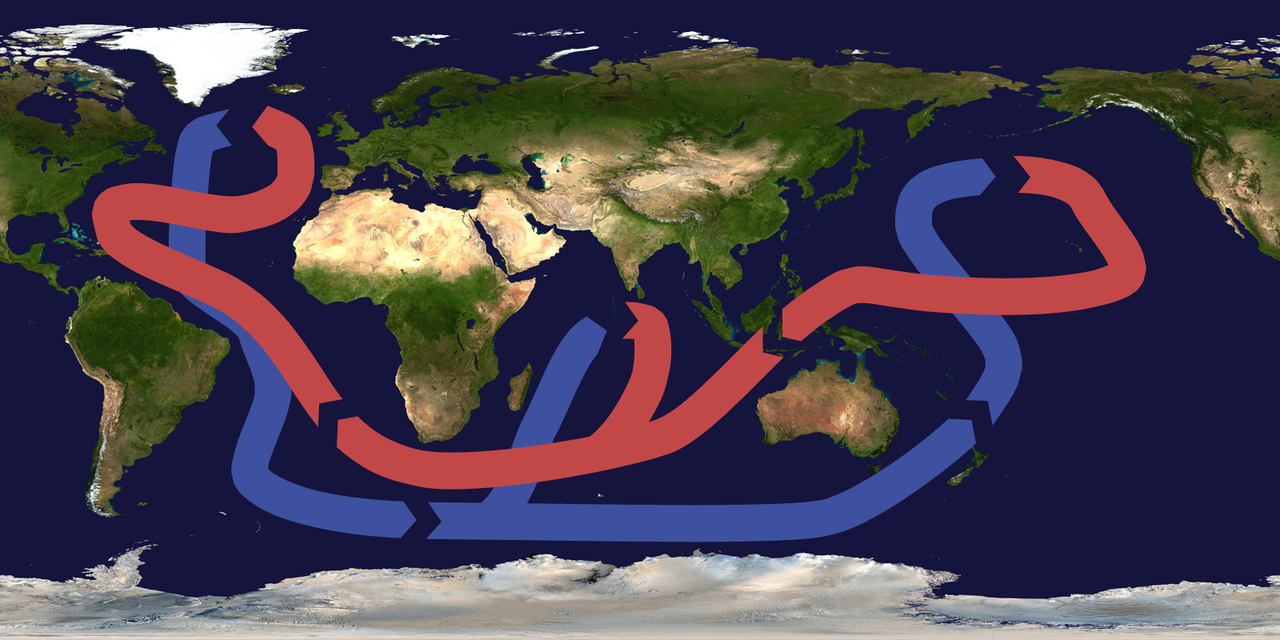
\includegraphics[width=\hsize]{chapters/4/1280px-Thermohaline_circulation.png}
\caption{
Das globale Förderband der thermohalinen Zirkulation.
\label{skript:thc:foerderband}}
\end{figure}%
Der Salzgehalt des Meerwassers ist nicht konstant,
hat aber ähnlich grossen Einfluss auf die Dichte wie die Temperatur.
Dies führt zu einer grossräumigen Zirkulationsströmung in den Weltmeeren,
genannt die thermohaline Zirkulation,
und damit zu einem weiteren bedeutenden Energietransportmechanismus.
Abbildung~\ref{skript:thc:foerderband} zeigt den Umfang der Zirkulation,
auch genannt das globale Förderband (conveyor belt).
Auf einer Zeitskala von Jahrzehnten bis Jahrhunderten wird Meerwasser 
und damit auch Wärmeenergie über Distanzen umgewälzt, welche mehrfach die
Erde umspannen.

Die Organismen, die in den oberen Wasserschichten absterben, sinken langsam
auf den Meeresgrund.
Ohne eine umfassende Umwälzung der Weltmeere würden die oberen Wasserschichten
mit der Zeit an Nährstoffen verarmen.
Die thermohaline Zirkulation stellt also auch die Versorgung der
Weltmeere mit Nährstoffen sicher.

Der Golfstrom ist ein kleiner Ausschnitt des globalen Förderbandes.
Die gut bekannte Bedeutung des Golfstroms für das europäische Klima 
deutet an, wie wichtig die thermohaline Zirkulation für das globale
Klima ist.
Es ist daher unerlässlich zu verstehen, was die Zirkulation antreibt und
wie sich der Klimawandel darauf auswirken könnte.

In diesem Kapitel soll die thermohaline Zirkulation modelliert werden.
Besonderes Augenmerk liegt dabei auf der Tatsache, dass dieses System
kippen kann.
Bei einer genügend grossen Änderung der Klimaparameter kann die Zirkulation
sich auf irreversible Art ändern.
Ein solches Ereignis hätte katastrophale Auswirkungen für das Klima.

%
% salinitaet.tex -- Salinität
%
% (c) 2018 Prof Dr Andreas Müller
%
\section{Salinität und Dichte}
\rhead{Salinität}
Der Salzgehalt des Meerwassers ist nicht konstant.
Er steigt an, wenn Wasser verdampf oder sich Eis bildet.
Er sinkt, wenn das Salz durch Niederschläge verdünnt wird.
Mit der Veränderung des Salzgehaltes geht auch eine Änderung
der Dichte einher.


%
% schichtung.tex -- Tiefenaufbau des Meeres
%
% (c) 2018 Prof Dr Andreas Müller, Hochschule Rapperswil
%
\section{Aufbau der Meere\label{section:thc:schichtung}}
\rhead{Aufbau der Meere}
\begin{figure}
\centering
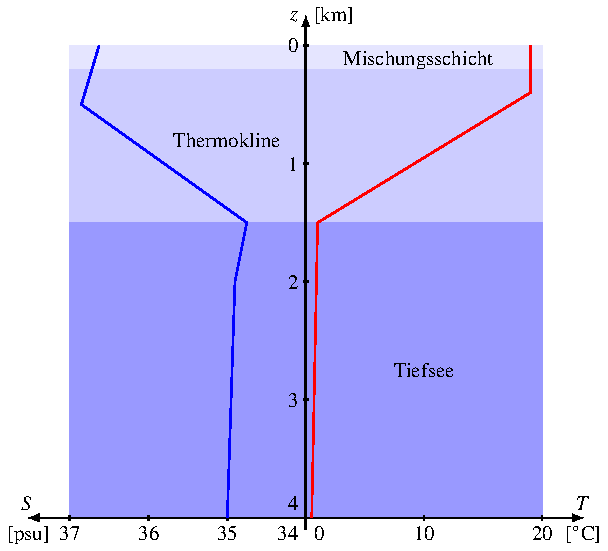
\includegraphics{chapters/4/schichten.pdf}
\caption{Tiefenaufbau des Meeres mit schematischem
Temperatur- und Salinitätsprofil.
Die Richtung der Achsen ist so gewählt, dass ``rechts'' gleichbedeutend
ist mit höher Dichte.
\label{skript:thc:schichtung}}
\end{figure}
Die Weltmeere umfassen etwa 1.4 Milliarden $\text{km}^3$ Wasser.
Wegen der hohen Wärmekapazität von $4.182\,\text{kJ}/\text{kg}\cdot\text{K}$
ist dies ein gigantisches Wärmereservoir mit entsprechend grosser
Bedeutung für das Klima.
Für das Verständnis des Klimassystems der Erde ist also die Kenntnis
des Aufbaus der Meere sowie des Energietransports in den Meeren unabdingbar.

Eine Reihe von Mechanismen beeinflussen Temperatur und Salinität.
An der Oberfläche wärmt sich das Wasser durch Einstrahlung
oder Zufluss warmen Wassers auf.
Wärmeaustausch mit der Atmosphäre gleicht die Temperatur von
Meer und Atmosphäre an, Verdunstung benötigt Energie und kühlt das Meer ab.
Der Zufluss von Süsswasser reduziert den Salzgehalt, die Verdungstung erhöht
die Salzkonzentration.
Durch Wind angeregte Turbulenz sorgt für gute Durchmischung dieser 
sogenannten {\em Mischungsschicht},
\index{Mischungsschicht}%
in ihr sind Temperatur und Salinität daher ungefähr konstant.
Sie reicht bis in eine Tiefe von wenigen hundert Metern.

In der Tiefe stehen bis auf einzelne wenige Stellen keine Quellen oder
Senken von Wärme oder Salz zur Verfügung.
Dort fehlt damit auch der Antrieb für Umwälzbewegungen, es bleibt
nur die Diffusion und die Schwerkraft.
Man kann daher davon ausgehen, dass in grosser Tiefe kaltes Wasser 
liegt mit weitgehend konstanter Temperatur und konstantem Salzgehalt.
Dies ist die {\em Tiefsee}.
\index{Tiefsee}%

Zwischen der Mischungsschicht und dem Tiefenwasser findet ein Ausgleich
von Temperatur und Salzgehalt statt.
Da dieser Ausgleich umso schneller erfolgt, je grösser der Unterschied
von Temperatur und Salinität erfolgt, ist ein Fliessgleichgewicht nur
möglich, wenn Temperatur und und Salinität in dieser Zone linear
von der Tiefe abhängen.
Diesen Bereich nennt man die {\em Thermokline}.
\index{Thermokline}%
Fehlt die Thermokline, hat das Oberflächenwasser die gleichen Eigenschaften
wie das Tiefenwasser, insbesondere gibt es keine Unterschiede, die eine
Umwälzung im Meer herbeiführen würden.
Je grösser tie Thermoklinentiefe, desto grösser auch der Unterschied
zwischen Obeflächenwasser und Tiefenwasser und desto mehr Energie für
den Antrieb der Zirkulation ist im Meer gespeichert.


%
% box.tex
%
% (c) 2018 Prof Dr Andreas Müller, Hochschule Rapperswil
%
\section{Ein Modell für die thermohaline Zirkulation}
\rhead{Ein Modell für die thermohaline Zirkulation}
Jedes numerische Modelle der Zirkulation basiert auf einer Diskretisation
des Gebietes.
Der Ozean wird also in kleine Teilgebiete aufgeteilt.
Gesucht sind Temperatur und Salinität in jedem Teilgebiet.
Dann werden Gleichungen aufgestellt, die den Austausch von Salz und
Wärme zwischen den Teilgebieten beschreiben.
Die Lösung dieser Gleichungen wird uns das Ausmass der Zirkulation zeigen
und erlauben abzuschätzen, wie sich die Zirkulation ändert, wenn sich
die äusseren Bedingungen verschieben.

\subsection{Ein einfaches Box-Modell}
Um einen ersten Eindruck von der Dynamik der thermohalinen Zirkulation
zu erhalten, verwenden wir ein Modell mit genau zwei Teilgebieten.
Wir modellieren den Atlantik nördlich des Äquators als zwei Gebiete.
Gebiet 1 ist das Polargebiet mit typischerweise tieferen Temperaturen,
Gebiet 2 ist das Gebiet in der Nähe des Äquators.
In jedem dieser Gebiet modellieren wir nur das Wasser, welches tatsächlich
von der Zirkulation umgewälzt wird.
Wir nehmen an, dass es sich durch die zwei Parameter Temperatur und
Salinität beschreiben lässt.
Wir bezeichnen die Variablen im Gebiet $i$ mit $T_i$ und $S_i$.

Das Wasser, welches an der Zirkulation teilnimmt, ist umgeben von einem
viel grösseren Wasserreservoir, welches mit dem strömenden Wasser 
im Wärme- und Salzaustausch steht.
Wir bezeichnen die konstanten Parameter dieser Reservoirs mit
$T_i^*$ und $S_i^*$.
In Abbildung~\ref{skript:boxmodell-bild} sind die beiden Gebiete
grau dargestellt, das in Zirkulation befindliche Wasser hellblau.
\begin{figure}
\centering
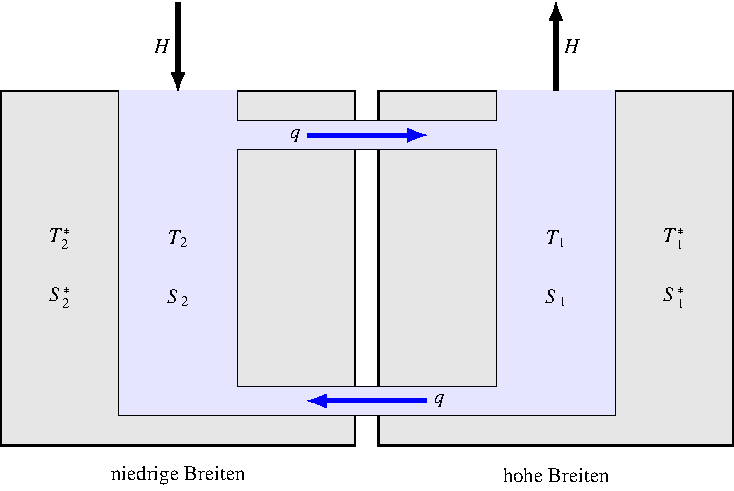
\includegraphics{chapters/4/boxmodell.pdf}
\caption{Einfaches Modell der thermohalinen Zirkulation
\label{skript:boxmodell-bild}}
\end{figure}

Die Zirkulation ist charakterisiert durch den Massefluss $q$ der
Tiefenströmung.
Da kein Wasser verloren gehen kann, muss in Oberflächennähe der gleiche
Fluss herrschen.
Da auch kein Salz verloren gehen kann, müssen sich auch die Salzflüsse
zwischen den beiden Gebieten ausgleichen.
Die Salinität wird zum Beispiel durch die Verdunstung erhöht, während
Niederschlag sie erniedrigt.
Süsswasserflüsse von Kontinenten reduzieren ebenfalls die Salinität.
Dies bedeutet, dass zusätzlich zum Massestrom $q$ ein virtueller 
Salzstrom zwischen den beiden Gebieten herrscht, den wir mit $H$ bezeichnen.

\subsection{Modell-Gleichungen\label{skript:thc:modell-gleichungen}}
Wir müssen jetzt Differentialgleichungen aufstellen, welche die
zeitliche Entwicklung von Temperatur $T_i(t)$ und Salinität $S_i(t)$
beschreiben kann.
Die Temperaturentwicklung wird bestimmt einerseits durch den Energietransport
durch den Fluss $q$ und andererseits durch den Wärmeaustausch mit dem
umgebenden Wasser.
Der Fluss $q$ hat zur Folge, dass sich die Temperaturen $T_1$ und $T_2$
angleichen.
Die beiden Flüsse oben und unten in Abbildung~\ref{skript:boxmodell-bild}
transportieren die gleiche Menge Wasser pro Zeiteinheit.
Es wird also gleichviel Wasser mit Temperatur $T_1$ ins Gebiet $2$ 
transportiert wie Wasser mit Temperatur $T_2$ ins Gebiet $1$.
Das Vorzeichen von $q$ spielt dabei keine Rolle, denn ändert das
Vorzeichen von $q$, fliesst das Wasser mit Temperatur $T_1$ einfach
durch den anderen Kanal.
Die Temperaturänderung von $T_1$ ist also proportional zu $|q|(T_2-T_1)$,
dies legt auch die Masseinheit von $q$ fest.

Der Wärmeaustausch mit dem umgebenden Wasser ist proportional zur
Temperaturdifferenz, wir bezeichnen den Proportionalitätsfaktor mit $c$.
Zusammen mit dem Wärmeaustausch durch die Strömung erhalten wir
die Differentialgleichungen
\begin{equation}
\begin{aligned}
\frac{dT_1}{dt}
&=
c(T_1^*-T_1)
+
|q|(T_2-T_1)
\\
\frac{dT_2}{dt}
&=
c(T_2^*-T_2)
+
|q|(T_1-T_2)
\end{aligned}
\label{skript:thc:temperaturgleichung}
\end{equation}
als Modell für die Temperaturentwicklung.

Analoge Überlegungen müssen wir jetzt auch noch für die Salinität anstellen.
Der Ausgleich der Salinität $S_i$ mit der Salinität $S_i^*$ des
umgebenden Meersbeckens ist proportional zur Differenz, der
Proportionalitätsfaktor, den wir mit $d$ bezeichnen, ist bestimmt durch
die Diffusionsgeschwindigkeit und die turbulente Durchmischung des
zirkulierenden Wassers mit der Umgebung.
Dazu kommt noch der virtuelle Salzfluss $H$:
\begin{equation}
\begin{aligned}
\frac{dS_1}{dt}
&=
\phantom{-}
H
+
d(S_1^*-S_1)
+
|q|(S_2-S_1)
\\
\frac{dS_2}{dt}
&=
-H
+
d(S_2^*-S_2)
+
|q|(S_1-S_2).
\end{aligned}
\label{skript:thc:salinitaetsgleichung}
\end{equation}
Man beachte, dass die Temperaturgleichungen~\eqref{skript:thc:temperaturgleichung}
und die Salinitätsgleichungen~\eqref{skript:thc:salinitaetsgleichung} 
gekoppelt sind, da der Fluss $q$ angetrieben wird vom Dichteunterschied,
der wiederum von Temperatur und Salinität abhängt.

\subsection{Antrieb der Zirkulation}
Die Zirkulation wird vom Dichteunterschied angetrieben.
Es gibt also einen Proportionalitätsfaktor $k$ derart, dass
\[
q = k\frac{\varrho_1 - \varrho_2}{\varrho_0}.
\]
Setzt man die Formel~\eqref{skript:salinity-linear} ein, findet man
\[
q
=
k(-\alpha(T_1-T_2) + \beta(S_1-S_2))
=
k(\alpha(T_2-T_1) + \beta(S_1-S_2))
=
k(\alpha(T_2-T_1) - \beta(S_2-S_1)).
\]
Schreiben wir $\Delta T = T_2-T_1$ und $\Delta S=S_2-S_1$,
dann ist der Fluss nur von den Differenzen abhängig:
\begin{equation}
q=k(\alpha\Delta T-\beta\Delta S).
\label{skript:thc:fluss-delta}
\end{equation}

\subsection{Anomalie-Gleichungen}
Die absoluten Werte von $T_i$ und $S_i$ sind nicht wirklich wichtig,
viel wichtiger sind die Unterschiede $\Delta T_i$ und $\Delta S_i$.
Verschwinden die Differenzen, kommt die Zirkulation zum erliegen,
und dies sind die Phänomene, die wir mit den Gleichungen prognostizieren
können möchten.
Wir streben daher an, die Gleichungen
\eqref{skript:thc:temperaturgleichung}
und
\eqref{skript:thc:salinitaetsgleichung}
in eine Form zu bringen, die nur von Differenzen und Anomalien
abhängt.

Wir schreiben
\[
T_0
=
\frac12(T_1+T_2)
\qquad\text{und}\qquad
S_0
=
\frac12(S_1+S_2)
\]
für die Mittelwerte von Temperatur und Salinität.
Indem wir den Mittelwert der Temperaturgleichungen
\eqref{skript:thc:temperaturgleichung}
bzw.~der Salinitätsgleichung \eqref{skript:thc:salinitaetsgleichung} bilden,
bekommen wir die Gleichungen
\begin{equation}
\begin{aligned}
\frac{dT_0}{dt}
&=
c(T_0^*-T_0)
\\
\frac{dS_0}{dt}
&=
d(S_0^*-S_0),
\end{aligned}
\label{skript:thc:mittelgleichung}
\end{equation}
wobei $T_0^* = \frac12(T_1^*+T_2^*)$ und $S_0^* = \frac12(S_1^*+S_2^*)$.
Die Differentialgleichungen~\eqref{skript:thc:mittelgleichung} 
besagen, dass die mittlere Temperatur des zirkulierenden Wassers
gegen die mittlere Temperatur des umliegenden Meeresbeckens strebt.
Die Faktoren $c$ und $d$ beschreiben, wie schnell der Temperaturausgleich
stattfindet, wie in Abschnitt~\ref{section:zeitkonstanten} ausgeführt wird.

Da die Mitteltemperatur langfristig gegen die Mitteltemperatur der
umliegenden Meeresbecken strebt, liegt es nahe, Temperatur und
Salinität auf diese Mitteltemperatur zu beziehen.
Wir ersetzen also
\begin{equation}
\begin{aligned}
\bar T_1&=T_1-T_0^*,
&
\bar T_2&=T_2-T_0^*
&&\Rightarrow&
\bar T_0&=T_0-T_0^*
\\
\bar S_1&=S_1-S_0^*,
&
\bar S_2&=S_2-S_0^*
&&\Rightarrow&
\bar S_0&=S_0-S_0^*
\end{aligned}
\end{equation}
Die Differentialgleichungen~\eqref{skript:thc:mittelgleichung}
für die Mittelwerte wird damit zu
\begin{align*}
\frac{d\bar T_0}{dt} &= -c \bar T_0\\
\frac{d\bar S_0}{dt} &= -d \bar S_0.
\end{align*}
Die Differentialgleichungen für
$T_i=\bar T_i + T_0^*$
und
$S_i=\bar S_i + S_0^*$
sind
\begin{align*}
\frac{dT_i}{dt}
&=
\frac{d\bar T_i}{dt}
=
c(T_i^*-T_i)
+ |q|\Delta \bar T
=
c(T_i^*- \bar T_i - T_0^*)
+ |q|\Delta \bar T
\\
\frac{dS_i}{dt}
&=
\frac{d\bar S_i}{dt}
=
\pm H
+
d(S_i^*-S_i)
+ |q|\Delta \bar S
=
\pm H
+
d(S_i^*- \bar S_i - S_0^*)
+ |q|\Delta \bar S
\end{align*}
Die Differenzen $T_i^*-T_0^*$ und $S_i^*-S_0^*$ können wir vereinfacht
als
\begin{align*}
T_1^*-T_0^* 
&=
T_1^* - \frac12(T_2^*-T_1^*)
=
-\frac12(T_2^*-T_1^*)
=
-T^*
\\
T_2^*-T_0^*
&=
T_2^*-\frac12(T_2^*-T_1^*)
=
\frac12(T_2^*-T_1^*)
=
T^*
\end{align*}
schreiben und analog für $S^*=\frac12(S_2^*-S_1^*)$.
Damit werden die Differentialgleichungen zu
\begin{equation}
\begin{aligned}
\frac{d\bar T_1}{dt}
&=
c(-T^*-\bar T_1) + |q| (\bar T_2-\bar T_1)
\\
\frac{d\bar T_2}{dt}
&=
c(T^*-\bar T_2) + |q| (\bar T_1-\bar T_2)
\\
\frac{d\bar S_1}{dt}
&=
-H
+
d(-S^*-\bar S_1) + |q|(\bar S_2 - \bar S_1)
\\
\frac{d\bar S_2}{dt}
&=
\phantom{-}H
+
d(S^*-\bar S_2) + |q|(\bar S_1 - \bar S_2)
\end{aligned}
\label{skript:thc:anomaliegleichungen}
\end{equation}
Man beachte, dass die $T^*$ und $S^*$ konstant sind.

In den Gleichungen~\eqref{skript:thc:anomaliegleichungen} hängt
$q$ von den Temperatur- und Salinitätsdifferenzen ab.
Wegen $\Delta\bar T=\Delta T$ und $\Delta\bar S=\Delta S$ ist nach
\eqref{skript:thc:fluss-delta}
\begin{equation}
q = k(\alpha\Delta\bar T-\beta \Delta\bar S).
\label{skript:thc:fluss-delta-anomalie}
\end{equation}

\subsection{Differenzgleichungen}
Wir können die Anomaliegleichungen \eqref{skript:thc:anomaliegleichungen}
noch etwas weiter umformen und die einzelnen Ano\-malien vollständig durch
die Differenzen ersetzen.
Die Differenzen und Summen der Gleichungen sind
\begin{equation}
\begin{aligned}
\frac{d\Delta\bar T}{dt}
&=
c(2T^*-\Delta\bar T)-2|q|\Delta\bar T
&&\qquad&
\frac{d\bar T_0}{dt}
&=
-c\bar T_0
\\
\frac{d\Delta\bar S}{dt}
&=
2H+d(2S^*-\Delta\bar S) - 2|q|\Delta\bar S
&&\qquad&
\frac{d\bar S_0}{dt}
&=
-d\bar S_0.
\end{aligned}
\label{skript:thc:differenzgleichungen}
\end{equation}
Die Gleichungen rechts drücken aus, dass die mittleren Anomalien
exponentiell gegen $0$ gehen.
Die linken Gleichungen beschreiben die Zeitentwicklung der Differenz
der Anomalien.
Man beachte, dass $q$ ebenfalls von den Anomalie-Differenzen abhängt.

\subsection{Zeitkonstanten\label{section:zeitkonstanten}}
\label{skript:thc:zeitkonstanten}
Der Koeffizienten $c$ beschreibt, wie schnell der Temperaturausgleich
durch Wärmeleitung oder turbulente Durchmischung erfolgt.
Der Koeffizient $d$ beschreibt, wie schnell der Salinitätsausgleich
durch Durchmischung und Diffusion stattfinden kann.
Je grösser diese Koeffizienten, desto schneller erfolgt der Prozess.
In den rechten Gleichungen von \eqref{skript:thc:differenzgleichungen}
ist dies ganz offensichtlich.
Vernachlässigen wir für den Moment den Einfluss der Zirkulation,
was wir durch $k=0$ im Ausdruck für $q$ beschreiben können, dann
sehen wir, dass die Differenzgleichungen beide von der Form
einer linearen inhomogenen Differentialgleichung
\[
\frac{d\Delta X}{dt}
=
X^* -cX
\]
sind, wobei $X^*$ eine Konstante ist.
Die Lösung der Gleichung ist
\[
X(t) = \frac{X^*}{c} + C_0 e^{-ct}
\]
mit einer Konstanten $C_0$, die aus den Anfangsbedingungen zu
bestimmen ist.
Die Terme $T^*$, $S^*$ und $H$ verschieben also nur die Lösung,
die Differenzen $\Delta\bar T$ und $\Delta\bar S$ streben exponentiell
wie $e^{-ct}$ bzw.~$e^{-dt}$ gegen diese Gleichgewichtswerte.

Die Grössen $1/c$ und $1/d$ haben die Dimension einer Zeit, wir nennen
sie die {\em Zeitkonstanten} des Prozesses, den $c$ bzw.~$d$ beschreiben.
\index{Zeitkonstante}
Ist zum Beispiel die Zeitkonstante $1/c$ der Temperatur sehr viel kleiner
als die Zeitkonstanten $1/d$ der Salinität, dann bedeutet dies, dass
sich die Temperaturdifferenzen sehr viel schneller ausgleichen als die
Salinitätsdifferenzen.
Für die langfristige Entwicklung der Zirkulation ist in diesem Fall
die Salinitätsentwicklung ausschlaggebend, die Temperaturfunktionen
können durch Konstanten ersetzt werden.





%
% dimensionslos.tex
%
% (c) 2018 Prof Dr Andreas Müller, Hochschule Rapperswil
%
\section{Dynamik der thermohalinen Zirkulation}
\rhead{Dynamik der thermohalinen Zirkulation}
In diesem Abschnitt wollen wir die
Bewegungsgleichung~\eqref{skript:thc:differenzgleichungen}
etwas vereinfachen mit dem Ziel, einzelne Szenarien durchspielen
zu können.
Eine vertiefte Diskussion solcher Modelle ist in
Kapitel~\ref{chapter:thermohalin} zu finden.

\subsection{Elimination von Prozessen mit kurzer Zeitkonstante}
Die Diskussion in Abschnitt~\ref{skript:thc:zeitkonstanten}
ist es zulässig, Variablen mit sehr kleiner Zeitkonstanten
durch Konstanten zu ersetzen.
Tatsächlich erfolgt der Temperaturausgleich im Wasser sehr viel
schneller als der Salinitätsausgleich.
Wir können daher davon ausgehen, dass die Temperaturgleichungen
die Temperaturanomalien sehr schnell gegen eine Gleichgewichtstemperatur
streben lassen und dass wir für die Lösung der Salinitätsgleichungen
mit dieser konstanten Temperatur arbeiten können.

Wir gehen also davon aus, dass $\Delta\bar T=2T^*$ konstant ist und
reduzieren damit das Gleichungssystem
\eqref{skript:thc:differenzgleichungen}
auf die eine Gleichung
\begin{equation}
\frac{d}{dt}\Delta\bar S
=
2H + d(2S^* -\Delta\bar S) - 2|q|\Delta\bar S
\qquad\text{mit}\qquad
q=k(2\alpha T^* -\beta \Delta\bar S).
\label{skript:thc:salinitaetallein}
\end{equation}
Diese Gleichungen beschreiben also die Salinitätsentwicklung unter
der Annahme, dass der Temperaturausgleich sehr schnell erfolgt.
Dieser Ausgleich kann nicht primär durch Durchmischung erfolgen,
denn dieser Mechanimus würde auch die Salinität mit gleicher
vergleichbarer Geschwindigkeit ausgleichen.
Dies bedeutet, dass der dominante Term in der Temperaturgleichung
der Term mit $c$ ist, nicht der Term mit $q$.

Die Gleichung \eqref{skript:thc:salinitaetallein} kann noch nicht auf
einfache Weise gelöst werden.
Wir vereinfachen wir sie daher weiter indem wir ausnutzen, dass 
der Salinitätsausgleich so viel langsamer ist als der Temperaturausgleich,
dass der Term mit $d$ im Vergleich zum Term mit $q$ vernachlässigbar ist.
Wir setzen also $d=0$ und
erhalten damit 
\begin{equation}
\frac{d}{dt}\Delta\bar S
=
2H - 2|q|\Delta\bar S
\qquad\text{mit}\qquad
q=k(2\alpha T^* -\beta \Delta\bar S)
\label{skript:thc:qgleichung}
\end{equation}
als vereinfachte Differentialgleichung zur Modellierung der 
thermohalinen Zirkulation.
Dies ist eine nichtlineare Differentialgleichung erster Ordnung,
die nicht in geschlossener Form gelöst werden kann.

\subsection{Eine dimensionslose Beschreibung}
Die Gleichung \eqref{skript:thc:qgleichung} ist wegen der vielen
Konstanten unübersichtlich.
Ausgeschrieben lautet sie
\begin{equation}
\frac{d}{dt}\Delta\bar S
=
2H
-2k\,|\alpha\Delta\bar T- \beta \Delta\bar S|\,\Delta\bar S
\label{skript:thc:smitdim}
\end{equation}
Die meisten der Konstanten können wir aber los werden, indem wir 
die unabhängigen Variablen und die Zeit neu skalieren.
Dies ist gleichbedeutend mit einem Wechsel der Masseinheiten.
Wir verwenden:
\begin{equation}
x=\frac{\beta\Delta\bar S}{\alpha\Delta\bar T},
\qquad
\tau = 2\alpha k\,|\Delta\bar T|\, t
\qquad\text{und}\qquad
\lambda = \frac{\beta H}{\alpha^2 k\Delta\bar T|\Delta\bar T|}.
\label{skript:thc:masseinheiten}
\end{equation}
Die Ableitung nach $t$ kann durch die Ableitung nach $\tau$ ausgedrücket
werden vermöge der Ersetzung
\[
\frac{d}{d\tau}
=
\frac{1}{2\alpha k|\Delta\bar T|}
\frac{d}{dt}
\qquad\Rightarrow\qquad
\frac{d}{dt}
=
2\alpha k|\Delta\bar T|\frac{d}{d\tau}.
\]
Setzen wir dies in die Gleichung~\eqref{skript:thc:masseinheiten}
ein, erhalten wir
\begin{equation}
2\alpha k|\Delta\bar T|
\frac{d}{d\tau} \Delta\bar S
=
2H-2k|\alpha\Delta\bar T-\beta\Delta\bar S|\,\Delta\bar S.
\end{equation}
Wir erweitern mit $\beta/\alpha\Delta\bar T$, damit wird die
Differentialgleichung zu
\begin{align}
2\alpha k|\Delta\bar T|
\frac{d}{d\tau}\frac{\beta\Delta\bar S}{\alpha\Delta\bar T}
&=
\frac{2\beta H}{\alpha\Delta\bar T} - 2k|\alpha\Delta\bar T-\beta\Delta\bar S|\,
\frac{\beta\Delta\bar S}{\alpha\Delta\bar T}
\notag
\\
\alpha k|\Delta\bar T|
\frac{d}{d\tau}x
&=
\frac{\beta H}{\alpha\Delta\bar T}
-k|\alpha\Delta\bar T-\beta\Delta\bar S|\, x
\notag
\\
k
\frac{d}{d\tau}x
&=
\frac{\beta H}{\alpha^2\Delta\bar T\,|\Delta\bar T|}
-k\biggl|1-\frac{\beta\Delta\bar S}{\alpha\Delta\bar T}\biggr|\,x
\notag
\\
\frac{d}{d\tau}x
&=
\frac{\beta H}{k\alpha^2\Delta\bar T\,|\Delta\bar T|}
-\biggl|1-\frac{\beta\Delta\bar S}{\alpha\Delta\bar T}\biggr|\,x
\notag
\\
\frac{dx}{d\tau}
&=
\lambda - |1-x|x.
\label{skript:thc:dimensionslos}
\end{align}
Damit haben wir die ursprüngliche Gleichung
\eqref{skript:thc:smitdim}
in eine dimensionslose Gleichung mit dem einen Parameter $\lambda$
umgewandelt.
%Das Verhalten der Lösung hängt vom Parameter $\lambda$ ab.

\subsection{Gleichgewicht}
Um das Verhalten der Lösungen von 
\eqref{skript:thc:dimensionslos}
besser zu verstehen, suchen wir zunächst nach Gleichgewichtslösungen.
Diese hängen nicht von der Zeit ab, es gilt also
\begin{equation}
\frac{dx}{d\tau}=0
\qquad\Rightarrow\qquad
\lambda-|1-x|x=0
\qquad\Rightarrow\qquad
|1-x|x
=
\lambda.
\label{skript:thc:lambdagl}
\end{equation}
\begin{figure}
\centering
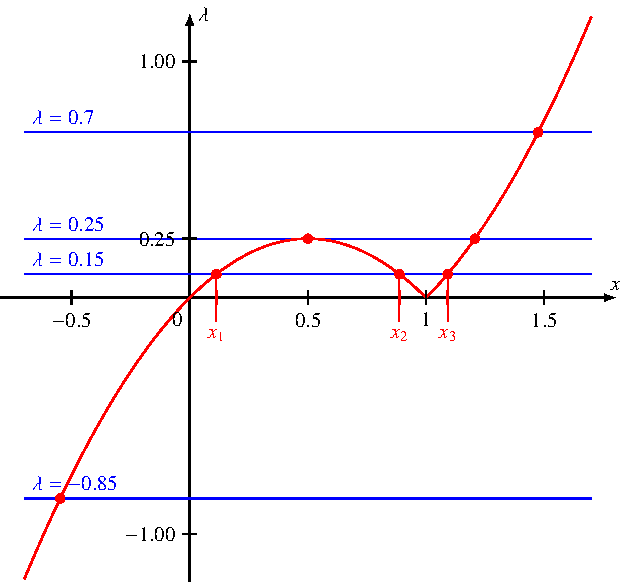
\includegraphics{chapters/4/rhs.pdf}
\caption{Graph der Funktion $|1-x|\,x$ und
Gleichgewichtslösungen der dimensionslosen Differentialgleichung
\eqref{skript:thc:dimensionslos}
\label{skript:thc:1-xxgraph}}
\end{figure}%
In Abbildung~\ref{skript:thc:1-xxgraph} ist der Graph der Funktion 
$|1-x|\,x$ dargestellt.
Je nach dem Wert von $\lambda$ hat die dimensionslose Differentialgleichung
\eqref{skript:thc:dimensionslos} bis zu drei Gleichgewichtslösungen.

Für Werte von $\lambda$ zwischen $0$ und $0.25$ gibt es drei verschiedene
Werte $x$, die die Gleichung \eqref{skript:thc:lambdagl} erfüllen
(Abbildung~\ref{skript:thc:drei}).
Für $x\le 1$  ist $1-x\ge 0$ und damit muss $x$ die 
Gleichung $(1-x)x=\lambda$ erfüllen, für $x\ge 1$ ist es die Gleichung
$(x-1)x=\lambda$.
Diese beiden Gleichungen haben die folgenden Lösungen
\begin{align*}
&\text{Fall $x \le 1$:}
&
(1-x)x&=\lambda
&
&\text{Fall $x\ge 1$:}
&
(x-1)x&=\lambda
\\
&&
x^2-x+\lambda&=0
&&&
x^2-x-\lambda&=0
\\
&&
x&=\frac12\pm\sqrt{\frac14-\lambda}
&&&
x&=\frac12+\sqrt{\frac14+\lambda}.
\end{align*}
Die rechte Gleichung hat für alle Werte $\lambda > 0$ zwar auch noch
eine Lösung $<1$, diese ist aber ausgeschlossen, daher nur das
positive Zeichen vor der Wurzel in diesem Fall.
Für $\lambda > 0.25$ hat die linke Gleichung keine Lösung.
Für $\lambda < 0$ ist die Lösung mit dem positiven Zeichen der linken
Gleichung ausgeschlossen.

\begin{figure}
\centering
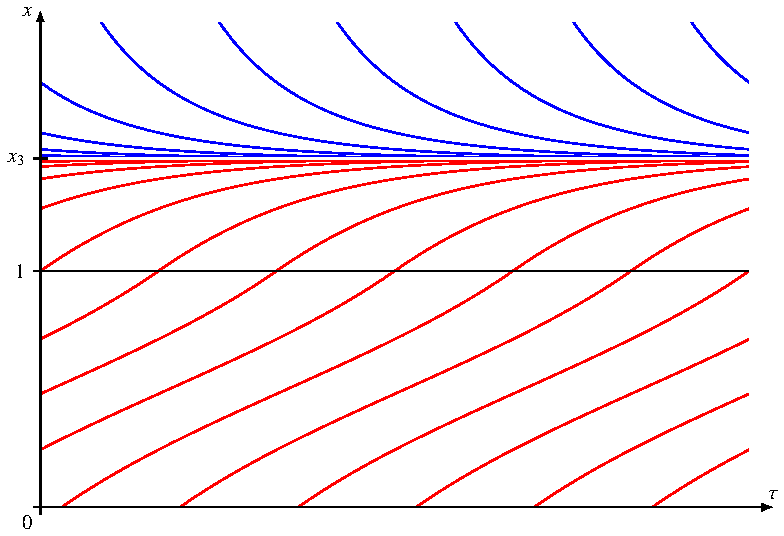
\includegraphics{chapters/4/ein.pdf}
\caption{Lösungen im Fall $\lambda > \frac14$: der einzige
Gleichgewichtspunkt $x_3$ ist stabil.
\label{skript:thc:ein}}
\end{figure}%
Wir berechnen die Lösung der Differentialgleichung für einen gegebenen
Wert von $\lambda$ (Abbildung~\ref{skript:thc:ein}).
Für $\lambda >\frac14$ gibt es nur einen Gleichgewichtspunkt, wir 
nennen ihn $x_3$.
Falls $x(\tau)<x_3$, dann ist
\[
\frac{dx}{d\tau}
=
\lambda - |1-x|x > 0,
\]
die Lösung $x(\tau)$ ist also monoton wachsend.
Für $x(\tau) > x_3$ ist hingegen
\[
\frac{dx}{d\tau}
=
\lambda - |1-x|x < 0,
\]
die Lösung ist also monoton fallend.
Lösungskurven, die bei $x$-Werten $>x_3$ beginnen nehmen monoton ab
und konvergieren gegen $x_3$, solche, die bei $x$-Werten $<x_3$ beginnen,
nehmen monoton zu und konvergieren von unten gegen $x_3$.
Die Gleichgewichtslösung $x(\tau)=x_3$ ist also eine stabile Lösung,
alle anderen Lösungen konvergieren gegen diese Lösung.

\begin{figure}
\centering
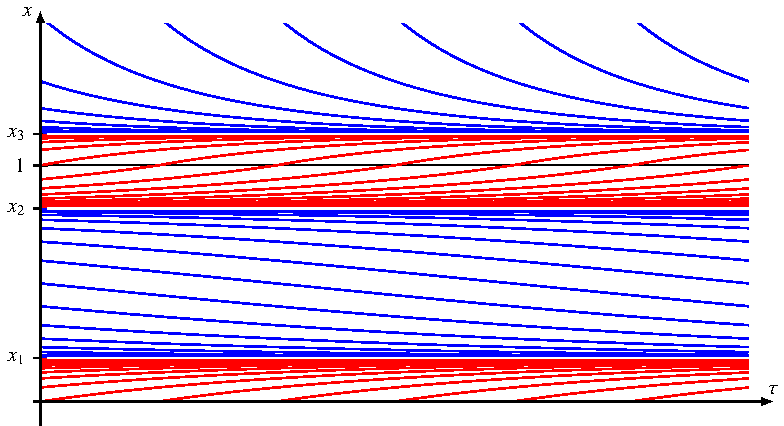
\includegraphics{chapters/4/drei.pdf}
\caption{Lösungen im Fall $0\le \lambda\le\frac14$: die beiden
Gleichgewichtspunkte $x_1$ und $x_3$ sind stabil, $x_2$ ist instabil.
\label{skript:thc:drei}}
\end{figure}%
Für $0<\lambda<\frac14$ seien
$x_1$, $x_2$ und $x_3$ die drei Gleichgewichtspunkte
(Abbildung~\ref{skript:thc:drei}).
Wir untersuchen wieder die Vorzeichen von $dx/d\tau$. 
Für $x$-Werten zwischen $x_1$ und $x_2$ und für $x$-Werte grösser
als $x_3$ ist die Ableitung positiv, die Lösungen konvergieren monoton
wachsend gegen die Gleichgewichtslösungen $x_1$ bzw.~$x_3$.
Lösungen, die bei $x<x_1$ oder $x_2<x<x_3$ beginnen, konvergieren
dagegen monoton wachsend gegen $x_1$ bzw.~$x_3$.
Die Gleichgewichtslösung $x_2$ ist daher nicht stabil,
die Gleichgewichtslösungen $x_1$ und $x_3$ sind dagegen stabil.

\subsection{Bifurkation}
In diesem Abschnitt studieren wir die Abhängigkeit der Gleichgewichtslösungen
in Abhängigkeit vom Parameter $\lambda$, wie dies in Abschnitt
\ref{section:bifurkation-eindim} vorbereitet wurde.

\begin{figure}
\centering
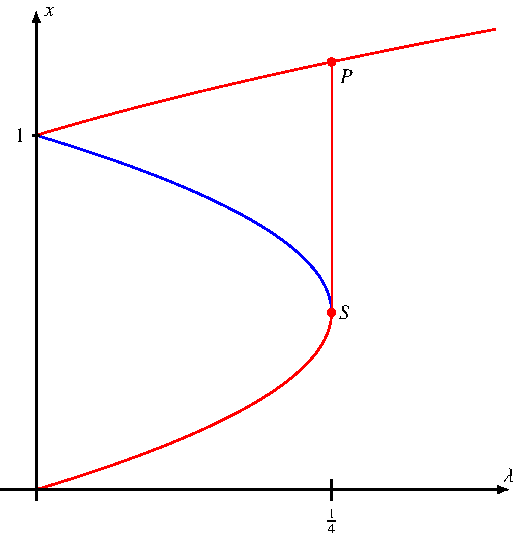
\includegraphics{chapters/4/bi.pdf}
\caption{Bifurkationsdiagramm für die Differentialgleichung
\eqref{skript:thc:lambdagl}
\label{skript:thc:bifurkation}}
\end{figure}
Für Parameterwerte $\lambda < \frac14$ gibt es drei mögliche
Gleichgewichtspunkte, für $\lambda>\frac14$ jedoch nur noch einen.
Wir möchten untersuchen, wie sich die Lösung verhält, wenn der
Parameter langsam verändert wird.
Dies ist in Abbildung~\ref{skript:thc:bifurkation} dargestellt.

Sei jetzt also zunächst $\lambda <\frac14$.
Wir betrachten eine Lösung, die in Nähe von
\[
x_1(\lambda)=\frac12-\sqrt{\frac14-\lambda}
\]
beginnt.
Vergrössern wir $\lambda$, verschiebt sich der Gleichgewichtspunkt
$x_1(\lambda)$ ebenfalls nach oben.
Da $x_1(\lambda)$ aber ein stabiler Gleichgewichtspunkt ist, wird die
Lösung gegen den neuen Gleichgewichtspunkt konvergieren.
Das gleiche passiert auch, wenn die Lösung in der Nähe von
\[
x_3(\lambda)=\frac12+\sqrt{\frac14+\lambda}
\]
beginnt.
Bei einer Vergrösserung folgt das System den roten Kurven in
Abbildung~\ref{skript:thc:bifurkation}.

Wenn jetzt aber der Parameter $\lambda$ die Schwelle $\frac14$
überschreitet, dann wird die Lösung zum einzigen verbleibenden
stabilen Gleichgewichtspunkt $x_3(\lambda)$ konvergieren.
Die Lösung springt also vom Punkt $S$ zum Punkt $P$ auf dem oberen roten Ast
in Abbildung~\ref{skript:thc:bifurkation}.

Wenn man den Parameter $\lambda$ wieder verkleinert, dann wird
eine Lösung in der Nähe von $x_3(\lambda)$ wieder gegen
$x_3(\lambda)$ konvergieren.
Es ist aber nicht mehr möglich, dass die Lösung gegen $x_1(\lambda)$
konvergiert, da nach Abbildung~\ref{skript:thc:drei} nur Lösungen,
die bei $x$-Werten $<x_2$ beginnen, gegen $x_1(\lambda)$ konvergieren
können.

Dieses einfache Modell der thermohalinen Zirkulation hat also die
überraschende Eigenschaft, dass das System beim Überschreiten des
kritischen Wertes $\lambda=\frac14$ in einen Zustand kippt, aus dem
es nicht mehr zurück kommen kann.
Wegen
\[
\lambda
=
\frac{\beta H}{\alpha^2k\Delta\bar T\,|\Delta\bar T|}
\]
kann dies passieren wenn entweder der Betrag des virtuellen Salzflusses 
$H$ ansteigt oder die Temperaturanomaliedifferenz $\Delta\bar T$
klein wird.
Eine Klimaerwärmung könnte zum Beispiel die Verdunstung im Gebiet $2$
erhöhen, den virtuellen Salzfluss erhöhen und damit das System
in den Zustand mit einer wesentlich grösseren Anomaliedifferenz
$\Delta\bar S$ kippen lassen.










%
% zonen.tex -- Zonenmodelle für das Klima
%
% (c) 2018 Prof Dr Andreas Müller, Hochschule Rapperswil
%
\chapter{Zonenmodelle\label{chapter:zonenmodelle}}
\lhead{Kapitel \thechapter: Zonenmodelle}
Die Erdrotation ist schnell im Vergleich zu den für typische Klimamodelle
wesentlichen Zeitspannen.
Wesentliche Aspekte der Klimaentwicklung sollten sich daher immer
noch modellieren lassen, wenn man den Zustand des Klimasystems über
die Erdrotation mittelt.
In diesem Kapitel werden daher vereinfachte Modelle diskutiert,
die nur die geographischen Länge als geometrischen Parameter haben.

%
% strahlung.tex
%
% (c) 2018 Prof Dr Andreas Müller, Hochschule Rapperswil
%
\section{Strahlung\label{section:strahlung}}
\rhead{Strahlung}
Die von der Erde empfange Strahlung sowie die Albedo wurden bereits in
Abschnitt~\ref{skript:grundlagen:strahlung} untersucht.
Für die später in diesem Kapitel zu untersuchenden Modelle ist aber
erforderlich, die örtliche Verteilung der Strahlung auf der Erdoberfläche
genauer zu verstehen.
In diesem Abschnitt wird daher zuerst die Strahlungsleistung auf einer
Halbkugel und später auf einer Zone um einen Breitenkreis berechnet.
\input{chapters/5/halbkugel.tex}
\input{chapters/5/einstrahlung.tex}

%
% bilanz.tex -- Bilanz-Modelle
%
% (c) 2018 Prof Dr Andreas Müller, Hochschule Rapperswil
%
\section{Strahlungsbilanzmodelle\label{skript:section:budyko}}
\rhead{Strahlunbsbilanzmodelle}
Im Kapitel~\ref{chapter:wetter und klima} haben wir die physikalischen
Grundlagen der Wetter und Klimaphänomene studiert.
In diesem Abschnitt wollen wir ein einfaches Modell für die Energiebilanz
der Erde entwickeln.

\subsection{Strahlungsbilanz\label{skript:subsection:strahlungsbilanz}}
Wir formulieren ein Modell mit einer einzigen Variablen, der globalen
Mitteltemperatur $T$.
Berechnet werden soll die zeitliche Entwicklung von $T$.

\subsubsection{Einstrahlung}
Die Erde mit Radius $R$ erhält ihre Energie von der Sonne, die
den konstanten Energiefluss $S_0 = 1368 \text{W\,m}^{-2}$
einstrahlt.
Der Querschnitt der Erde ist $\pi R^2$, auf den eine Leistung von
$\pi R^2 S_0$ fällt.
Die Atmosphäre und die Weltmeere transportieren diese Energie, wir nehmen
an, sie gleichmässig über die ganze Erdoberfläche verteilt wird.
Die pro Flächeneinheit anfallende Leistung ist daher
\begin{equation}
\frac{\pi R^2 S_0}{4\pi R^2} = \frac14S_0=Q.
\label{skript:bilanz:einstrahlung}
\end{equation}

Doch kann nicht die gesamte Energie absorbiert werden.
Ein Teil wird von Wolken oder von Eis an der Oberfläche 
gleich wieder reflektiert, aber auch Landmassen und die Meere reflektieren
einen kleineren Teil der Strahlung.
Die auf Seite~\pageref{skript:subsubsection:albedo} beschriebene Albedo
hat für die Erde Werte zwischen $0.3$ und $0.7$ je nach dem Grad der
Bewölkung und der Vereisung.
Bei tieferer Temperatur muss mit stärkerer Vereisung und mehr Wolken
gerechnet werden.
Sei $\alpha(T)$ die Albedo der Erde bei der Temperatur $T$.
Der von der Erde absorbierte Fluss ist daher
\begin{equation}
(1-\alpha(T)) Q.
\label{skript:bilanz:ausstrahlung}
\end{equation}
Die Grösse $1-\alpha(T)$ heisst auch die {\em Coalbedo}.
\index{Coalbedo}%

\subsubsection{Ausstrahlung}
Die Erde verliert Energie auch wieder durch Strahlung.
Nach dem Stefan-Boltzmannschen Gesetz~\eqref{skript:stefon-boltzmann}
ist die Ausstrahlung der Erde proportional zur vierten Potenz der
Temperatur, also $T^4$.

\subsubsection{Bilanzgleichung}
Die Temperatur ändert sich umso mehr, je grösser das Ungleichgewicht
zwischen Einstrahlung \eqref{skript:bilanz:einstrahlung} und
\eqref{skript:bilanz:ausstrahlung} ist.
Die Wärmekapazität der Erdoberfläche spielt ebenfalls
eine Rolle, je grösser diese ist, desto träger folgt die Temperatur dem
Energiebilanzüberschuss.

Wir erhalten so die Differentialgleichung
\begin{equation}
C\frac{dT}{dt}
=
(1-\alpha(T)) Q - \sigma T^4.
\label{skript:bilanz:basic}
\end{equation}
Je grösser $C$ ist, desto kleiner ist die Änderungsgeschwindigkeit der
globalen Mitteltemperatur bei gleicher rechter Seite.

\subsubsection{Gleichgewichtslösung}
Wir suchen eine Gleichgewichtslösung für dieses Modell, und nehmen zu diesem
Zweck den typischen Wert $\alpha=0.3$ der Albedo der Erde.
Sie muss $\dot T=0$ erfüllen, also
\begin{align*}
(1-\alpha) Q -\sigma T^4 &=0
\\
\Rightarrow
\qquad
T&=\root 4\of{\frac{(1-\alpha)Q}{\sigma}}
\end{align*}
Setzt man die üblichen Werte für $Q$ ein, erhält man eine globale
Mitteltemperatur von $T=254.8\,\text{K}$.

\subsubsection{Treibhauseffekt}
Die tatsächliche global Mitteltemperatur $T=287.7\,\text{K}$ ist.
Diese Diskrepanz ist zwei Unzulänglichkeiten diesen einfachen
Modells zurückzuführen:
\begin{enumerate}
\item
Der Treibhauseffekt sorgt dafür, dass nur ein Teil der abgestrahlten
Wärmestrahlung die Erde tatsächlich verlässt.
Wir können dies dadurch modellieren, dass wir in der Gleichung
\eqref{skript:bilanz:basic} den Ausstrahlungsterm um einen Faktor
$\varepsilon$ reduzieren, der den Treibhauseffekt modellieren soll.
Die neue Grundgleichung wird dann
\begin{equation}
C\frac{dT}{dt}
=
(1-\alpha(T)) Q - \varepsilon\sigma T^4.
\label{skript:bilanz:basic2}
\end{equation}
Um die aktuelle Gleichgewichtstemperatur $T=287.7\,\text{K}$ von 2010
zu reproduzieren müssen wir $\varepsilon=0.32$ wählen.
\item
Die Albedo hängt von der Temperatur ab und wird mit abnehmender 
Temperatur grösser.
Bei sehr tiefen Temperaturen kann die Albedo auf bis $0.7$ steigen.
Ein einfaches Modell, welches Diesen Sachverhalt abbildet, ist
\begin{equation}
\alpha(T)=0.5-0.2\tanh\biggl(\frac{T-265}{10}\biggr)
\label{skript:bilanz:albedo}
\end{equation}
\end{enumerate}

\subsubsection{Gleichgewichte}
\begin{figure}
\centering
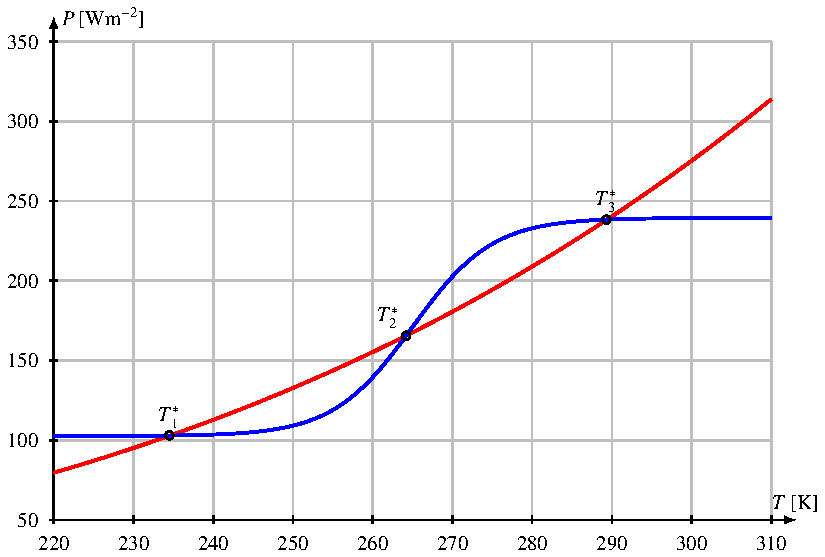
\includegraphics{chapters/5/bilanzmodell.pdf}
\caption{Einstrahlung und Ausstrahlung in dem einfachen Bilanzmodell
mit der Modellgleichung
\eqref{skript:bilanz:basic2} und der Albedo-Funktion
\eqref{skript:bilanz:albedo}.
Die Ausstrahlung $\varepsilon\sigma T^4$ ist rot eingezeichnet,
blau ist die Ausstrahlung.
Es entstehen drei Gleichgewichtspunkte $T_1^*$, $T_2^2*$ und $T_3^*$,
von denen aber $T_2^*$ nicht stabil ist.
\label{skript:bilanz:modellbild}}
\end{figure}
Das Modell mit der Albedo-Funktion~\eqref{skript:bilanz:albedo}
hat nicht nur einen sondern drei Gleichgewichtspunkte.
Die Einstrahlung und die Ausstrahlung ist in
Abbildung~\ref{skript:bilanz:modellbild} dargestellt.

Die beiden Gleichgewichtspunkte $T_1^*$ und $T_3^*$ sind stabil.
In beiden Punkten ändert sich die absorbierte Energie kaum bei
einer Temperaturänderung, aber die Ausstrahlung wird bei erhöhter 
Temperatur wesentlich effizienter, so dass sich die Erde wieder
abkühlt.
Ebenso verringert sich die Ausstrahlung bei leicht tieferer Temperatur
sofort, so dass die Erde sich wieder zur Gleichgewichtstemperatur aufwärmen
kann.

Das Gleichgewicht $T_2^*$ ist dagegen nicht stabil.
Bei höherer Temperatur wird die Einstrahlung sofort grösser, ohne dass
die Ausstrahlung mithalten kann, so dass sich die Erde weiter
aufwärmt bis zur Temperatur $T_3^*$.
Bei leicht tieferer Temperatur steigt die Albedo stark an so dass die
Einstrahlung schnell abnimmt, während die Ausstrahlung nur vergleichsweise
langsam zurückgeht, die Erde kühlt sich bis auf die Temperatur $T_1^*$ ab.

\subsubsection{Bifurkation und globale Erwärmung}
\begin{figure}
\centering
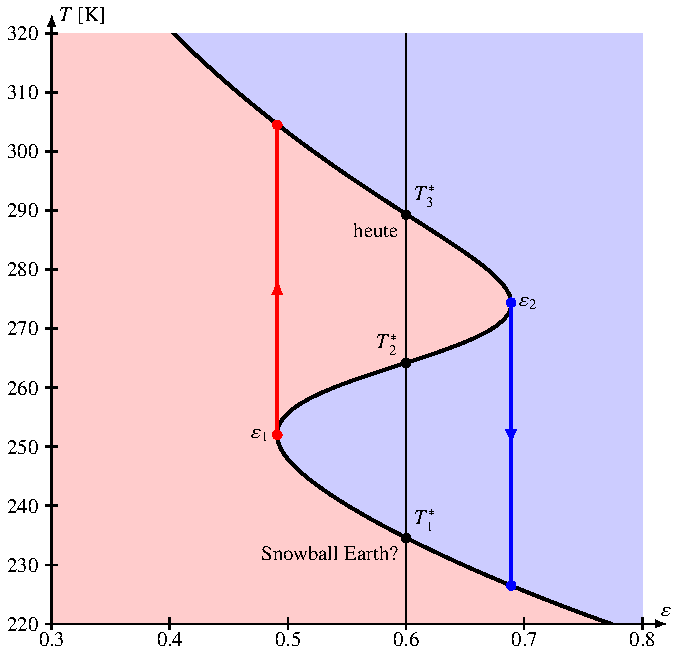
\includegraphics{chapters/5/bifurkation.pdf}
\caption{Bifurkationsdiagramm für das Bilanzmodell
\eqref{skript:bilanz:basic2}
in Abhängigkeit vom Treibhauseffekt-Parameter $\varepsilon$.
\label{skript:bilanz:bifurkation}}
\end{figure}
Der Parameter $\varepsilon$ modelliert den Treibhauseffekt.
Steigt die Konzentration der Klimagase in der Atmosphäre, wird die
abgestrahlten Leistung geringer, also $\varepsilon$ kleiner.
Es lohnt sich daher, die Entwicklung des Gleichgewichtspunkte in 
Abhängigkeit von $\varepsilon$ zu untersuchen.
Das Bifurkationsdiagramm des Modells
\eqref{skript:bilanz:basic2} in Abhängigkeit von $\varepsilon$
ist in Abbildung~\ref{skript:bilanz:bifurkation} dargestellt.

Man kann aus dem Diagramm ablesen, dass mit weitterer Zunahme des 
Treibhauseffektes, als mit Abnahme von $\varepsilon$, die globale
Mitteltemperatur weiter ansteigen wird.
Sinkt $\varepsilon$ unter den kritischen Wert $\varepsilon_1$ steigt die
Temperatur auf über $305\,\text{K}$.
In diesem Fall verschwinden die beiden Gleichgewichtspunkte $T_1^*$
und $T_2^*$, es bleibt nur das Gleichgewicht $T_3^*$.

Interessant ist aber auch, was bei starker Abnahme der
Treibhausgaskonzentration passiert.
Wenn $\varepsilon$ über $\varepsilon_2$ ansteigt, dann verschwinde
$T_3^*$ und $T_2^*$, es bleibt nur der Gleichgewichtspunkt $T_1^*$,
bei dem die ganze auf sehr tiefer Temperatur vereist.
Man vermutet, dass genau dieser Zustand in der Phase des {\em Snowball Earth}
eingetreten ist, als die ersten photosynthetisierenden Organismen die
Treibhausgase dramatische reduziert und damit $\varepsilon$ stark
erhöht hatten.
Man beachte dass es nur möglich ist, den heutigen Zustand wieder zu 
erreichen, indem die Treibhausgaskonzentration soweit gesteigert
wird, dass $\varepsilon<\varepsilon_1$ wird.
Es muss im Laufe der Erdgeschichte also nach der Snowball Earth Phase
auch Phasen mit wesentlich höherer Treibhausgaskonzentration als heute
gegeben haben.

\subsection{Modell von Budyko\label{subsection:modell von budyko}}
Bisher haben wir die Ausstrahlung mit Hilfe des Stefan-Boltzmannschen
Gesetzes für die Strahlung eines schwarzen Körpers modelliert.
Es ist fraglich, ob dies tatsächlich zutreffend ist.
Die Ausstrahlung $E_\text{out}(T)$ der Ausstrahlung könnte also durchaus
eine kompliziertere Funktion sein.
Sie muss aber so beschaffen sein, dass sich bei der aktuellen
Mitteltemperatur $T^*$ ein stabiles Gleichgewicht ergibt.
In der Umgebung des Gleichgewichtes kann die Funktion $E_\text{out}(T)$
als lineare Funktion
$E_\text{out}= A+BT$
dargestellt werden.
Nahe bei $T^*$ kann die globale Mitteltemperatur also mit einem Modell
der Form
\begin{equation}
C
\frac{dT}{dt}
=
(1-\alpha(T)) Q- (A+BT)
\end{equation}
beschrieben werden.
Das Gleichgewicht erfüllt
\[
(1-\alpha(T^*))Q=A+BT^*
\] 
und ist stabil, wenn die Steigung der Einstrahlung kleiner ist als die
Die Steigung der Ausstrahlung, also
\begin{equation}
-Q\alpha'(T)
<
B.
\label{skript:budyko:cond}
\end{equation}
Dieses Modell wurde schon in den sechziger Jahren von Budyko vorgeschlagen.
Zahlenwerte für $A$ und $B$ konnte seit der damaligen Zeit durch
Satellitenmessungen bestimmt werden.

Die Folgen des Treibhauseffektes sind auch in diesem einfacheren Modell
nachvollziehbar.
Die Erhöhung der Treibhausgaskonzentration reduziert die Ausstrahlung,
was sich zum Beispiel in einem kleineren Wert von $B$ äussert.
Eine Abnahme von $B$ um $\Delta B$ führt zu einer
Änderung der Gleichgewichtstemperatur um $\Delta T$, die die Gleichung
\begin{align*}
(1-\alpha(T^*+\Delta T))Q
&=
A + (B-\Delta B)(T^*+\Delta T)
\\
\underbrace{(1-\alpha(T^*))Q}_{\displaystyle=A+BT^*}
-Q\alpha'(T^*)\Delta T
&=
A+BT^*
- T^*\Delta B
+B\Delta T
\\
(Q\alpha'(T^*)
+
B)\Delta T
&=
T^*
\Delta B
\\
\Delta T
&=
\frac{T^*\Delta B}{Q\alpha'(T^*)+B}
\end{align*}
erfüllt.
Man kann daraus ablesen, dass eine Abnahme von $B$ genau dann zu einer
Zunahme der Mitteltemperatur, wenn der Nenner positiv ist, also
\[
Q\alpha'(T^*)+B > 0
\qquad\Rightarrow\qquad
-Q\alpha'(T^*)<B,
\]
was die Bedingung
\eqref{skript:budyko:cond}
beweist.





%
% zonen.tex -- Zonenmodelle für das Klima
%
% (c) 2018 Prof Dr Andreas Müller, Hochschule Rapperswil
%
\chapter{Zonenmodelle\label{chapter:zonenmodelle}}
\lhead{Kapitel \thechapter: Zonenmodelle}
Die Erdrotation ist schnell im Vergleich zu den für typische Klimamodelle
wesentlichen Zeitspannen.
Wesentliche Aspekte der Klimaentwicklung sollten sich daher immer
noch modellieren lassen, wenn man den Zustand des Klimasystems über
die Erdrotation mittelt.
In diesem Kapitel werden daher vereinfachte Modelle diskutiert,
die nur die geographischen Länge als geometrischen Parameter haben.

\input{chapters/5/strahlung.tex}
\input{chapters/5/bilanz.tex}
\input{chapters/5/zonen.tex}
\input{chapters/5/spektral.tex}


%
% spektral.tex -- Einführung in spektrale Methoden
%
% (c) 2018 Prof Dr Andreas Müller, Hochschule Rapperswil
%
\section{Spektrale Methoden\label{section:spektrale methoden}}
\rhead{Spektrale Methoden}
In den Ausführungen zum Lorenz-Modell in Abschnitt~\ref{section:lorenz-modell}
werden wir sehen,
wie man mit Hilfe einer geeigneten Wahl von Basisfunktionen
die komplexen fluiddynamischen partiellen Differentialgleichungen zu einem
System von gewöhnlichen Differentialgleichungen vereinfachen kann.
Die Basis wurde so gewählt, dass einerseits möglichst viel geometrische
Information, im speziellen Fall die rechteckige Form des Definitionsgebietes,
bereits darin einfliesst.
Andererseits sollen sich die wesentlichsten Eigenschaften der Lösung bereits
aus wenigen Basisfunktionen rekonstruieren lassen.
Wie Kapitel~\ref{chapter:lorenz2} zeigt, lässt sich die Idee von
Abschnitt~\ref{section:lorenz-modell} sogar maschinell in eine
immer genaueres Modell erweitern, wenn nur eine geeignete Menge
von Basisfunktionen gefunden werden kann.
Ziel diese Abschnittes ist zu illustrieren, wie so eine Basis von
Funktionen aussehen könnte, mit der man globale Modelle vereinfachen
könnte.

\input{chapters/5/kugelkoordinaten.tex}
\input{chapters/5/kugelfunktionen.tex}
\input{chapters/5/spektralegleichungen.tex}





%
% elnino.tex
%
% (c) 2018 Prof Dr Andreas Müller, Hochschule Rapperswil
%
\chapter{El Niño Southern Oscillation}
\lhead{El Niño Southern Oscillation}
Die Klimaentwicklung hängt wesentlich davon ab, wie Energie an der
Erdoberfläche verteilt wird.
Aus diesem Grund haben wir in Kapitel~\ref{chapter:fluiddynamik}
die Strömungsdynamik als den wesentlichen Mechanismus des 
Energietransportes in der Atmoshpäre studiert.
Und in Kapitel~\ref{chapter:thc} haben wir mit der Modellierung der
thermohalinen Zirkulation eine alternative Möglichkeit kennengelernt,
den Energie-Transport in den Weltmeeren zu beschreiben.

Das El Niño-Phänomen im Pazifik ist ein interessantes Teilsystem des
Klimasystems, welches einigermassen gut als isoliertes Teilsystem 
behandelt werden kann.
Die Modellierung, die wir in diesem Kapitel anstreben, braucht
einerseits die Ideen der Fluiddynamik, um die Energietransportmechanismen
zu beschreiben, und andererseits die Idee der Box-Modelle, um aus diesen
Mechanismen eine einfache gewöhnliche Differentiagleichung abzuleiten,
mit deren Hilfe die Dynamik des El~Niño studiert werden kann.

\section{El Niño}
\rhead{El Niño}

%
% kelvin.tex
%
% (c) 2018 Prof Dr Andreas Müller, Hochschule Rapperswil
%
\section{Kelvin-Wellen\label{section:elnino:kelvin}}
\rhead{Kelvin-Wellen}
In diesem Abschnitt soll die Ausbreitung von Anomalien in der Höhe
der Meeresoberfläche in der Nähe des Äquators studiert werden.

\subsection{Kelvin-Wellen\label{subsection:kelvin}}
\index{Kelvin-Wellen}
In der einfachsten Form führt ein Tiefdruckgebiet über dem zentralen
Pazifik dazu, dass die Meeresoberfläche über die Normalhöhe ansteigt.
Wenn sich das Tiefdruckgebiet auffüllt und die Druckkraft zur Aufrechterhaltung
dieser Anomalie wegfällt, wird dieser ``Wasserberg'' zerfallen.
Mit Hilfe der Gleichungen der Strömungsdynamik sollte sich die Ausbreitung
dieser Wellen beschreiben lassen.

Da die Anfangsbedingungen symmetrisch bezüglich einer Spiegelung an
der Äquatorebene sind, dürfen wir annehmen, dass auch die resultierende
Strömung diese Symmetrie hat.
In unmittelbarer Nähe des Äquators brauchen wir die Krümmung der
Erdoberfläche nicht zu berücksichtigen, und können daher mit einem
$x$-$y$-Koordinatensystem arbeiten, in dem $x$ die Richtung entlang des
Äquators und $y$ die Richtung entlang der Längenkreise ist (siehe auch
die Beschreibung der $\beta$-Ebene auf
Seite~\pageref{skript:betaplane:definition}).
\index{$\beta$-Ebene}%
Die Strömungsgeschwindigkeitskomponenten nennen wir $u$ entlang des
Äquators und $v$ entlang der Längenkreise.
Die Anomalie der Höhe der Meeresoberfläche bezeichnen wir mit $h(x,y)$.

\subsection{Bewegungsgleichung für Kelvin-Wellen}
Die zeitliche Änderung der Geschwindigkeit, also die Beschleunigung,
ist nach dem zweiten Newtonschen Gesetz proportional zu den Kräften.
Die Schwerkraft versucht, den Wasserberg abzubauen.
Wasser wird in diejenige Richtung beschleunigt, in die die Höhe $h(x,y)$
abnimmt.
Ausserdem wirkt die Coriolis-Kraft, die die Strömung auf der Nordhalbkugel
nach rechts ablenkt und auf der Südhalbkugel nach links.
So erhalten wir die Bewegungsgleichungen
\begin{equation}
\begin{aligned}
\frac{\partial u}{\partial t}
&=
\phantom{-}
fv - g\frac{\partial h}{\partial x}
\\
\frac{\partial v}{\partial t}
&=
-fu - g\frac{\partial h}{\partial y}.
\end{aligned}
\label{elnino:kelvin:newton}
\end{equation}
Dies ist ein System von zwei partiellen Differentialgleichung für 
drei unbekannte Funktionen $h$, $u$ und $v$, es ist also mindestens
noch eine weitere Gleichung nötig, damit das Problem überhaupt gelöst
werden kann.

Abfliessendes Wasser reduziert die Höhenanomalie.
Die Kontinuitätsgleichung~\eqref{skript:kontinuitaetsgleichung}
besagt, dass die Abnahme der Höhenanomalie $h$ proportional ist zur
Divergenz des Geschwindigkeitsfeldes.
Die fehlende Differentialgleichung ist daher
\begin{equation}
\frac{\partial h}{\partial t}
=
-H\biggl(
\frac{\partial u}{\partial x} + \frac{\partial v}{\partial y}
\biggr).
\label{elnino:kelvin:kont}
\end{equation}
Gesucht ist jetzt also eine Lösung der Differentialgleichungen
\eqref{elnino:kelvin:newton} und \eqref{elnino:kelvin:kont}.

\subsection{Wellengleichung}
Wir interessieren uns nur für eine Lösung in unmittelbarer Nähe des
Äquators und dürfen daher annehmen, dass sich das Wasser nicht
entlang der Längenkreise bewegt, dass also $v=0$ gilt.
Die Differentialgleichungen
\eqref{elnino:kelvin:newton} und \eqref{elnino:kelvin:kont}
vereinfachen sich damit zu
\begin{align}
\frac{\partial u}{\partial t}
&=
\phantom{-fu}
 - g\frac{\partial h}{\partial x}
\label{kelvin:naeherung:1}
\\
0
&=
-fu - g\frac{\partial h}{\partial y}
\label{kelvin:naeherung:2}
\\
\frac{\partial h}{\partial t}
&=
-H
\frac{\partial u}{\partial x}
\label{kelvin:naeherung:3}
\end{align}
Wir suchen nach einem Wellenphänomen entlang des Äquators, dafür
brauchen wir eine Wellengleichung in den Variablen $t$ und $x$,
die in den Gleichungen \eqref{kelvin:naeherung:1} nach
\eqref{kelvin:naeherung:3} vorkommen.
Aus diesen beiden Gleichungen sollte sich eine Wellengleichung
gewinnen lassen.

Indem wir \eqref{kelvin:naeherung:1} nach $x$ und 
\eqref{kelvin:naeherung:3} nach $t$ ableiten, erhalten wir
\begin{equation}
\left.
\begin{aligned}
\frac{\partial^2 u}{\partial x\,\partial t}
&=
-g\frac{\partial^2h}{\partial x^2}
\\
\frac{\partial^2 h}{\partial t^2}
&=
-H\frac{\partial^2 u}{\partial t\,\partial x}
\end{aligned}
\;
\right\}
\quad
\Rightarrow
\quad
\frac{\partial^2 h}{\partial t^2}
=
gH\frac{\partial^2 h}{\partial x^2}
\label{kelvin:wellengleichung}
\end{equation}
Dies ist die gesuchte Wellengleichung für eine Welle mit
Ausbreitungsgeschwindigkeit $c=\sqrt{gH}$.
Im nächsten Abschnitt bestimmen wir ihre Lösungen.

\subsection{Approximative Lösung der Wellengleichung}
Bis jetzt wurde die zweite Gleichung~\eqref{kelvin:naeherung:2}
nicht verwendet, es wurde eigentlich nur das Verhalten der Welle auf
dem Äquator modelliert.
Da wir jetzt aber wissen, dass mindestens entlang des Äquators die Lösung
eine Welle mit Ausbreitungsgeschwindigkeit $c=\sqrt{gH}$ ist, können
wir versuchen, auch die $y$-Abhängigkeit zu modellieren.

\subsubsection{Dispersionsrelation}
Eine in $x$-Richtung laufende Welle mit Wellenzahl $k$ kann beschrieben werden
als $\cos(kx-\omega t)$.
Die Wellenzahl $k$ ist positiv für eine nach Osten laufende Welle und negativ
für eine nach Westen laufende Welle.
Überall dort, wo $kx-\omega t=0$ ist, befindet sich ein Wellenberg,
die Position dieses Maximums ist also
\[
x=\frac{\omega}{k}\cdot t,
\]
es bewegt sich also mit der Geschwindigkeit $c=\omega/k$.
Dies ist die sogenannte {\em Phasengeschwindigkeit}.
\index{Phasengeschwindigkeit}%

Wir dürfen allerdings nicht davon ausgehen, dass das Verhältnis $\omega/k$
konstant ist, Wellen mit verschiedenen Frequenzen können sich durchaus
mit verschiedenen Geschwindigkeiten ausbreiten.
Ein Glasprisma ist in der Lage, Licht in seine verschiedene Farben
mit verschiedenen Ausbreitungsgeschwindigkeiten im Glas aufzufächern. 
Dieses Phänomen heisst {\em Dispersion} und äussert sich in einem
\index{Dispersion}%
funktionalen Zusammenhang
\[
\omega = \omega(k)
\]
zwischen Wellenzahl $k$ und Frequenz $\omega$, einer {\em Dispersionsrelation}.
\index{Dispersionsrelation}%

Wir suchen also eine Lösung des Gleichungssystems
\eqref{kelvin:naeherung:1}--\eqref{kelvin:naeherung:3}
in der Form
\[
h_k(t,x,y) = \gamma(y)\cdot \cos(kx-\omega t)
\]
zu finden.
Die Funktion $\gamma(y)$ beschreibt das Profil des ``Wasserberges'' 
in der Nähe des Äquators, wir nehmen daher an, dass $\gamma(y)$ für grosse
Werte von $y$ rasch abnimmt.

Einsetzen des Lösungsansatzes $h_k(t,x,y)$ in die
Gleichung~\eqref{kelvin:wellengleichung} liefert
\begin{equation}
\left.
\begin{aligned}
\frac{\partial^2 h_k}{\partial t^2}
&=
- \omega^2 \gamma(y) \cos(kx-\omega t)
=
-\omega^2 h_k(t,x,y)
\\
\frac{\partial^2 h_k}{\partial x^2}
&=
-
k^2
\gamma(y)
\cos (kx-\omega t)
=
-k^2 h_k(t,x,y)
\end{aligned}
\;\right\}
\quad
\Rightarrow
\quad
\omega^2=gHk^2
\quad\text{oder}\quad
\biggl|
\frac{\omega}{k}\biggr|
=\sqrt{gH}=c
\end{equation}
Aus dieser Dispersionsrelation
liest man ab, dass die Phasengeschwindigkeit einer solchen
Welle unabhängig ist von der Frequenz.

\subsubsection{$y$-Abhängigkeit}
Bis jetzt haben wir die Gleichung~\eqref{kelvin:naeherung:2} nicht
verwendet.
Sie erlaubt, $u$ zu berechnen, es gilt
\[
u=-\frac{g}{f}\,\frac{\partial h}{\partial y}
\qquad
\text{oder für $h_k$}
\qquad
u_k=-\frac{g}{f} \gamma'(y) \sin(kx-\omega t).
\]
Setzt man dies in \eqref{kelvin:naeherung:3} ein, erhält man
\begin{equation}
\left.
\begin{aligned}
\frac{\partial h_k}{\partial t}
&=
-\omega
\gamma(y) \cos(kx-\omega t)
\\
\frac{\partial u_k}{\partial x}
&=
k \frac{g}{f}\gamma'(y) \cos(kx-\omega t)
\end{aligned}
\;\right\}
\qquad\Rightarrow\qquad
-\omega
\gamma(y) \cos(kx-\omega t)
=
-H
k \frac{g}{f}\gamma'(y) \cos(kx-\omega t).
\end{equation}
Nach Kürzen gemeinsamer Faktoren und Umstellen folgt
\begin{equation}
\gamma'(y)
=
\gamma(y) \frac{f}{gH}\frac{\omega}{k}
=
\pm
\frac{f}{c} \gamma(y).
\label{kelvin:gamma:dgl1}
\end{equation}
Das Vorzeichen in \eqref{kelvin:gamma:dgl1} hängt vom Vorzeichen der
Wellenzahl $k$ ab, das obere Vorzeichen steht für eine nach Osten
laufende Welle.

Die Coriolis-Kraft $f$ verschwindet am Äquator, in erster Näherung
ist sie proportional zu $y$, wir schreiben daher $f=\beta y$.
Die Differentialgleichung~\eqref{kelvin:gamma:dgl1} wird damit zu
\begin{equation}
\gamma'(y)
=
\pm
\frac{\beta}{c} 
y\gamma(y).
\label{kelvin:gamma:dgl2}
\end{equation}

Für zunehmende $y$ muss $\gamma$ abnehmen, es muss also $\gamma'(y)<0$ sein
für genügend grosse $y$.
Dies ist aber nur möglich für das negative Vorzeichen, und damit nur
für eine nach Osten laufende Welle.
Im Folgenden konzentrieren wir uns daher auf das negative Zeichen
in \eqref{kelvin:gamma:dgl2}.

Um eine Lösung von \eqref{kelvin:gamma:dgl2} zu finden, teilen wir
durch $\gamma(y)$
und verwenden, dass $\gamma'(y)/\gamma(y)$ die Ableitung des
Logarithmus ist:
\begin{equation}
\frac{\gamma'(y)}{\gamma(y)}
=
\frac{d}{dy}\log \gamma(y) = -\frac{\beta}{c} y
\qquad\Rightarrow\qquad
\log\gamma(y) = -\frac{\beta}{2c}y^2
\qquad\Rightarrow\qquad
\gamma(y) = \exp\biggl(
- \frac{\beta}{2c}y^2
\biggr)
\end{equation}
Das $y$-Profil der Welle ist also eine Gauss-Funktion.
Die Zone, in der sich eine Kelvin-Welle ausbreiten kann, 
wird schmaler, wenn $\beta$ grösser wird, wenn also die 
Rotationsgeschwindigkeit des Planeten grösser wird.
Sie wird kleiner, wenn $c=\sqrt{gH}$ grösser wird, also
bei grösserer Gravitation.


%
% rossby.tex
%
% (c) 2018 Prof Dr Andreas Müller, Hochschule Rapperswil
%

\section{Rossby-Wellen\label{section:elnino:rossby}}
\rhead{Rossby-Wellen}
In der Untersuchung der Kelvin-Wellen haben wir angenommen, dass die
Geschwindigkeit $v$ entlang der Längenkreise verschwindet.
Die Strömung wird aber im Allgemeinen nicht parallel zum Äquator sein.
Wir beobachten zum Beispiel, dass die Westwindströmung 
zwischen verschiedenen geographischen Breiten mäandriert.
Woher kommt diese Wellenbewegung?
\index{Rossby-Wellen}%

\subsection{Zirkulation\label{subsection:rossby:zirkulation}}
Aus der Diskussion der globalen Zirkulation in
Kapitel~\ref{chapter:wetter und klima} wissen wir, dass die
Strömung in Äquatornähe dominiert wird durch eine mittlere
konstante Strömung mit Geschwindigkeit $U$ in Ost-West-Richtung.
Wir suchen daher eine Beschreibung der Abweichungen von dieser
mittleren Strömung.
Unter Verwendung der gleichen Notation wie im
Abschnitt~\ref{section:elnino:kelvin} schreiben wir daher
\[
u'=U+u,\qquad v'=v\qquad\text{mit $u,v\ll U$}.
\]
Die Geschwindigkeitskomponenten $u$ und $v$ sind die Anomalien relativ
zur vorherrschenden mittleren Strömung.

Wir nehmen im Folgenden wieder an, dass die Strömung quellenfrei ist.
Dann lässt sich wie früher gezeigt die Strömung mit einer
Strömungsfunktion $\psi$ als
\begin{equation}
u=-\frac{\partial \psi}{\partial y},\qquad
v=\frac{\partial\psi}{\partial x}
\label{skript:rossby:geschwindigkeit}
\end{equation}
beschreiben.

Die gesuchten Wellen sollen Mäander-Form der Strömung erklären,
also Änderungen der Strömungsrichtungen, die natürlich mit
Änderungen des Drehimpulses einhergehen.
Die Drehimpulsdichte in der Strömung ist gegeben durch die Zirkulation
\[
\zeta
=
\frac{\partial v}{\partial x} - \frac{\partial u}{\partial y}
=
\Delta \psi.
\]
Da der Drehimpuls erhalten ist, muss die Zirkulation in einem
Luftpaket abnehmen, wenn es sich auf der Nordhalbkubel nach Norden
bewegt.
Die Quelle dieser Zirkulationsänderung ist die Erddrehung und damit
die Corioliskraft $f$ und der mathematische Ausdruck der Drehimpulserhaltung
ist die Erhaltung der Grösse $\zeta+f$.

\subsection{Bewegungsgleichung\label{subsection:rossby:bewegungsgleichung}}
Die Grösse $\zeta+f$ ist erhalten, daher muss ihre zeitliche Ableitung
\[
\frac{d(\zeta f)}{dt}=0
\]
verschwinden.
Die Coriolis-Kraft
$f$ hängt nur von $y$ ab, aber die Funktion $\zeta$ hängt von allen
drei Variablen $t$, $x$ und $y$ ab.
Wir berechnen die Ableitung mit Hilfe der Kettenregel:
\begin{align*}
0
=
\frac{d(\zeta+f)}{dt}
&=
\frac{\partial\zeta}{\partial t}
+
\frac{\partial\zeta}{\partial x}\cdot \frac{dx}{dt}
+
\frac{\partial(\zeta+f)}{\partial y}\cdot\frac{dy}{dt}
\\
&\simeq
\frac{\partial\zeta}{\partial t}
+
(U+u)\frac{\partial\zeta}{\partial x}
+
v\biggl(\frac{\partial\zeta}{\partial y} + \frac{\partial f}{\partial y}\biggr).
\end{align*}
Da $u\ll U$ ist, können wir in erster Näherung $u$ im zweiten Term 
vernachlässigen.
Und da $\partial\zeta/\partial y$ ebenfalls sehr klein ist, können
wir dies im letzten Term im Vergleich zu $\partial f/\partial y$
vernachlässigen.
Schliesslich können wir wie in Abschnitt~\ref{section:elnino:kelvin}
die $\beta$-Ebenen-Approximation verwenden und $\partial f/\partial y$
durch $\beta$ ersetzen.
Schliesslich können wir wieder mit \eqref{skript:rossby:geschwindigkeit}
$v$ als Ableitung von $\psi$ nach $x$ ausdrücken.
Wir erhalten so
\[
0
=
\frac{\partial\zeta}{\partial t}
+
U\frac{\partial\zeta}{\partial x}
+
\beta\frac{\partial\psi}{\partial x}
\]
als Bewegungsgleichung.

Indem wir $\zeta=\Delta \psi$ schreiben, erhalten wir so die 
Bewegungsgleichung
\begin{equation}
\frac{\partial\Delta\psi}{\partial t}
+
U\frac{\partial\Delta\psi}{\partial x}
+
\beta\frac{\partial\psi}{\partial x}
=
0.
\label{rossby:gleichung}
\end{equation}


\subsection{Wellenlösungen\label{subsection:rossby:loesungen}}
Gesucht sind Lösungen der Gleichung~\eqref{rossby:gleichung}
in Form kleiner Abweichungen.
Wir erwarten Wellenlösungen und schreiben sie daher in der Form
\begin{equation}
\psi_{kl}(t,x,y)
=
\cos(kx+ly-\omega t).
\label{rossby:ebenewelle}
\end{equation}
Die Ableitungen, die wir für die Bewegungsgleichung
\eqref{rossby:gleichung} benötigen, sind
\begin{align*}
\frac{\partial}{\partial t} \psi_{kl}(t,x,y)
&=
\omega \sin(kx+ly-\omega t)
\\
\frac{\partial}{\partial x} \psi_{kl}(t,x,y)
&=
-k
\sin(kx+ly-\omega t)
\\
\Delta\psi_{kl}
&=
-(k^2+l^2)\cos(kx+ly-\omega t)=-(k^2+l^2)\psi_{kl}(t,x,y).
\end{align*}
Setzen wir dies in die Differentialgleichung
\eqref{rossby:gleichung}
ein, erhalten wir 
\begin{align*}
0
&=
-
\omega(k^2+l^2) 
\sin(kx+ly-\omega t)
+
Uk(k^2+l^2)
\sin(kx+ly-\omega t)
-
\beta k
\sin(kx+ly-\omega t)
\\
&=
-\bigl((\omega-Uk)(k^2+l^2)+\beta k\bigr)
\sin(kx+ly-\omega t).
\end{align*}
Für eine Lösung muss also die Dispersionsrelation
\[
(\omega -Uk)(k^2+l^2) +\beta k=0
\]
gelten.
Aufgelöst nach $\omega$ ist dies
\begin{align}
\omega(k^2+l^2)
&=
Uk(k^2+l^2) -\beta k
\notag
\\
\Rightarrow\qquad
\omega
&=
Uk
-
\frac{\beta k}{k^2+l^2}.
\label{rossby:dispersion}
\end{align}
Eine Wellenlösung mit Wellenzahlen $k$ und $l$ hat daher 
die Ausbreitungsgeschwindigkeit 
\begin{equation}
c=\frac{\omega}{k} = U-\beta\frac{1}{k^2+l^2}
\label{rossby:phasengeschwindigkeit}
\end{equation}
entlang der $x$-Koordinate.
Da der Nenner immer positiv ist, ist $c$ kleiner als $U$, solche
Wellen können sich immer nur in West-Ost-Richtung ausbreiten.

\subsection{Gruppengeschwindigkeit}
Die Phasengeschwindigkeit~\eqref{rossby:phasengeschwindigkeit}
hilft uns nicht, die Dynamik des El Niño zu verstehen, da wir dazu
den Transport von Energie verstehen müssen.
Die ebenen Wellen der Form~\eqref{rossby:ebenewelle} beschreiben eine Welle,
die überall die gleiche Amplitude hat.
Ein Transport von potentieller Energie findet aber nur statt, wenn ein
``Wellenberg'' sich an einen anderen Ort bewegt.
Im Beispiel des ``Wasserberges'' in der Untersuchung zu den Kelvin-Wellen
wird potentielle Energie dadurch transportiert, dass das Wasser des Berges
abfliesst.
Wir müssen daher erst einen ``Wasserberg'' als Überlagerung von 
ebenen Wellen formulieren und dann die zeitliche Entwicklung dieser
Überlagerung studieren.

\subsubsection{Überlagerungen}
Wir gehen von einer eindimensionalen Situation aus und studieren
eine Überlagerung $u(x,t)$ von Wellen der Form $\cos(kx-\omega(k) t)$
mit verschiedenen Wellenzahlen $k$.
Mit der wellenzahlabhängigen Amplitude $\hat f(k)$, dem Spektrum
wie in Kapitel~\ref{chapter:fourier} studiert, lässt sich die
Überlagerung als
\begin{equation}
u(x,t)
=
\int_{-\infty}^\infty \hat f(k)\,\cos(kx-\omega(k)t)\,dk
\label{rossby:reelleueberlagerung}
\end{equation}
schreiben.
Die Bewegung eines solchen Wellenpaketes kann man zum Beispiel
dadurch studieren, dass man die Bewegung des Maximums dieses 
Wellenpaketes verfolgt.
\index{Wellenpaket}

Die Darstellung~\eqref{rossby:reelleueberlagerung} ist für diese
Untersuchung sehr unhandlich, die Rechnungen sind zu umständlich.
Wir schreiben die Wellen daher als Realteil einer komplexen
Welle $e^{i(kx-\omega(k)t)}$, also
\begin{equation}
u(x,t)
=
\operatorname{Re}
\int_{-\infty}^\infty \hat f(k)\,e^{i(kx-\omega(k)t)}\,dk.
\label{rossby:komplexeueberlagerung}
\end{equation}
Dabei lassen wir auch zu, dass $\hat{f}(k)$ komplexe Werte annimmt.

\subsubsection{Wellenpakete}
\begin{figure}
\centering
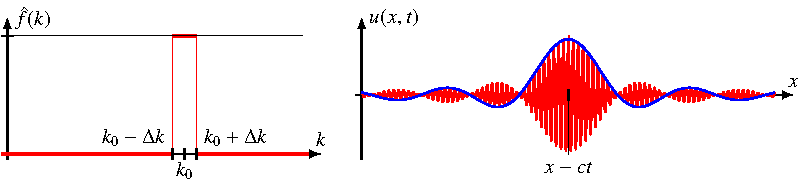
\includegraphics{chapters/7/wellenpaket.pdf}
\caption{Berechnung eines Wellenpaketes aus Wellen mit Wellenzahlen
zwischen $k_0-\Delta k$ und $k_0+\Delta k$.
\label{rossby:wellenpaket}}
\end{figure}
Wir betrachten ein Wellenpaket, welches als Überlagerung mit der
Amplitudenfunktion
\[
\hat f(k)
=
\begin{cases}
1&\qquad |k-k_0| < \Delta k\\
0&\qquad\text{sonst}
\end{cases}
\]
wie in Abbildung~\ref{rossby:wellenpaket} entsteht.
Die Überlagerung $u(x,t)$ gemäss~\eqref{rossby:komplexeueberlagerung}
kann man jetzt vereinfachen:
\[
u(x,t)
=
\operatorname{Re}
\int_{-\infty}^\infty \hat f(k)\,e^{i(kx-\omega(k)t)}\,dk
=
\operatorname{Re}
\int_{k_0-\Delta k}^{k_0+\Delta k} e^{i(kx-\omega(k)t)}\,dk,
\]
allerdings muss dazu $\omega(k)$ bekannt sein.

Falls $\omega(k)=ck$ gilt, falls also jede der elementaren Wellen
$\cos(kx-\omega t)$ die gleiche
Ausbreitungsgeschwindigkeit $c$ hat, können wir $u(x,t)$ explizit
ausrechnen:
\begin{align*}
u(x,t)
&=
\operatorname{Re}
\int_{k_0-\Delta k}^{k_0+\Delta k}
e^{i(kx-\omega(k)t)}\,dk
=
\operatorname{Re}
\int_{k_0-\Delta k}^{k_0+\Delta k}
e^{ik(x-ct)}\,dk
\\
&=
\operatorname{Re}
\biggl[
\frac{e^{ik(x-ct)}}{i(x-ct)}
\biggr]_{k_0-\Delta k}^{k_0+\Delta k}
=
\operatorname{Re}
\biggl(
\frac{e^{i(k_0+\Delta k)(x-ct)}}{i(x-ct)}
-
\frac{e^{i(k_0-\Delta k)(x-ct)}}{i(x-ct)}
\biggr)
\\
&=
\operatorname{Re}\frac{2}{x-ct}
e^{ik_0(x-ct)}\frac{e^{i\Delta k(x-ct)}-e^{i\Delta k(x-ct)}}{2i}
\\
&=
\operatorname{Re}\frac{2}{x-ct}
e^{ik_0(x-ct)}
\sin (\Delta k(x-ct))
=
2\cos k_0(x-ct) \frac{\sin \Delta k(x-ct)}{x-ct}
\end{align*}
Dies ist eine schnell schwankende Funktion mit Wellenzahl $k_0$, rot
dargestellt in Abbildung~\ref{rossby:wellenpaket} rechts, moduliert
mit der langsam schwankenden Funktion $\sin\Delta k(x-ct)/(x-ct)$,
dargestellt in der selben Abbildung in blau.
Der Schwerpunkt des Paketes befindet sich bei der $x$-Koordinaten $x-ct$,
er wandert also mit Geschwindigkeit $c$ nach rechts.

\subsubsection{Gruppengeschwindigkeit}
\index{Gruppengeschwindigkeit}%
Bisher haben wir angenommen, dass die Frequenz und die Wellenzahl proportional
sind, dass also $\omega(k)=ck$.
Die Untersuchungen zu den Rossby-Wellen hat gezeigt, dass dies nicht
zutreffen muss.
Wir müssen die Rechnung also mit einem Modell wiederholen, in dem die
Frequenz $\omega(k)$ nicht einfach nur proportional zu $k$ ist.
Für kleines $\Delta k$ genügt eine lineare Approximation der
Abhängigkeit von $\omega(k)$ von $k$, wir setzen daher
\begin{equation}
\omega(k)
=
\omega(k_0) + (k-k_0)\omega_1
=
\omega_0 + (k-k_0)\omega_1
\qquad
\text{mit}
\quad
\omega_1 = \frac{d}{dk}\omega(k_0) = \omega'(k_0).
\end{equation}
Wir berechnen wieder $u(x,t)$ wie folgt:
\begin{align*}
u(x,t)
&=
\operatorname{Re}
\int_{k_0-\Delta k}^{k_0+\Delta k}
e^{i(kx-\omega(k)t}\,dk
=
\operatorname{Re}
\int_{k_0-\Delta k}^{k_0+\Delta k}
e^{i(kx-\omega_0t -\omega_1(k-k_0)t)}
\,dk
\\
&=
\operatorname{Re}
\int_{k_0-\Delta k}^{k_0+\Delta k}
e^{i(k(x-\omega_1 t)-\omega_0t +\omega_1k_0t)}
\,dk
=
\operatorname{Re}
\int_{k_0-\Delta k}^{k_0+\Delta k}
e^{ik(x-\omega_1 t)}
e^{i(\omega_1k_0-\omega_0)t}
\,dk
\\
&=
\operatorname{Re}
e^{i(\omega_1k_0-\omega_0)t}
\biggl[
\frac{e^{ik(x-\omega_1 t)}}{i(x-\omega_1 t)}
\biggr]_{k_0-\Delta k}^{k_0+\Delta k}
=
\operatorname{Re}
2e^{i(\omega_1k_0-\omega_0)t}
\frac{
e^{i(k_0+\Delta k)(x-\omega_1 t)}
-
e^{i(k_0-\Delta k)(x-\omega_1 t)}
}{2i(x-\omega_1 t)}
\\
&=
\operatorname{Re}
\frac{2e^{i(\omega_1k_0-\omega_0)t}e^{i(k_0(x-\omega_1 t))}}{x-\omega_1 t}
\frac{
e^{i\Delta k(x-\omega_1 t)}
-
e^{-i\Delta k(x-\omega_1 t)}
}{2i}
=
\operatorname{Re}
2e^{i(\omega_1k_0-\omega_0+k_0(x-\omega_1 t))}
\frac{\sin \Delta k(x-\omega_1t)}{x-\omega_1 t}
\\
&=
\operatorname{Re}
2e^{i(k_0x-\omega_0t)}\,
\frac{\sin \Delta k(x-\omega_1t)}{x-\omega_1 t}
=
2\cos(k_0x-\omega_0t)
\frac{\sin \Delta k(x-\omega_1t)}{x-\omega_1 t}.
\end{align*}
Wiederum erhalten wir eine kurze Welle mit Frequenz
$\omega_0$ und Wellenzahl $k_0$, die moduliert wird mit der langsam
schwankenden Funktion
\begin{equation}
\frac{\sin\Delta k(x-\omega_1t)}{x-\omega_1 t}.
\label{rossby:gruppe}
\end{equation}
Das Maximum der Funktion~\eqref{rossby:gruppe}
befindet sich bei $x=\omega_1 t$, wandert also mit der
Geschwindigkeit $\omega_1$ nach rechts.

Die soeben durchgeführte Berechnung zeigt also, dass Wellenpakete
mit der Geschwindigkeit 
\[
c_g=\frac{d\omega(k)}{dk},
\]
der sogenannten {\em Gruppengeschwindigkeit}, wandern.
\index{Gruppengeschwindigkeit}%
Der Energietransport durch Wellenpakete erfolgt offenbar nicht
mit der Ausbreitungsgeschwindigkeit $c=\omega/k$, sondern mit der
Gruppengeschwindigkeit.

\subsection{Energietransport durch Rossby-Wellen\label{rossby:transport}}
Aus der Dispersionsrelation~\eqref{rossby:dispersion}
für die Rossby-Wellen können wir jetzt die Gruppengeschwindigkeit
für parallel zum Äquator sich bewegende Wellenpakete
durch Ableiten nach $k$ bestimmen.
Die Gruppengeschwindigkeit ist
\begin{equation}
c_g
=
\frac{d}{dk}\omega(k)
=
U-\beta
\frac{k^2+l^2-k\cdot 2k}{(k^2+l^2)^2}
=
U-\beta
\frac{l^2-k^2}{(k^2+l^2)^2}
\end{equation}
Je nach der relativen Grösse von $k$ und $l$ kann die
Gruppengeschwindigkeit sowohl grösser als auch kleiner sein als die
mittlere Geschwindigkeit $U$ in der Zone.
Rossby-Wellen können also je nach Wellenzahl sowohl nach Westen wie
auch nach Osten laufen.








%
% verzoegert.tex
%
% (c) 2018 Prof Dr Andreas Müller, Hochschule Rapperswil
%
\section{Verzögertes Oszillator-Modell\label{section:dde-nino}}
In den Kelvin- und Rossby-Wellen haben wir Mechanismen kennengelernt,
die Energietransport entlang des Äquators innerhalb der vorherrschenden
Strömung sowohl in östlicher wie auch in westlicher Richtung ermöglichen.
Entscheidend für die Dynamik dieses Energietransports ist die Zeit,
die eine Welle benötigt, um den Pazifik zu durchqueren.
Sei $\tau_K$ die Zeit, die eine Kelvin-Welle braucht, um den Pazifik
zu durchqueren, und $\tau_R$ die entsprechende Zeit für eine Rossby-Welle.

\rhead{Verzögertes Oszillator-Modell}
Wir versuchen jetzt, ein für die Temperaturanomalie $T(t)$ im östlichen
Pazifik aufzustellen, die diese Mechanismen berücksichtigt.
Ohne einen Transportmechanismus würde die Temperaturanomalie einfach
zerfallen, was beschrieben werden kann mit einer Differentialgleichung
der Form
\[
\frac{d}{dt}T(t)
=
-cT(t),
\]
mit einer Konstanten $c$.

\def\halb{\bgroup\textstyle\frac12\egroup}

Die Diskussionen über die dem El~Niño-Phänomen zugrunde liegenden
Mechanismen haben wir gesehen, dass die Thermoklinenanomalie im
zentralen Pazifik eine Auswirkung auf Temperatur\-anomalie $T(t)$ hat.
Eine Thermoklinenanomalie $h_0(t)$ am Äquator wandert als
Kelvin-Welle in der Zeit $\frac12\tau_K$ in den Ostpazifik.
Eine Thermoklinenanomalie $h_1(t)$ nördlich oder südlich des Äquators
kann als Rossby-Welle nach Westen wandern, am Westrand des Pazifik
reflektiert werden und als Kelvin-Welle in den Ostpazifik zurückkehren.
Dazu ist die Zeit $\frac12\tau_R+\tau_K$ nötig.
Dies lässt sich mit der Differentialgleichung
\begin{equation}
\frac{d}{dt}T(t)
=
-cT(t) + a_0h_0(t-\halb\tau_K) + b_0h_1(t-(\halb\tau_R+\tau_K))
\label{elninodde:1}
\end{equation}
erreichen.

Nun scheint es aber auch einen Zusammenhang zwischen der Temperaturanomalie
im Ostpazifik und den Thermoklinenanomalien im zentralen Pazifik zu geben.
Im einfachsten Fall kännen wir diesen Zusammenhang linear modellieren,
also 
\[
h_0(t-\halb\tau_K)
\sim
T(t-\halb\tau_K),
\qquad
\text{und}
\qquad
h_1(t-(\halb\tau_R+\tau_K))
\sim
T(t-(\halb\tau_R+\tau_K)).
\]
Eingesetzt in die Differentialgleichung~\eqref{elninodde:1} wird dabei zu
\begin{equation}
\frac{d}{dt}T(t)
=
-cT(t) + aT(t-\halb\tau_K) + bT(t-(\halb\tau_R+\tau_K))
\label{elninodde:2}
\end{equation}
Die Ableitung $\dot T(t)$ hängt also nicht nur von der Temperaturanomalie
zur Zeit $t$ ab, sondern auch von den Temperaturanomalien zu den
früheren Zeitpunkten $t-\halb\tau_K$ und $t-(\halb\tau_R-\tau_K)$.
Man nennt
\eqref{elninodde:2}
eine verzögerte Differentialgleichung.
\index{verzögerte Differentialgleichung}%

Die Theorie der linearen, verzögerten Differentialgleichungen wie 
\eqref{elninodde:2} zeigt, dass sie ähnlich wie gewöhnliche linear
Differentialgleichungen erster Ordnung Lösungen haben, die exponentiell
schnell zerfallen oder exponentiell anwachsen.
Daher können wir nicht erwarten, dass \eqref{elninodde:2} das El~Niño-Phänomen
adäquat beschreiben kann.
Um das exponentielle Anwachsen zu verhindern, braucht es einen zusätzlichen
Term, der dem Anwachsen von $T(t)$ überproportional entgegenwirkt.
Zum Beispiel könnte dies man mit einem Term der Form $-\varepsilon T(t)^3$
erreichen.
Die verzögerte Differentialgleichung ist dann
\begin{equation}
\frac{d}{dt}T(t)
=
-cT(t) + aT(t-\halb\tau_K) + bT(t-(\halb\tau_R+\tau_K))
-\varepsilon T(t)^3.
\label{elninodde:3}
\end{equation}
Ein andere Möglichkeit, ein ähnliches Ziel zu erreichen, wird in Kapitel
\ref{chapter:planeten} dargestellt.

In Kapitel~\ref{chapter:verzoegert} wird das Verhalten der Lösungen
solcher verzögerter Differentialgleichungen etwas mehr im Detail
diskutiert und es wird gezeigt, dass sie tatsächlich wesentliche
Aspekte des El~Niño-Phänomens adäquat wiedergeben können.










%
% assim.tex
%
% (c) 2018 Prof Dr Andreas Müller, Hochschule Rapperswil
%
\chapter{Datenassimilation}


\begin{appendices}
%\input{chapters/konstanten.tex}
%\input{chapters/komplexezahlen.tex}
\end{appendices}
\vfill
\pagebreak
\ifodd\value{page}\else\null\clearpage\fi
\lhead{Literatur}
\rhead{}
\printbibliography[heading=subbibliography]
\label{skript:literatur}
\end{refsection}

\part{Anwendungen und Weiterführende Themen}
\lhead{Anwendungen}
%
% uebersicht.tex -- Uebersicht ueber die Seminar-Arbeiten
%
% (c) 2018 Prof Dr Andreas Mueller, Hochschule Rapperswil
%
\chapter*{"Ubersicht}
\lhead{"Ubersicht}
\rhead{}
\label{skript:uebersicht}
Im zweiten Teil kommen die Teilnehmer des Seminars selbst zu Wort.
Die im ersten Teil dargelegten mathematischen Methoden und
grundlegenden Modelle werden dabei verfeinert, verallgemeinert
und auch numerisch überprüft.
Die Beispiele zeigen auch, dass umfassende Klimamodell erwartungsgemäss
schnell sehr komplex werden können.
Sie zeigen aber auch, dass es möglich ist, wesentliche Aspekte
des Klimas aus einfachen Überlegungen und mit übersichtlichen
mathematischen Modellen zu erfassen und zu verstehen.

{\em Matthias Baumann} und {\em Oliver Dias} zeigen zusätzliche
Informationen zum Lorenz-System, insbesondere zum Lorenz-Attraktor.
{\em Hansruedi Patzen} verallgemeinert das Vorgehen, mit dem das
Lorenz-System gewonnen wurde, im Sinne des Separationsverfahrens
für partielle Differentialgleichungen weiter, und gewinnt eine
Reihe von höherdimensionalen Lorenz-Systemen und untersucht weiter,
ob das beim dreidimensionalen System gefundene chaotische Verhalten 
auch in den höherdimensionalen Versionen zu finden ist.
Diese Untersuchungen zeigen, dass das Verhalten wahrscheinlich
nicht nur ein Artefakt der Reduktion auf drei Dimensionen ist, sondern
eine inhärente Eigenschaft des Lorenz-Systems.

Die exakte Lösung von Klimamodellen ist oft sehr schwierig, oft sind
Parameter oder Abhängigkeiten nicht bekannt.
Ein alternativer Ansatz ist daher, die zeitliche Entwicklung
im Sinne von machine learning zu lernen.
{\em Martin Stypinski} untersucht diesen Ansatz an zwei Beispielen,
der Wärmeleitungsgleichung und der nichtlinearen Gleichung von Burgers.
Die Beispiele zeigen vor allem auch, wie mathematisches Wissen über das
Modell hilft, die neuronalen Netzwerke zweckmässig zu entwerfen.

Die im Text entwickelten Modelle sind meist noch rudimentär, eine
reihe von Arbeiten haben sich daher mit Erweiterungen und Verfeinerungen
befasst.
{\em Jonas Gründler} hat das 2-Box Modell der thermohalinen Zirkulation
auf 3 Boxen verallgemeinert.
{\em Silvio Marti} studiert den Einfluss von Eis auf das Klima.
Die verzögerte Differentialgleichung des El Niño-Systems kann
numerische gelöst werden. {\em Raphael Unterer} zeigt, wie dies
funktioniert und findet insbesondere auch eine Stabilitätsbedingung
für sein Verfahren.
{\em Nicolas Tobler} hat versucht, die Modelle auf verschiedene
Planeten zu verallgemeinern und damit die Unterschiede der Atmosphären
der Planeten Venus, Erde und Mars zu erklären.
Die Einflüsse anderer Planeten zeigen sich zum Beispiel in der
Neigung der Erdachse gegen die Erdbahnebene.
Wie {\em Sebastian Lenhard} vorführt, können auch kleine Änderungen
der Neigung das Klima dramatisch verändern.
%Schliesslich gibt es auch eine Kopplung zwischen Klima und
%Vegetation, die {\em Matthias Dunkel} modelliert hat.

Die letzten zwei Kapitel befassen sich mit der Aufarbeitung der
Daten, auf grund derer wir zum Schluss kommen, dass 
der Klimawandel real ist.
Für Wetter- wie auch für Klimamodelle sind grosse Datenmengen
von Wetter- und Klimamessstationen in die Rechnung zu integrieren.
Der Kalman-Filter ist die Basis vieler moderner Lösungsansätze
für dieses Problem.
Am Beispiel des erweiterten Kalman-Filters für das Lorenz-System
zeigt {\em Michael Müller}, wie es möglich ist, den Systemzustand
selbst eines chaotischen nichtlinearen Systems zu 
Extreme Ereignisse sind in den letzten Jahren häufiger geworden
und werden oft als Indikatoren für die Klimaveränderung angeführt.
Wie man mit statistischen Daten über solche Ereignisse beweisen
kann, dass der Klimawandel tatsächlich stattfindet, zeigt
{\em Melina Staub}.






\def\chapterauthor#1{{\large #1}\bigskip\bigskip}
% Artikeverzoegert
%
% main.tex -- Paper zum Thema <thema>
%
% (c) 2018 Hochschule Rapperswil
%
\chapter{Achsneigung und Eiszeiten\label{chapter:thema}}
\lhead{Achseneigung und Eiszeiten}
\begin{refsection}
\chapterauthor{Sebastian Lenhard}

\section{Abschnitt}
\rhead{Abschnitt}

\section{Schlussfolgerung}
\rhead{Schlussfolgerung}

\printbibliography[heading=subbibliography]
\end{refsection}

%
% main.tex -- Paper zum Thema <thema>
%
% (c) 2018 Hochschule Rapperswil
%
\chapter{Achsneigung und Eiszeiten\label{chapter:thema}}
\lhead{Achseneigung und Eiszeiten}
\begin{refsection}
\chapterauthor{Sebastian Lenhard}

\section{Abschnitt}
\rhead{Abschnitt}

\section{Schlussfolgerung}
\rhead{Schlussfolgerung}

\printbibliography[heading=subbibliography]
\end{refsection}

%
% main.tex -- Paper zum Thema <thema>
%
% (c) 2018 Hochschule Rapperswil
%
\chapter{Achsneigung und Eiszeiten\label{chapter:thema}}
\lhead{Achseneigung und Eiszeiten}
\begin{refsection}
\chapterauthor{Sebastian Lenhard}

\section{Abschnitt}
\rhead{Abschnitt}

\section{Schlussfolgerung}
\rhead{Schlussfolgerung}

\printbibliography[heading=subbibliography]
\end{refsection}

%
% main.tex -- Paper zum Thema <thema>
%
% (c) 2018 Hochschule Rapperswil
%
\chapter{Achsneigung und Eiszeiten\label{chapter:thema}}
\lhead{Achseneigung und Eiszeiten}
\begin{refsection}
\chapterauthor{Sebastian Lenhard}

\section{Abschnitt}
\rhead{Abschnitt}

\section{Schlussfolgerung}
\rhead{Schlussfolgerung}

\printbibliography[heading=subbibliography]
\end{refsection}

%
% main.tex -- Paper zum Thema <thema>
%
% (c) 2018 Hochschule Rapperswil
%
\chapter{Achsneigung und Eiszeiten\label{chapter:thema}}
\lhead{Achseneigung und Eiszeiten}
\begin{refsection}
\chapterauthor{Sebastian Lenhard}

\section{Abschnitt}
\rhead{Abschnitt}

\section{Schlussfolgerung}
\rhead{Schlussfolgerung}

\printbibliography[heading=subbibliography]
\end{refsection}

%
% main.tex -- Paper zum Thema <thema>
%
% (c) 2018 Hochschule Rapperswil
%
\chapter{Achsneigung und Eiszeiten\label{chapter:thema}}
\lhead{Achseneigung und Eiszeiten}
\begin{refsection}
\chapterauthor{Sebastian Lenhard}

\section{Abschnitt}
\rhead{Abschnitt}

\section{Schlussfolgerung}
\rhead{Schlussfolgerung}

\printbibliography[heading=subbibliography]
\end{refsection}

%
% main.tex -- Paper zum Thema <thema>
%
% (c) 2018 Hochschule Rapperswil
%
\chapter{Achsneigung und Eiszeiten\label{chapter:thema}}
\lhead{Achseneigung und Eiszeiten}
\begin{refsection}
\chapterauthor{Sebastian Lenhard}

\section{Abschnitt}
\rhead{Abschnitt}

\section{Schlussfolgerung}
\rhead{Schlussfolgerung}

\printbibliography[heading=subbibliography]
\end{refsection}

%
% main.tex -- Paper zum Thema <thema>
%
% (c) 2018 Hochschule Rapperswil
%
\chapter{Achsneigung und Eiszeiten\label{chapter:thema}}
\lhead{Achseneigung und Eiszeiten}
\begin{refsection}
\chapterauthor{Sebastian Lenhard}

\section{Abschnitt}
\rhead{Abschnitt}

\section{Schlussfolgerung}
\rhead{Schlussfolgerung}

\printbibliography[heading=subbibliography]
\end{refsection}

%
% main.tex -- Paper zum Thema <thema>
%
% (c) 2018 Hochschule Rapperswil
%
\chapter{Achsneigung und Eiszeiten\label{chapter:thema}}
\lhead{Achseneigung und Eiszeiten}
\begin{refsection}
\chapterauthor{Sebastian Lenhard}

\section{Abschnitt}
\rhead{Abschnitt}

\section{Schlussfolgerung}
\rhead{Schlussfolgerung}

\printbibliography[heading=subbibliography]
\end{refsection}

%
% main.tex -- Paper zum Thema <thema>
%
% (c) 2018 Hochschule Rapperswil
%
\chapter{Achsneigung und Eiszeiten\label{chapter:thema}}
\lhead{Achseneigung und Eiszeiten}
\begin{refsection}
\chapterauthor{Sebastian Lenhard}

\section{Abschnitt}
\rhead{Abschnitt}

\section{Schlussfolgerung}
\rhead{Schlussfolgerung}

\printbibliography[heading=subbibliography]
\end{refsection}

%
% main.tex -- Paper zum Thema <thema>
%
% (c) 2018 Hochschule Rapperswil
%
\chapter{Achsneigung und Eiszeiten\label{chapter:thema}}
\lhead{Achseneigung und Eiszeiten}
\begin{refsection}
\chapterauthor{Sebastian Lenhard}

\section{Abschnitt}
\rhead{Abschnitt}

\section{Schlussfolgerung}
\rhead{Schlussfolgerung}

\printbibliography[heading=subbibliography]
\end{refsection}

\vfill
\pagebreak
\ifodd\value{page}\else\null\clearpage\fi
\lhead{Index}
\rhead{}
\addcontentsline{toc}{chapter}{\indexname}
%
% skript.tex -- Skript ueber Klimawandel
%
% (c) 2017 Prof. Dr. Andreas Mueller, HSR
%
\documentclass{book}
\usepackage{etex}
\usepackage{geometry}
\geometry{papersize={170mm,240mm},total={140mm,200mm},top=21mm,bindingoffset=10mm}
\usepackage[english,ngerman]{babel}
\usepackage[utf8]{inputenc}
\usepackage[T1]{fontenc}
\usepackage{cancel}
\usepackage{times}
\usepackage{amsmath,amscd}
\usepackage{amssymb}
\usepackage{amsfonts}
\usepackage{amsthm}
\usepackage{graphicx}
\usepackage{fancyhdr}
\usepackage{textcomp}
\usepackage{txfonts}
%\usepackage{alltt} 
\newcommand\hmmax{0}
\newcommand\bmmax{0}
\usepackage{bm}
\usepackage{verbatim}
\usepackage{paralist}
\usepackage{makeidx}
\usepackage{array}
%\usepackage[colorlinks=true]{hyperref}
\usepackage{hyperref}
\usepackage{tikz}
\usepackage{pgfplots}
\usepackage{pgfplotstable}
\usepackage{pdftexcmds}
\usepackage{pgfmath}
%\usepackage{placeins}
%\usepackage{subfigure}
\usepackage[autostyle=false,english=american]{csquotes}
%\usepackage{float}
%\usepackage{enumitem}
\usepackage{wasysym}
\usepackage{environ}
%\usepackage{pifont}
%\usepackage{feynmp}
\usepackage{appendix}
\usetikzlibrary{calc,intersections,through,backgrounds,graphs,positioning,shapes,arrows,fit}
\usetikzlibrary{patterns,decorations.pathreplacing}
\usetikzlibrary{decorations.pathreplacing}
\usetikzlibrary{external}
\usetikzlibrary{datavisualization}
\usepackage[europeanvoltages,
            europeancurrents,
            europeanresistors,   % rectangular shape
            americaninductors,   % "4-bumbs" shape
            europeanports,       % rectangular logic ports
            siunitx,             % #1<#2>
            emptydiodes,
            noarrowmos,
            smartlabels]         % lables are rotated in a smart way
           {circuitikz}          %
\usepackage{siunitx}
\usepackage{tabularx}
\usetikzlibrary{arrows}

\usepackage{algpseudocode}
\usepackage{algorithm}
\usepackage{gensymb}
\usepackage{mathtools}


% Matlab
\usepackage{listings}
\usepackage{color} %red, green, blue, yellow, cyan, magenta, black, white
\definecolor{mygreen}{RGB}{28,172,0} % color values Red, Green, Blue
\definecolor{mylilas}{RGB}{170,55,241}

\lstset{language=Matlab,%
    %basicstyle=\color{red},
    breaklines=true,%
    morekeywords={matlab2tikz},
    keywordstyle=\color{blue},%
    morekeywords=[2]{1}, keywordstyle=[2]{\color{black}},
    identifierstyle=\color{black},%
    stringstyle=\color{mylilas},
    commentstyle=\color{mygreen},%
    showstringspaces=false,%without this there will be a symbol in the places where there is a space
    numbers=left,%
    %numberstyle={\tiny \color{black}},% size of the numbers
    numbersep=9pt, % this defines how far the numbers are from the text
    emph=[1]{break},emphstyle=[1]\color{red}, %some words to emphasise
    %emph=[2]{word1,word2}, emphstyle=[2]{style},    
}
\lstdefinestyle{Matlab}{
  numbers=left,
  belowcaptionskip=1\baselineskip,
  breaklines=true,
  frame=L,
  xleftmargin=\parindent,
  language=Matlab,
  showstringspaces=false,
  basicstyle=\footnotesize\ttfamily,
  keywordstyle=\bfseries\color{green!40!black},
  commentstyle=\itshape\color{purple!40!black},
  identifierstyle=\color{blue},
  stringstyle=\color{orange},
  numberstyle=\ttfamily\tiny
}
\lstdefinelanguage{Matlab}{
  keywords={function,global,size,zeros,switch,case,otherwise,end,sin,cos,cot,floor,ode45,hold,polarplot},
  sensitive=true
}
\lstdefinelanguage{Maxima}{
  keywords={addrow,addcol,zeromatrix,ident,augcoefmatrix,ratsubst,sum,diff,ev,tex,%
    with_stdout,nouns,express,depends,load,length,submatrix,div,grad,curl,matrix,%
    invert,lambda,facsum,expand,false,then,if,else,subst,batchload,%
    rootscontract,solve,part,assume,sqrt,integrate,abs,inf,exp,sin,cos,sinh,cosh,taylor,ratsimp},
  sensitive=true,
  comment=[n][\itshape]{/*}{*/}
}
\lstdefinestyle{Maxima}{
  numbers=left,
  belowcaptionskip=1\baselineskip,
  breaklines=true,
  frame=L,
  xleftmargin=\parindent,
  language=Maxima,
  showstringspaces=false,
  basicstyle=\footnotesize\ttfamily,
  keywordstyle=\bfseries\color{green!40!black},
  commentstyle=\itshape\color{purple!40!black},
  identifierstyle=\color{blue},
  stringstyle=\color{orange},
  numberstyle=\ttfamily\tiny
}
\lstset{language=Octave,%
    %basicstyle=\color{red},
    breaklines=true,%
    morekeywords={function,global,size,zeros,switch,case,otherwise,end,sin,cos,cot,floor,ode45,hold,polarplot,endfunction,size,endswitch,cat,printf,for,endfor,if,return,endif,abs,while,endwhile},
    keywordstyle=\color{blue},%
    morekeywords=[2]{1}, keywordstyle=[2]{\color{black}},
    identifierstyle=\color{black},%
    stringstyle=\color{mylilas},
    commentstyle=\color{mygreen},%
    showstringspaces=false,%without this there will be a symbol in the places where there is a space
    numbers=left,%
    %numberstyle={\tiny \color{black}},% size of the numbers
    numbersep=9pt, % this defines how far the numbers are from the text
    emph=[1]{break},emphstyle=[1]\color{red}, %some words to emphasise
    %emph=[2]{word1,word2}, emphstyle=[2]{style},    
}
\lstdefinestyle{Octave}{
  numbers=left,
  belowcaptionskip=1\baselineskip,
  breaklines=true,
  frame=L,
  xleftmargin=\parindent,
  language=Octave,
  showstringspaces=false,
  basicstyle=\footnotesize\ttfamily,
  keywordstyle=\bfseries\color{green!40!black},
  commentstyle=\itshape\color{purple!40!black},
  identifierstyle=\color{blue},
  stringstyle=\color{orange},
  numberstyle=\ttfamily\tiny
}
\lstdefinestyle{C}{
  numbers=left,
  belowcaptionskip=1\baselineskip,
  breaklines=true,
  frame=L,
  xleftmargin=\parindent,
  language=C,
  showstringspaces=false,
  basicstyle=\footnotesize\ttfamily,
  keywordstyle=\bfseries\color{green!40!black},
  commentstyle=\itshape\color{purple!40!black},
  identifierstyle=\color{blue},
  stringstyle=\color{orange},
  numberstyle=\ttfamily\tiny
}
\usepackage{caption}
\usepackage[mode=buildnew]{standalone}
\usepackage[backend=bibtex]{biblatex}

% additional packages
%
% packages.tex -- zusätzliche Packages 
%
% In diesem File werden \usepackage{}-Aufrufe eingetragen für Packages, die
% noch nicht im skript.tex aufgerufen werden
%
% (c) 2018 Michael Müller, Hochschule Rapperswil
%


%
% packages.tex -- zusätzliche Packages 
%
% In diesem File werden \usepackage{}-Aufrufe eingetragen für Packages, die
% noch nicht im skript.tex aufgerufen werden
%
% (c) 2018 Michael Müller, Hochschule Rapperswil
%


%
% packages.tex -- zusätzliche Packages 
%
% In diesem File werden \usepackage{}-Aufrufe eingetragen für Packages, die
% noch nicht im skript.tex aufgerufen werden
%
% (c) 2018 Michael Müller, Hochschule Rapperswil
%


%
% packages.tex -- zusätzliche Packages 
%
% In diesem File werden \usepackage{}-Aufrufe eingetragen für Packages, die
% noch nicht im skript.tex aufgerufen werden
%
% (c) 2018 Michael Müller, Hochschule Rapperswil
%


%
% packages.tex -- zusätzliche Packages 
%
% In diesem File werden \usepackage{}-Aufrufe eingetragen für Packages, die
% noch nicht im skript.tex aufgerufen werden
%
% (c) 2018 Michael Müller, Hochschule Rapperswil
%


%
% packages.tex -- zusätzliche Packages 
%
% In diesem File werden \usepackage{}-Aufrufe eingetragen für Packages, die
% noch nicht im skript.tex aufgerufen werden
%
% (c) 2018 Michael Müller, Hochschule Rapperswil
%


%
% packages.tex -- zusätzliche Packages 
%
% In diesem File werden \usepackage{}-Aufrufe eingetragen für Packages, die
% noch nicht im skript.tex aufgerufen werden
%
% (c) 2018 Michael Müller, Hochschule Rapperswil
%


%
% packages.tex -- zusätzliche Packages 
%
% In diesem File werden \usepackage{}-Aufrufe eingetragen für Packages, die
% noch nicht im skript.tex aufgerufen werden
%
% (c) 2018 Michael Müller, Hochschule Rapperswil
%


%
% packages.tex -- zusätzliche Packages 
%
% In diesem File werden \usepackage{}-Aufrufe eingetragen für Packages, die
% noch nicht im skript.tex aufgerufen werden
%
% (c) 2018 Michael Müller, Hochschule Rapperswil
%


%
% packages.tex -- zusätzliche Packages 
%
% In diesem File werden \usepackage{}-Aufrufe eingetragen für Packages, die
% noch nicht im skript.tex aufgerufen werden
%
% (c) 2018 Michael Müller, Hochschule Rapperswil
%



% workaround for biblatex bug
\makeatletter
\def\blx@maxline{77}
\makeatother
\addbibresource{references.bib}
% Bibresources für jeden einzelnen Artikel
%\addbibresource{eis/references.bib}
%\addbibresource{extrem/references.bib}
%\addbibresource{kalman/references.bib}
%\addbibresource{learning/references.bib}
\addbibresource{lorenz/references.bib}
%\addbibresource{lorenz2/references.bib}
%\addbibresource{planeten/references.bib}
%\addbibresource{thermohalin/references.bib}
%\addbibresource{vegetation/references.bib}
%\addbibresource{verzoegert/references.bib}
\AtEndDocument{\clearpage\ifodd\value{page}\else\null\clearpage\fi}
\makeindex
%\pgfplotsset{compat=1.12}
\setlength{\headheight}{15pt} % fix headheight warning
\DeclareGraphicsRule{*}{mps}{*}{}
\begin{document}
\pagestyle{fancy}
\frontmatter
\newcommand\HRule{\noindent\rule{\linewidth}{1.5pt}}
\begin{titlepage}
\vspace*{\stretch{1}}
\HRule
\vspace*{5pt}
\begin{flushright}
{
\LARGE
Mathematisches Seminar\\
\vspace*{20pt}
\Huge
Klimawandel%
}
\vspace*{5pt}
\end{flushright}
\HRule
\begin{flushright}
\vspace{60pt}
\Large
Leitung: Andreas M"uller\\
\vspace{40pt}
\Large
%
% teilnehmer.tex -- Liste der Seminarteilnehmer für Titelseite
%
% (c) 2018 Prof Dr Andreas Müller, Hochschule Rapperswil
%
Matthias Baumann,
Oliver Dias-Lalcaca,
%Matthias Dunkel%,
Jonas Gründler%,
\\
Sebastian Lenhard,
Silvio Marti,
Michael~Müller,
Hansruedi~Patzen%,
\\
Melina~Staub,
Martin~Stypinski,
Nicolas Tobler,
Raphael Unterer
\\

%Matthias Baumann,
%Oliver Dias-Lalcaca,
%Matthias Dunkel%,
%\\
%Flurina Hoby,
%Sebastian Lenhard,
%Silvio Marti,
%Hansruedi~Patzen%,
%\\
%Melina~Staub,
%Martin~Stypinski,
%Nicolas Tobler,
%Raphael Unterer
\end{flushright}
\vspace*{\stretch{2}}
\begin{center}
Hochschule f"ur Technik, Rapperswil, 2018
\end{center}
\end{titlepage}
\hypersetup{
    linktoc=all,
    linkcolor=blue
}
\newcounter{beispiel}
\newenvironment{beispiele}{
\bgroup\smallskip\parindent0pt\bf Beispiele\egroup

\begin{list}{\arabic{beispiel}.}
  {\usecounter{beispiel}
  \setlength{\labelsep}{5mm}
  \setlength{\rightmargin}{0pt}
}}{\end{list}}
\newcounter{uebungsaufgabezaehler}
% environment fuer uebungsaufgaben
\newenvironment{uebungsaufgaben}{
\begin{list}{\arabic{uebungsaufgabezaehler}.}
  {\usecounter{uebungsaufgabezaehler}
  \setlength{\labelwidth}{2cm}
  \setlength{\leftmargin}{0pt}
  \setlength{\labelsep}{5mm}
  \setlength{\rightmargin}{0pt}
  \setlength{\itemindent}{0pt}
}}{\end{list}\vfill\pagebreak}
\newenvironment{teilaufgaben}{
\begin{enumerate}
\renewcommand{\labelenumi}{\alph{enumi})}
}{\end{enumerate}}
% Aufgabe
\newcounter{problemcounter}[chapter]
\def\aufgabenpath{chapters/uebungsaufgaben/}
\def\ainput#1{\input\aufgabenpath/#1}
\def\verbatimainput#1{\expandafter\verbatiminput{\aufgabenpath/#1}}
\def\aufgabetoplevel#1{%
\expandafter\def\expandafter\inputpath{#1}%
\let\aufgabepath=\inputpath
}
\def\includeagraphics[#1]#2{\expandafter\includegraphics[#1]{\aufgabepath#2}}
% \aufgabe
\newcommand{\uebungsaufgabe}[1]{%
\refstepcounter{problemcounter}%
\label{#1}%
\bigskip{\parindent0pt\strut}\hbox{\bf\arabic{problemcounter}. }%
\expandafter\def\csname aufgabenpath\endcsname{\inputpath/}%
\expandafter\input{chapters/uebungsaufgaben/#1.tex}
}
\renewcommand\theproblemcounter{\thechapter.\arabic{problemcounter}}

% Loesung
\def\swallow#1{
%nothing
}
\NewEnviron{loesung}[1][L"osung]{%
\begin{proof}[#1]%
\renewcommand{\qedsymbol}{$\bigcirc$}
\BODY
\end{proof}
}
\NewEnviron{bewertung}{%
\begin{proof}[Bewertung]%
\renewcommand{\qedsymbol}{}
\BODY
\end{proof}
}
\NewEnviron{diskussion}{%
\begin{proof}[Diskussion]%
\renewcommand{\qedsymbol}{}
\BODY
\end{proof}
}
\NewEnviron{hinweis}{%
\begin{proof}[Hinweis]%
\renewcommand{\qedsymbol}{}
\BODY
\end{proof}
}
\def\keineloesungen{%
\RenewEnviron{loesung}{\relax}
\RenewEnviron{bewertung}{\relax}
\RenewEnviron{diskussion}{\relax}
}
\newenvironment{beispiel}{%
\begin{proof}[Beispiel]%
\renewcommand{\qedsymbol}{$\bigcirc$}
}{\end{proof}}

\allowdisplaybreaks

\lhead{Inhaltsverzeichnis}
\rhead{}
\tableofcontents
\newtheorem{satz}{Satz}[chapter]
\newtheorem{hilfssatz}[satz]{Hilfssatz}
\newtheorem{definition}[satz]{Definition}
\newtheorem{annahme}[satz]{Annahme}
\newtheorem{problem}[satz]{Problem}
\newtheorem*{problem*}{Problem}
\renewcommand{\floatpagefraction}{0.7}
\mainmatter
%
% vorwort.tex -- Vorwort zum Buch zum Seminar
%
% (c) 2017 Prof Dr Andreas Mueller, Hochschule Rapperswil
%
\chapter*{Vorwort}
\lhead{Vorwort}
\rhead{}
Dieses Buch entstand im Rahmen des Mathematischen Seminars
im Frühjahrssemester 2017 an der Hochschule für Technik Rapperswil.
Die Teilnehmer, Studierende der Abteilungen für Elektrotechnik,
Informatik und Bauingenieurwesen der
HSR, erarbeiteten nach einer Einführung in das Themengebiet jeweils
einzelne Aspekte des Gebietes in Form einer Seminararbeit, über
deren Resultate sie auch in einem Vortrag informierten. 

Im Frühjahr 2018 war das Thema des Seminars der Klimawandel.

Im zweiten Teil dieses Skripts kommen dann die Teilnehmer selbst zu Wort.
Ihre Arbeiten wurden jeweils als einzelne
Kapitel mit meist nur typographischen Änderungen übernommen.
Diese weiterführenden Kapitel sind sehr verschiedenartig.
Eine Übersicht und Einführung findet sich in der Einleitung
zum zweiten Teil auf Seite~\pageref{skript:uebersicht}.

In einigen Arbeiten wurde auch Code zur Demonstration der 
besprochenen Methoden und Resultate geschrieben, soweit
möglich und sinnvoll wurde dieser Code im Github-Repository
dieses Kurses%
\footnote{\url{https://github.com/AndreasFMueller/SeminarKlima.git}}
abgelegt.

Im genannten Repository findet sich auch der Source-Code dieses
Skriptes, es wird hier unter einer Creative Commons Lizenz
zur Verfügung gestellt.
Auf der beiliegenden DVD befinden sich die Testdaten und Programme
zu zwei der simulationsintensiveren Artikel im zweiten Teil.



\part{Grundlagen}
%\keineloesungen
\begin{refsection}
%
% part1.tex
%
% (c) 2018 Prof Dr Andreas Müller, Hochschule Rapperswil
%
%
% wuk.tex -- Wetter und Klima
%
% Einleitungskapitel, welches das Wetter- und Klimasystem der Erde in
% qualitiativer Form beschreibt
%
% (c) 2018 Prof Dr Andreas Müller, Hochschule Rapperswil
%
\chapter{Wetter und Klima\label{chapter:wetter und klima}}
\lhead{Wetter und Klima}
US Präsident Donald Trump war schon immer ein Klimaverweigerer, wie Tweets
aus der Zeit lange bevor er Präsident wurde:
\begin{center}

\includegraphics[width=\hsize]{chapters/1/trump.png}
\end{center}
Ganz offensichtlich versteht Trump den Unterschied zwischen Wetter und
Klima nicht.
Ziel dieses Kapitels ist, den Unterschied zwischen Wetter und Klima
zu klären.
Es ist allgemein bekannt, dass auch die besten Wetterprognosen im
günstigsten Fall für einige Tage zutreffen.
Daher soll in diesem Kapitel auch gezeigt werden, warm trotz dieser
Schwierigkeit das Klima sehr wohl langfristig modelliert und prognostiziert
werden kann.
Aus diesen Überlegungen wird auch klar, auf welche Aspekte des Klimasystems
sich ein Klima-Modell fokusieren muss, wenn eine langfristige Prognose
ermöglicht werden soll.

\input{chapters/1/klima.tex}
\input{chapters/1/physik.tex}
\input{chapters/1/anforderungen.tex}

%\section{Klima}
%\rhead{Klima}
%In der Wikipedia kann man die folgenden Definitionen für die Begriffe Wetter
%und Klima finden:
%
%\begin{definition}
%Als {\em Wetter} bezeichnet man den
%spürbaren, kurzfristigen Zustand der Atmosphäre (auch: messbarer
%Zustand der Troposphäre) an einem bestimmten Ort der Erdoberfläche,
%der unter anderem als Sonnenschein, Bewölkung, Regen, Wind, Hitze
%oder Kälte in Erscheinung tritt.
%\cite{skript:wetter}
%\end{definition}
%
%\begin{definition}
%Das {\em Klima} steht als Begriff für die Gesamtheit aller meteorologischen
%Vorgänge, die für die über Zeiträume von mindestens 30 Jahren
%regelmässig wiederkehrenden durchschnittlichen Zustände der Erdatmosphäre
%an einem Ort verantwortlich sind.
%\cite{skript:klima}
%\end{definition}
%
%Was also Donald Trump in seinem Tweet beschrieben hat ist das Wetter.
%Selbst wenn die Temperatur in New York unter den Gefrierpunkt fällt, 
%heisst das nicht, dass die mittlere Temperatur in New York über mehrere
%Jahre nicht doch ansteigen kann.
%Tatsächlich bedeutet ``globale Erwärmung'' nicht, dass die mittlere
%Temperatur an jedem Punkt der Erde zunehmen wird.
%Im Gegenteil ist es durchaus möglich, dass zwar die mittlere Temperatur
%der Erde ständig zunimmt, wie wir in den letzten Jahren auch messtechnisch
%nachweisen konnten, dass aber auch die Temperaturunterschiede stark zunehmen,
%so dass es am Ende an einzelnen Stelle der Erdoberfläche zu einer 
%Abkühlung kommen kann.
%Um dieser Komplexität Rechnung zu tragen, spricht man nicht mehr von
%der ``globalen Erwärmung'', sondern vom Klimawandel.
%
%Auch wenn das Wetter nur sehr eingeschränkt vorhersagen lässt,
%bedeutet das noch lange nicht, dass das Klima nicht doch sehr
%genau vorhergesagt werden kann.
%Eine Analogie kann den Unterschied zwischen der Vorhersagbarkeit
%von Wetter und Klima verdeutlichen.
%Wenn man in einem Kochtopf Wasser zum Kochen bringt, stellt sich
%eine unverrhersagbare chaotische Bewegung kleiner und grosser
%Gasblasen ein.
%Es ist unmöglich vorherzusagen, wann und wo sich die nächste Blase
%bilden wird und welchen Weg sie an die Oberfläche des Wasser nehmen
%wird.
%Wenn wir aber nur die mittlere Temperatur betrachten, können wir
%aus der Heizleistung der Kochplatte, der Masse und der spezifischen
%Wärmekapazität des Wassers genau berechnen, welche Temperatur zu welcher
%Zeit im Wasser herschen wird und wir können den Zeitpunkt exakt
%vorhersagen, wann das Wasser zu sieden beginnt.
%Die mittlere Temperatur des Wassers beschreibt das ``Klima''
%in der Pfanne, die kleinräumigen und kurzfristigen Blasen und anderen
%Turbulenzen beschreiben das ``Wetter''.
%
%\section{Physikalische Eigenschaften des Klimasystems}
%In diesem Abschnitt stellen wir die physikalischen Eigenschaften
%aller wesentlicher Komponenten des Klimasystems zusammen.
%Dabei geht es zunächst nur darum, die grundlegende Physik in 
%Erinnerung zu rufen und die Naturgesetze, die die Wechselwirkungen
%zwischen den Komponenten beschreiben.
%Auf die Details der mathematischen Modellierung der zukünftigen
%Veränderung dieser Grössen werden wir erst später eingehen.
%
%\subsection{Wärme, Konvektion, Kondensation}
%Die wohl wichtigste Klima-Grösse ist die Temperatur.
%Sie drückt aus, wieviel Energie in Form von Wärme ein Körper enthält.
%
%\subsubsection{Wärmekapazität}
%Die spezifische Wärme $C$ gibt an, wie die innere Energie sich bei
%einer Temperaturänderung $\Delta T$ verändert:
%\[
%\Delta E = C\cdot\Delta T.
%\]
%Der Körper speichert Energie in Form der thermischen Bewegung der
%einzelnen Atome.
%Schwerere Atome können bei gleicher Bewegungsgeschwindigkeit 
%mehr Energie speichern.
%Stoffe mit grösserer Dichte können mehr Atome und damit auch mehr
%Wärmeenergie in einem kleineren Volumen unterbringen.
%Die spezifische Wärmekapazität $c$ gibt an, welche Wärmekapazität
%ein Kilogramm eines Stoffes hat.
%Ein Körper der Masse $m$ hat also die Wärmekapazität $C=cm$.
%
%\subsubsection{Wärmeleitung}
%Herrschen in einem Körper Temperaturunterschiede, ist $T$ nicht mehr
%nur eine konstante, sondern eine Funktion der Koordinaten und auch der
%Zeit.
%Temperaturunterschiede werden sich ausgleichen, indem Energie von
%wärmeren zu kälteren Teilen des Körpers fliegt.
%Dies geschieht umso schneller, je grösser die Unterschiede sind.
%Die Wärmeleitungsgleichung
%\begin{equation}
%\frac{\partial T}{\partial t}
%=
%\kappa
%\biggl(
%\frac{\partial^2}{\partial x^2}
%+
%\frac{\partial^2}{\partial y^2}
%+
%\frac{\partial^2}{\partial z^2}
%\biggr)
%T
%\label{skript:waermeleitung}
%\end{equation}
%beschreibt die Entwicklung der Funktion $T(x,y,z,t)$ an jedem
%Ort des Raumes \cite{skript:waermeleitung}.
%Der Koeffizient $\kappa$ ist eine Materialkonstante, die beschreibt,
%wie schnell sich die Temperaturunterschiede ausgleichen können.
%Ist $\kappa=0$, folgt $\partial T/\partial t=0$, die Temperatur 
%ändert sich nicht, es findet keine Wärmeleitung statt.
%
%Die rechte Seite von \eqref{skript:waermeleitung} kann mit dem
%sogenannten Laplace-Operator gemäss der folgenden Definition 
%geschrieben werden.
%
%\begin{definition}
%Der Operator
%\[
%\Delta
%=
%\frac{\partial^2}{\partial x^2}
%+
%\frac{\partial^2}{\partial y^2}
%+
%\frac{\partial^2}{\partial z^2}
%\]
%heisst der
%{\em Laplace-Operator}.
%\end{definition}
%
%Die Wärmeleitungsgleichung erhält damit die Form
%\begin{equation}
%\frac{\partial T}{\partial t}
%=
%\kappa\Delta T.
%\label{skript:waermeleitung2}
%\end{equation}
%
%\subsubsection{Konvektion}
%Wärmeleitung kann Wärmeenergie nur vergleichsweise langsam transportieren.
%Das einleitende Beispiel des Kochtopfs zeigt auch, wie ein effizienterer
%Energietransport funktionieren kann.
%In der Atmosphäre dehnt sich warme Luft aus.
%Dank der geringeren Dichte können warme Luftblasen aufsteigen und damit
%Wärme viel effizienter in die obere Atmosphäre transportieren
%als dies mit Wärmeleitung möglich wäre.
%Dieser Prozess heisst {\em Konvektion} \cite{skript:konvektion}.
%\index{Konvektion}%
%
%Wir wollen den Fall eines strömenden Mediums mathematisch etwas genauer
%ausarbeiten.
%Bewegt sich das Medium mit der Geschwindigkeit $\vec v$, dann ändert sich
%die Temperatur des Mediums, welches sich über dem Punkt $P=(x,y,z)$
%befindet.
%Nach der Zeit $\Delta t$ befindet sich derjenige Teil des Mediums
%über dem Punkt $P$, der sich vorher über dem Punkt $P-\Delta t\cdot\vec v$
%befand.
%Die Temperatur zur Zeit $t+\Delta t$ ist daher
%$T(P,t+\Delta t)=T(P-\Delta t,t)$.
%Die Temperaturänderung
%\begin{align*}
%T(P,t+\Delta t)
%&=
%T(P,t) + (T(P,t+\Delta t)-T(P,t))
%=
%T(P,t) + T(P-\vec v\Delta t, t)-T(P,t)
%\\
%\frac{
%T(P,t+\Delta t)
%-
%T(P,t)
%}{\Delta t}
%&=
%\frac{
%T(P-\vec v\Delta t, t)-T(P,t)
%}{\Delta t}.
%\end{align*}
%Beim Grenzübergang $\Delta t\to 0$ wird aus der linken Seite die
%partielle Ableitung nach $t$.
%Die rechte Seite kann mit Hilfe der Kettenregel berechnet weren.
%Es wird
%\begin{equation}
%\frac{\partial T}{\partial t}
%=
%-
%\frac{\partial T}{\partial x} v_x
%-
%\frac{\partial T}{\partial y} v_y
%-
%\frac{\partial T}{\partial z} v_z.
%\label{skript:advektion1}
%\end{equation}
%Der Ausdruck auf der rechten Seite kann vektoriell mit der folgenden
%Definition etwas eleganter geschrieben werden.
%
%\begin{definition}
%Der vektorielle Operator 
%\[
%\nabla
%=
%\begin{pmatrix}
%\frac{\partial}{\partial x}\\
%\frac{\partial}{\partial y}\\
%\frac{\partial}{\partial z}
%\end{pmatrix}
%\]
%heisst der {\em Nabla-Operator}.
%Der Vektor
%\[
%\nabla f
%=
%\begin{pmatrix}
%\frac{\partial f}{\partial x}\\
%\frac{\partial f}{\partial y}\\
%\frac{\partial f}{\partial z}
%\end{pmatrix}
%=
%\operatorname{grad} f
%\]
%heisst der {\em Gradient} von $f$.
%\end{definition}
%\index{Gradient}%
%\index{Nabla-Operator}%
%
%Die Temperaturänderung in Folge der Strämung 
%\eqref{skript:advektion1}
%wird 
%\begin{equation}
%\frac{\partial T}{\partial t}
%=
%-\vec{v}\cdot\nabla T.
%\label{skript:advektion2}
%\end{equation}
%\index{Advektion}%
%Man nennt diese Temperaturänderung durch die Strömung auch
%{\em Advektion}.
%Die Wärmeleitungsgleichung kann damit zu einem umfassenderen
%Modell
%\begin{equation}
%\frac{\partial T}{\partial t}
%=
%-\vec{v}\cdot\nabla T +\kappa\Delta T
%\label{skript:waermeleitungadvektion}
%\end{equation}
%zusammengefasst werden.
%Es ist geeignet für die Beschreibung sowohl der Atmosphäre wie auch des
%Wärmeaustausches in den Ozeanen.
%
%\subsubsection{Phasenübergänge}
%
%\subsection{Strahlung}
%
%\subsection{Erdrotation und Zirkulation}
%
%\subsection{Periodische Einflüsse}
%
%\section{Anforderungen an Klima-Modelle}
%
%
%

%
% dgl.tex
%
% (c) 2018 Prof Dr Andreas Müller, Hochschule Rapperswil
%
\section{Grundlagen}
\rhead{Grundlagen}
Eine Differentialgleichung ist eine Beziehung zwischen einer Funktion und
ihren Ableitungen.
Wir betrachten Funktionen der Zeit $t$ mit Werten in $\mathbb R^n$
und schreiben sie $x(t)$.
Sei $f$ eine Funktion
\[
f\colon \mathbb R^n\times \mathbb R \to \mathbb R^n: (x,t) \mapsto f(x,t).
\]

\begin{definition}
Eine Funktion $x(t)$ heisst Lösung der Differentialgleichung
\begin{equation}
\frac{dx}{dt} = f(x,t)
\label{skript:dgl:dgldef}
\end{equation}
zur Anfangsbedingung $x_0$, wenn gilt $x(0)=x_0$ und
\[
\frac{dx(t)}{dt} = f(x(t),t)
\]
für alle $t>0$.
\end{definition}

Unter einigermassen milden Bedingungen an die Funktion $f(x,t)$ ist
sichergestellt, dass eine Differentialgleichung immer eine Lösung hat.

\subsection{Autonome Differentialgleichungen}
Wenn die Funktion $f$ von der Zeit abhängt, wird es im allgemeinen
keine konstanten Lösungen geben.
Für die Klimadiskussion sind wir allerdings daran interessiert, ob
ein Modell Lösungen hat, die sich mit der Zeit nicht ändern.
Solche Lösungen zeigen uns, dass wir alle kurzfristigen
Schwankungen, die wir dem Wetter zuordnen würden, ausgemittelt haben.

\begin{definition}
Eine Differentialgleichung der Form~\eqref{skript:dgl:dgldef}
heisst {\em autonom},
\index{autonom}%
wenn die Funktion $f$ nicht von der Zeit abhängt.
Eine autonome Differentialgleichung kann als
\[
\frac{dx}{dt} = f(x)
\]
geschrieben werden.
\end{definition}

\subsection{Umwandlung in eine autonome Differentialgleichung}
Die Forderung, dass die Differentialgleichung autonom sein soll, ist
auf triviale Art erfüllbar, indem man zu einer neuen
unabhängigen Variablen $s$ übergeht und die bisherige Zeitvariable 
als letzte Komponente der Vektorfunktion $x(t)$ hinzufügt.

Wir schreiben die Lösungsfunktionen als
\begin{align*}
x(t)
&=
\begin{pmatrix}
x_1(t) \\ \vdots \\x_n(t)
\end{pmatrix}
&&\text{und erweitern dies zu}&
\bar x(s)
=
\begin{pmatrix}
x_1(s) \\ \vdots \\ x_n(s) \\ s
\end{pmatrix}
\in\mathbb R^{n+1}.
\end{align*}
Die rechte Seite der Differentialgleichung, also die Funktion $f(x,t)$
schreiben wir
\begin{align*}
f(x,t)
&=
f(x_1,\dots,x_n,t)
&&\text{mit Anfangsbedingung}&
x_0
&=
\begin{pmatrix} x_{01} \\ \vdots \\ x_{0n} \end{pmatrix}
\\
\intertext{und erweitern dies nun zu einer Funktion $\bar f$ für eine
autonome Differentialgleichung für $\bar x$}
\bar f(\bar x)
&=
\begin{pmatrix}
f_1(\bar x_1,\dots,\bar x_n,\bar x_{n+1})\\
\vdots\\
f_n(\bar x_1,\dots,\bar x_n,\bar x_{n+1})\\
1
\end{pmatrix}
&&\text{mit Anfangsbedingung}&
\bar x_0
&=
\begin{pmatrix} x_{01} \\ \vdots \\ x_{0n} \\ 0\end{pmatrix}.
\end{align*}
Die Differentialgleichung für $\bar x$ ist
\begin{equation}
\frac{d\bar x}{ds}
=
\bar f(\bar x),
\label{skript:dgl:autodgl}
\end{equation}
dies ist offensichtlich eine autonome Differentialgleichung.
Die letzte Komponenten von \eqref{skript:dgl:autodgl} ist die
Differentialgleichung für $\bar x_{n+1}$
\[
\frac{d\bar x_{n+1}}{ds} = 1
\]
mit der Anfangsbedingung $x_{n+1}(0)=0$, sie hat die Lösung
$\bar x_{n+1}(s)=s$.
Die Koordinate $\bar x_{n+1}$ ist also nichts anderes als die
ursprüngliche Zeitkoordinate.
Aus der Lösung $\bar x(s)$ der autonomen Differentialgleichung
kann die Lösung der ursprünglichen Differentialgleichung gewonnen
werden, indem man einfach die letzte Koordinate weg lässt:
\[
x(t)
=
\begin{pmatrix}
\bar x_1(t) \\ \vdots \\ \bar x_n(t)
\end{pmatrix}.
\]
Der Übergang zur autonomen Differentialgleichung erhöht die Dimension
des Vektors.
Dadurch wird die Diskussion kritischer Punkte und Gleichgewichtslösungen
leider nicht vereinfacht.
Statt eine Differentialgleichung nachträglich autonom zu machen
ist daher im allgemeinen anzustreben, dass sie von vornherein
autonom ist.
In den nachfolgenden Beispielen gehen wir daher immer von autonomen
Differentialgleichungssystemen aus.




%
% thc.tex -- Termohaline Zirkulation
%
% (c) 2018 Prof Dr Andreas Müller
%
\chapter{Thermohaline Zirkulation\label{chapter:thc}}
\lhead{Kapitel \thechapter: Thermohaline Zirkulation}
\begin{figure}
\centering
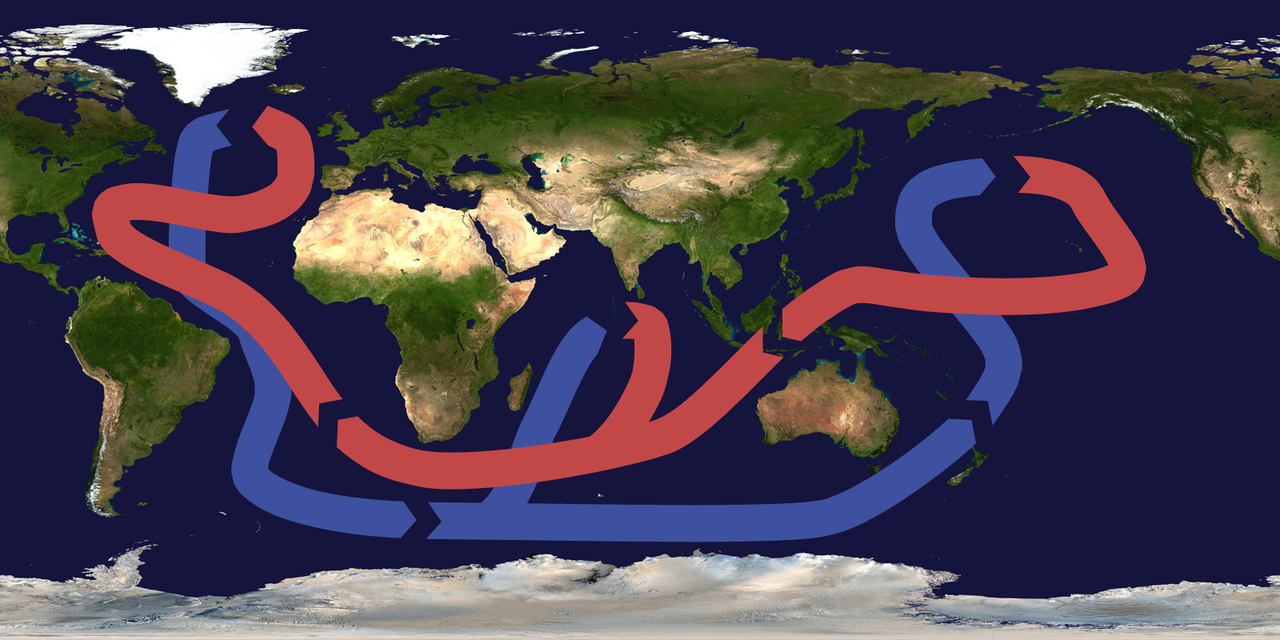
\includegraphics[width=\hsize]{chapters/4/1280px-Thermohaline_circulation.png}
\caption{
Das globale Förderband der thermohalinen Zirkulation.
\label{skript:thc:foerderband}}
\end{figure}%
Der Salzgehalt des Meerwassers ist nicht konstant,
hat aber ähnlich grossen Einfluss auf die Dichte wie die Temperatur.
Dies führt zu einer grossräumigen Zirkulationsströmung in den Weltmeeren,
genannt die thermohaline Zirkulation,
und damit zu einem weiteren bedeutenden Energietransportmechanismus.
Abbildung~\ref{skript:thc:foerderband} zeigt den Umfang der Zirkulation,
auch genannt das globale Förderband (conveyor belt).
Auf einer Zeitskala von Jahrzehnten bis Jahrhunderten wird Meerwasser 
und damit auch Wärmeenergie über Distanzen umgewälzt, welche mehrfach die
Erde umspannen.

Die Organismen, die in den oberen Wasserschichten absterben, sinken langsam
auf den Meeresgrund.
Ohne eine umfassende Umwälzung der Weltmeere würden die oberen Wasserschichten
mit der Zeit an Nährstoffen verarmen.
Die thermohaline Zirkulation stellt also auch die Versorgung der
Weltmeere mit Nährstoffen sicher.

Der Golfstrom ist ein kleiner Ausschnitt des globalen Förderbandes.
Die gut bekannte Bedeutung des Golfstroms für das europäische Klima 
deutet an, wie wichtig die thermohaline Zirkulation für das globale
Klima ist.
Es ist daher unerlässlich zu verstehen, was die Zirkulation antreibt und
wie sich der Klimawandel darauf auswirken könnte.

In diesem Kapitel soll die thermohaline Zirkulation modelliert werden.
Besonderes Augenmerk liegt dabei auf der Tatsache, dass dieses System
kippen kann.
Bei einer genügend grossen Änderung der Klimaparameter kann die Zirkulation
sich auf irreversible Art ändern.
Ein solches Ereignis hätte katastrophale Auswirkungen für das Klima.

\input{chapters/4/salinitaet.tex}
\input{chapters/4/schichtung.tex}
\input{chapters/4/box.tex}
\input{chapters/4/dimensionslos.tex}




%
% zonen.tex -- Zonenmodelle für das Klima
%
% (c) 2018 Prof Dr Andreas Müller, Hochschule Rapperswil
%
\chapter{Zonenmodelle\label{chapter:zonenmodelle}}
\lhead{Kapitel \thechapter: Zonenmodelle}
Die Erdrotation ist schnell im Vergleich zu den für typische Klimamodelle
wesentlichen Zeitspannen.
Wesentliche Aspekte der Klimaentwicklung sollten sich daher immer
noch modellieren lassen, wenn man den Zustand des Klimasystems über
die Erdrotation mittelt.
In diesem Kapitel werden daher vereinfachte Modelle diskutiert,
die nur die geographischen Länge als geometrischen Parameter haben.

\input{chapters/5/strahlung.tex}
\input{chapters/5/bilanz.tex}
\input{chapters/5/zonen.tex}
\input{chapters/5/spektral.tex}


%
% elnino.tex
%
% (c) 2018 Prof Dr Andreas Müller, Hochschule Rapperswil
%
\chapter{El Niño Southern Oscillation}
\lhead{El Niño Southern Oscillation}
Die Klimaentwicklung hängt wesentlich davon ab, wie Energie an der
Erdoberfläche verteilt wird.
Aus diesem Grund haben wir in Kapitel~\ref{chapter:fluiddynamik}
die Strömungsdynamik als den wesentlichen Mechanismus des 
Energietransportes in der Atmoshpäre studiert.
Und in Kapitel~\ref{chapter:thc} haben wir mit der Modellierung der
thermohalinen Zirkulation eine alternative Möglichkeit kennengelernt,
den Energie-Transport in den Weltmeeren zu beschreiben.

Das El Niño-Phänomen im Pazifik ist ein interessantes Teilsystem des
Klimasystems, welches einigermassen gut als isoliertes Teilsystem 
behandelt werden kann.
Die Modellierung, die wir in diesem Kapitel anstreben, braucht
einerseits die Ideen der Fluiddynamik, um die Energietransportmechanismen
zu beschreiben, und andererseits die Idee der Box-Modelle, um aus diesen
Mechanismen eine einfache gewöhnliche Differentiagleichung abzuleiten,
mit deren Hilfe die Dynamik des El~Niño studiert werden kann.

\section{El Niño}
\rhead{El Niño}

\input{chapters/7/kelvin.tex}
\input{chapters/7/rossby.tex}
\input{chapters/7/verzoegert.tex}


%
% assim.tex
%
% (c) 2018 Prof Dr Andreas Müller, Hochschule Rapperswil
%
\chapter{Datenassimilation}


\begin{appendices}
%\input{chapters/konstanten.tex}
%\input{chapters/komplexezahlen.tex}
\end{appendices}
\vfill
\pagebreak
\ifodd\value{page}\else\null\clearpage\fi
\lhead{Literatur}
\rhead{}
\printbibliography[heading=subbibliography]
\label{skript:literatur}
\end{refsection}

\part{Anwendungen und Weiterf"uhrende Themen}
\lhead{Anwendungen}
%
% uebersicht.tex -- Uebersicht ueber die Seminar-Arbeiten
%
% (c) 2018 Prof Dr Andreas Mueller, Hochschule Rapperswil
%
\chapter*{"Ubersicht}
\lhead{"Ubersicht}
\rhead{}
\label{skript:uebersicht}
Im zweiten Teil kommen die Teilnehmer des Seminars selbst zu Wort.
Die im ersten Teil dargelegten mathematischen Methoden und
grundlegenden Modelle werden dabei verfeinert, verallgemeinert
und auch numerisch überprüft.
Die Beispiele zeigen auch, dass umfassende Klimamodell erwartungsgemäss
schnell sehr komplex werden können.
Sie zeigen aber auch, dass es möglich ist, wesentliche Aspekte
des Klimas aus einfachen Überlegungen und mit übersichtlichen
mathematischen Modellen zu erfassen und zu verstehen.

{\em Matthias Baumann} und {\em Oliver Dias} zeigen zusätzliche
Informationen zum Lorenz-System, insbesondere zum Lorenz-Attraktor.
{\em Hansruedi Patzen} verallgemeinert das Vorgehen, mit dem das
Lorenz-System gewonnen wurde, im Sinne des Separationsverfahrens
für partielle Differentialgleichungen weiter, und gewinnt eine
Reihe von höherdimensionalen Lorenz-Systemen und untersucht weiter,
ob das beim dreidimensionalen System gefundene chaotische Verhalten 
auch in den höherdimensionalen Versionen zu finden ist.
Diese Untersuchungen zeigen, dass das Verhalten wahrscheinlich
nicht nur ein Artefakt der Reduktion auf drei Dimensionen ist, sondern
eine inhärente Eigenschaft des Lorenz-Systems.

Die exakte Lösung von Klimamodellen ist oft sehr schwierig, oft sind
Parameter oder Abhängigkeiten nicht bekannt.
Ein alternativer Ansatz ist daher, die zeitliche Entwicklung
im Sinne von machine learning zu lernen.
{\em Martin Stypinski} untersucht diesen Ansatz an zwei Beispielen,
der Wärmeleitungsgleichung und der nichtlinearen Gleichung von Burgers.
Die Beispiele zeigen vor allem auch, wie mathematisches Wissen über das
Modell hilft, die neuronalen Netzwerke zweckmässig zu entwerfen.

Die im Text entwickelten Modelle sind meist noch rudimentär, eine
reihe von Arbeiten haben sich daher mit Erweiterungen und Verfeinerungen
befasst.
{\em Jonas Gründler} hat das 2-Box Modell der thermohalinen Zirkulation
auf 3 Boxen verallgemeinert.
{\em Silvio Marti} studiert den Einfluss von Eis auf das Klima.
Die verzögerte Differentialgleichung des El Niño-Systems kann
numerische gelöst werden. {\em Raphael Unterer} zeigt, wie dies
funktioniert und findet insbesondere auch eine Stabilitätsbedingung
für sein Verfahren.
{\em Nicolas Tobler} hat versucht, die Modelle auf verschiedene
Planeten zu verallgemeinern und damit die Unterschiede der Atmosphären
der Planeten Venus, Erde und Mars zu erklären.
Die Einflüsse anderer Planeten zeigen sich zum Beispiel in der
Neigung der Erdachse gegen die Erdbahnebene.
Wie {\em Sebastian Lenhard} vorführt, können auch kleine Änderungen
der Neigung das Klima dramatisch verändern.
%Schliesslich gibt es auch eine Kopplung zwischen Klima und
%Vegetation, die {\em Matthias Dunkel} modelliert hat.

Die letzten zwei Kapitel befassen sich mit der Aufarbeitung der
Daten, auf grund derer wir zum Schluss kommen, dass 
der Klimawandel real ist.
Für Wetter- wie auch für Klimamodelle sind grosse Datenmengen
von Wetter- und Klimamessstationen in die Rechnung zu integrieren.
Der Kalman-Filter ist die Basis vieler moderner Lösungsansätze
für dieses Problem.
Am Beispiel des erweiterten Kalman-Filters für das Lorenz-System
zeigt {\em Michael Müller}, wie es möglich ist, den Systemzustand
selbst eines chaotischen nichtlinearen Systems zu 
Extreme Ereignisse sind in den letzten Jahren häufiger geworden
und werden oft als Indikatoren für die Klimaveränderung angeführt.
Wie man mit statistischen Daten über solche Ereignisse beweisen
kann, dass der Klimawandel tatsächlich stattfindet, zeigt
{\em Melina Staub}.






\def\chapterauthor#1{{\large #1}\bigskip\bigskip}
% Artikeverzoegert
%
% main.tex -- Paper zum Thema <thema>
%
% (c) 2018 Hochschule Rapperswil
%
\chapter{Achsneigung und Eiszeiten\label{chapter:thema}}
\lhead{Achseneigung und Eiszeiten}
\begin{refsection}
\chapterauthor{Sebastian Lenhard}

\section{Abschnitt}
\rhead{Abschnitt}

\section{Schlussfolgerung}
\rhead{Schlussfolgerung}

\printbibliography[heading=subbibliography]
\end{refsection}

%
% main.tex -- Paper zum Thema <thema>
%
% (c) 2018 Hochschule Rapperswil
%
\chapter{Achsneigung und Eiszeiten\label{chapter:thema}}
\lhead{Achseneigung und Eiszeiten}
\begin{refsection}
\chapterauthor{Sebastian Lenhard}

\section{Abschnitt}
\rhead{Abschnitt}

\section{Schlussfolgerung}
\rhead{Schlussfolgerung}

\printbibliography[heading=subbibliography]
\end{refsection}

%
% main.tex -- Paper zum Thema <thema>
%
% (c) 2018 Hochschule Rapperswil
%
\chapter{Achsneigung und Eiszeiten\label{chapter:thema}}
\lhead{Achseneigung und Eiszeiten}
\begin{refsection}
\chapterauthor{Sebastian Lenhard}

\section{Abschnitt}
\rhead{Abschnitt}

\section{Schlussfolgerung}
\rhead{Schlussfolgerung}

\printbibliography[heading=subbibliography]
\end{refsection}

%
% main.tex -- Paper zum Thema <thema>
%
% (c) 2018 Hochschule Rapperswil
%
\chapter{Achsneigung und Eiszeiten\label{chapter:thema}}
\lhead{Achseneigung und Eiszeiten}
\begin{refsection}
\chapterauthor{Sebastian Lenhard}

\section{Abschnitt}
\rhead{Abschnitt}

\section{Schlussfolgerung}
\rhead{Schlussfolgerung}

\printbibliography[heading=subbibliography]
\end{refsection}

%
% main.tex -- Paper zum Thema <thema>
%
% (c) 2018 Hochschule Rapperswil
%
\chapter{Achsneigung und Eiszeiten\label{chapter:thema}}
\lhead{Achseneigung und Eiszeiten}
\begin{refsection}
\chapterauthor{Sebastian Lenhard}

\section{Abschnitt}
\rhead{Abschnitt}

\section{Schlussfolgerung}
\rhead{Schlussfolgerung}

\printbibliography[heading=subbibliography]
\end{refsection}

%
% main.tex -- Paper zum Thema <thema>
%
% (c) 2018 Hochschule Rapperswil
%
\chapter{Achsneigung und Eiszeiten\label{chapter:thema}}
\lhead{Achseneigung und Eiszeiten}
\begin{refsection}
\chapterauthor{Sebastian Lenhard}

\section{Abschnitt}
\rhead{Abschnitt}

\section{Schlussfolgerung}
\rhead{Schlussfolgerung}

\printbibliography[heading=subbibliography]
\end{refsection}

%
% main.tex -- Paper zum Thema <thema>
%
% (c) 2018 Hochschule Rapperswil
%
\chapter{Achsneigung und Eiszeiten\label{chapter:thema}}
\lhead{Achseneigung und Eiszeiten}
\begin{refsection}
\chapterauthor{Sebastian Lenhard}

\section{Abschnitt}
\rhead{Abschnitt}

\section{Schlussfolgerung}
\rhead{Schlussfolgerung}

\printbibliography[heading=subbibliography]
\end{refsection}

%
% main.tex -- Paper zum Thema <thema>
%
% (c) 2018 Hochschule Rapperswil
%
\chapter{Achsneigung und Eiszeiten\label{chapter:thema}}
\lhead{Achseneigung und Eiszeiten}
\begin{refsection}
\chapterauthor{Sebastian Lenhard}

\section{Abschnitt}
\rhead{Abschnitt}

\section{Schlussfolgerung}
\rhead{Schlussfolgerung}

\printbibliography[heading=subbibliography]
\end{refsection}

%
% main.tex -- Paper zum Thema <thema>
%
% (c) 2018 Hochschule Rapperswil
%
\chapter{Achsneigung und Eiszeiten\label{chapter:thema}}
\lhead{Achseneigung und Eiszeiten}
\begin{refsection}
\chapterauthor{Sebastian Lenhard}

\section{Abschnitt}
\rhead{Abschnitt}

\section{Schlussfolgerung}
\rhead{Schlussfolgerung}

\printbibliography[heading=subbibliography]
\end{refsection}

%
% main.tex -- Paper zum Thema <thema>
%
% (c) 2018 Hochschule Rapperswil
%
\chapter{Achsneigung und Eiszeiten\label{chapter:thema}}
\lhead{Achseneigung und Eiszeiten}
\begin{refsection}
\chapterauthor{Sebastian Lenhard}

\section{Abschnitt}
\rhead{Abschnitt}

\section{Schlussfolgerung}
\rhead{Schlussfolgerung}

\printbibliography[heading=subbibliography]
\end{refsection}

%
% main.tex -- Paper zum Thema <thema>
%
% (c) 2018 Hochschule Rapperswil
%
\chapter{Achsneigung und Eiszeiten\label{chapter:thema}}
\lhead{Achseneigung und Eiszeiten}
\begin{refsection}
\chapterauthor{Sebastian Lenhard}

\section{Abschnitt}
\rhead{Abschnitt}

\section{Schlussfolgerung}
\rhead{Schlussfolgerung}

\printbibliography[heading=subbibliography]
\end{refsection}

\vfill
\pagebreak
\ifodd\value{page}\else\null\clearpage\fi
\lhead{Index}
\rhead{}
\addcontentsline{toc}{chapter}{\indexname}
%
% skript.tex -- Skript ueber Klimawandel
%
% (c) 2017 Prof. Dr. Andreas Mueller, HSR
%
\documentclass{book}
\usepackage{etex}
\usepackage{geometry}
\geometry{papersize={170mm,240mm},total={140mm,200mm},top=21mm,bindingoffset=10mm}
\usepackage[english,ngerman]{babel}
\usepackage[utf8]{inputenc}
\usepackage[T1]{fontenc}
\usepackage{cancel}
\usepackage{times}
\usepackage{amsmath,amscd}
\usepackage{amssymb}
\usepackage{amsfonts}
\usepackage{amsthm}
\usepackage{graphicx}
\usepackage{fancyhdr}
\usepackage{textcomp}
\usepackage{txfonts}
%\usepackage{alltt} 
\newcommand\hmmax{0}
\newcommand\bmmax{0}
\usepackage{bm}
\usepackage{verbatim}
\usepackage{paralist}
\usepackage{makeidx}
\usepackage{array}
%\usepackage[colorlinks=true]{hyperref}
\usepackage{hyperref}
\usepackage{tikz}
\usepackage{pgfplots}
\usepackage{pgfplotstable}
\usepackage{pdftexcmds}
\usepackage{pgfmath}
%\usepackage{placeins}
%\usepackage{subfigure}
\usepackage[autostyle=false,english=american]{csquotes}
%\usepackage{float}
%\usepackage{enumitem}
\usepackage{wasysym}
\usepackage{environ}
%\usepackage{pifont}
%\usepackage{feynmp}
\usepackage{appendix}
\usetikzlibrary{calc,intersections,through,backgrounds,graphs,positioning,shapes,arrows,fit}
\usetikzlibrary{patterns,decorations.pathreplacing}
\usetikzlibrary{decorations.pathreplacing}
\usetikzlibrary{external}
\usetikzlibrary{datavisualization}
\usepackage[europeanvoltages,
            europeancurrents,
            europeanresistors,   % rectangular shape
            americaninductors,   % "4-bumbs" shape
            europeanports,       % rectangular logic ports
            siunitx,             % #1<#2>
            emptydiodes,
            noarrowmos,
            smartlabels]         % lables are rotated in a smart way
           {circuitikz}          %
\usepackage{siunitx}
\usepackage{tabularx}
\usetikzlibrary{arrows}

\usepackage{algpseudocode}
\usepackage{algorithm}
\usepackage{gensymb}
\usepackage{mathtools}


% Matlab
\usepackage{listings}
\usepackage{color} %red, green, blue, yellow, cyan, magenta, black, white
\definecolor{mygreen}{RGB}{28,172,0} % color values Red, Green, Blue
\definecolor{mylilas}{RGB}{170,55,241}

\lstset{language=Matlab,%
    %basicstyle=\color{red},
    breaklines=true,%
    morekeywords={matlab2tikz},
    keywordstyle=\color{blue},%
    morekeywords=[2]{1}, keywordstyle=[2]{\color{black}},
    identifierstyle=\color{black},%
    stringstyle=\color{mylilas},
    commentstyle=\color{mygreen},%
    showstringspaces=false,%without this there will be a symbol in the places where there is a space
    numbers=left,%
    %numberstyle={\tiny \color{black}},% size of the numbers
    numbersep=9pt, % this defines how far the numbers are from the text
    emph=[1]{break},emphstyle=[1]\color{red}, %some words to emphasise
    %emph=[2]{word1,word2}, emphstyle=[2]{style},    
}
\lstdefinestyle{Matlab}{
  numbers=left,
  belowcaptionskip=1\baselineskip,
  breaklines=true,
  frame=L,
  xleftmargin=\parindent,
  language=Matlab,
  showstringspaces=false,
  basicstyle=\footnotesize\ttfamily,
  keywordstyle=\bfseries\color{green!40!black},
  commentstyle=\itshape\color{purple!40!black},
  identifierstyle=\color{blue},
  stringstyle=\color{orange},
  numberstyle=\ttfamily\tiny
}
\lstdefinelanguage{Matlab}{
  keywords={function,global,size,zeros,switch,case,otherwise,end,sin,cos,cot,floor,ode45,hold,polarplot},
  sensitive=true
}
\lstdefinelanguage{Maxima}{
  keywords={addrow,addcol,zeromatrix,ident,augcoefmatrix,ratsubst,sum,diff,ev,tex,%
    with_stdout,nouns,express,depends,load,length,submatrix,div,grad,curl,matrix,%
    invert,lambda,facsum,expand,false,then,if,else,subst,batchload,%
    rootscontract,solve,part,assume,sqrt,integrate,abs,inf,exp,sin,cos,sinh,cosh,taylor,ratsimp},
  sensitive=true,
  comment=[n][\itshape]{/*}{*/}
}
\lstdefinestyle{Maxima}{
  numbers=left,
  belowcaptionskip=1\baselineskip,
  breaklines=true,
  frame=L,
  xleftmargin=\parindent,
  language=Maxima,
  showstringspaces=false,
  basicstyle=\footnotesize\ttfamily,
  keywordstyle=\bfseries\color{green!40!black},
  commentstyle=\itshape\color{purple!40!black},
  identifierstyle=\color{blue},
  stringstyle=\color{orange},
  numberstyle=\ttfamily\tiny
}
\lstset{language=Octave,%
    %basicstyle=\color{red},
    breaklines=true,%
    morekeywords={function,global,size,zeros,switch,case,otherwise,end,sin,cos,cot,floor,ode45,hold,polarplot,endfunction,size,endswitch,cat,printf,for,endfor,if,return,endif,abs,while,endwhile},
    keywordstyle=\color{blue},%
    morekeywords=[2]{1}, keywordstyle=[2]{\color{black}},
    identifierstyle=\color{black},%
    stringstyle=\color{mylilas},
    commentstyle=\color{mygreen},%
    showstringspaces=false,%without this there will be a symbol in the places where there is a space
    numbers=left,%
    %numberstyle={\tiny \color{black}},% size of the numbers
    numbersep=9pt, % this defines how far the numbers are from the text
    emph=[1]{break},emphstyle=[1]\color{red}, %some words to emphasise
    %emph=[2]{word1,word2}, emphstyle=[2]{style},    
}
\lstdefinestyle{Octave}{
  numbers=left,
  belowcaptionskip=1\baselineskip,
  breaklines=true,
  frame=L,
  xleftmargin=\parindent,
  language=Octave,
  showstringspaces=false,
  basicstyle=\footnotesize\ttfamily,
  keywordstyle=\bfseries\color{green!40!black},
  commentstyle=\itshape\color{purple!40!black},
  identifierstyle=\color{blue},
  stringstyle=\color{orange},
  numberstyle=\ttfamily\tiny
}
\lstdefinestyle{C}{
  numbers=left,
  belowcaptionskip=1\baselineskip,
  breaklines=true,
  frame=L,
  xleftmargin=\parindent,
  language=C,
  showstringspaces=false,
  basicstyle=\footnotesize\ttfamily,
  keywordstyle=\bfseries\color{green!40!black},
  commentstyle=\itshape\color{purple!40!black},
  identifierstyle=\color{blue},
  stringstyle=\color{orange},
  numberstyle=\ttfamily\tiny
}
\usepackage{caption}
\usepackage[mode=buildnew]{standalone}
\usepackage[backend=bibtex]{biblatex}

% additional packages
%
% packages.tex -- zusätzliche Packages 
%
% In diesem File werden \usepackage{}-Aufrufe eingetragen für Packages, die
% noch nicht im skript.tex aufgerufen werden
%
% (c) 2018 Michael Müller, Hochschule Rapperswil
%


%
% packages.tex -- zusätzliche Packages 
%
% In diesem File werden \usepackage{}-Aufrufe eingetragen für Packages, die
% noch nicht im skript.tex aufgerufen werden
%
% (c) 2018 Michael Müller, Hochschule Rapperswil
%


%
% packages.tex -- zusätzliche Packages 
%
% In diesem File werden \usepackage{}-Aufrufe eingetragen für Packages, die
% noch nicht im skript.tex aufgerufen werden
%
% (c) 2018 Michael Müller, Hochschule Rapperswil
%


%
% packages.tex -- zusätzliche Packages 
%
% In diesem File werden \usepackage{}-Aufrufe eingetragen für Packages, die
% noch nicht im skript.tex aufgerufen werden
%
% (c) 2018 Michael Müller, Hochschule Rapperswil
%


%
% packages.tex -- zusätzliche Packages 
%
% In diesem File werden \usepackage{}-Aufrufe eingetragen für Packages, die
% noch nicht im skript.tex aufgerufen werden
%
% (c) 2018 Michael Müller, Hochschule Rapperswil
%


%
% packages.tex -- zusätzliche Packages 
%
% In diesem File werden \usepackage{}-Aufrufe eingetragen für Packages, die
% noch nicht im skript.tex aufgerufen werden
%
% (c) 2018 Michael Müller, Hochschule Rapperswil
%


%
% packages.tex -- zusätzliche Packages 
%
% In diesem File werden \usepackage{}-Aufrufe eingetragen für Packages, die
% noch nicht im skript.tex aufgerufen werden
%
% (c) 2018 Michael Müller, Hochschule Rapperswil
%


%
% packages.tex -- zusätzliche Packages 
%
% In diesem File werden \usepackage{}-Aufrufe eingetragen für Packages, die
% noch nicht im skript.tex aufgerufen werden
%
% (c) 2018 Michael Müller, Hochschule Rapperswil
%


%
% packages.tex -- zusätzliche Packages 
%
% In diesem File werden \usepackage{}-Aufrufe eingetragen für Packages, die
% noch nicht im skript.tex aufgerufen werden
%
% (c) 2018 Michael Müller, Hochschule Rapperswil
%


%
% packages.tex -- zusätzliche Packages 
%
% In diesem File werden \usepackage{}-Aufrufe eingetragen für Packages, die
% noch nicht im skript.tex aufgerufen werden
%
% (c) 2018 Michael Müller, Hochschule Rapperswil
%



% workaround for biblatex bug
\makeatletter
\def\blx@maxline{77}
\makeatother
\addbibresource{references.bib}
% Bibresources für jeden einzelnen Artikel
%\addbibresource{eis/references.bib}
%\addbibresource{extrem/references.bib}
%\addbibresource{kalman/references.bib}
%\addbibresource{learning/references.bib}
\addbibresource{lorenz/references.bib}
%\addbibresource{lorenz2/references.bib}
%\addbibresource{planeten/references.bib}
%\addbibresource{thermohalin/references.bib}
%\addbibresource{vegetation/references.bib}
%\addbibresource{verzoegert/references.bib}
\AtEndDocument{\clearpage\ifodd\value{page}\else\null\clearpage\fi}
\makeindex
%\pgfplotsset{compat=1.12}
\setlength{\headheight}{15pt} % fix headheight warning
\DeclareGraphicsRule{*}{mps}{*}{}
\begin{document}
\pagestyle{fancy}
\frontmatter
\newcommand\HRule{\noindent\rule{\linewidth}{1.5pt}}
\begin{titlepage}
\vspace*{\stretch{1}}
\HRule
\vspace*{5pt}
\begin{flushright}
{
\LARGE
Mathematisches Seminar\\
\vspace*{20pt}
\Huge
Klimawandel%
}
\vspace*{5pt}
\end{flushright}
\HRule
\begin{flushright}
\vspace{60pt}
\Large
Leitung: Andreas M"uller\\
\vspace{40pt}
\Large
%
% teilnehmer.tex -- Liste der Seminarteilnehmer für Titelseite
%
% (c) 2018 Prof Dr Andreas Müller, Hochschule Rapperswil
%
Matthias Baumann,
Oliver Dias-Lalcaca,
%Matthias Dunkel%,
Jonas Gründler%,
\\
Sebastian Lenhard,
Silvio Marti,
Michael~Müller,
Hansruedi~Patzen%,
\\
Melina~Staub,
Martin~Stypinski,
Nicolas Tobler,
Raphael Unterer
\\

%Matthias Baumann,
%Oliver Dias-Lalcaca,
%Matthias Dunkel%,
%\\
%Flurina Hoby,
%Sebastian Lenhard,
%Silvio Marti,
%Hansruedi~Patzen%,
%\\
%Melina~Staub,
%Martin~Stypinski,
%Nicolas Tobler,
%Raphael Unterer
\end{flushright}
\vspace*{\stretch{2}}
\begin{center}
Hochschule f"ur Technik, Rapperswil, 2018
\end{center}
\end{titlepage}
\hypersetup{
    linktoc=all,
    linkcolor=blue
}
\newcounter{beispiel}
\newenvironment{beispiele}{
\bgroup\smallskip\parindent0pt\bf Beispiele\egroup

\begin{list}{\arabic{beispiel}.}
  {\usecounter{beispiel}
  \setlength{\labelsep}{5mm}
  \setlength{\rightmargin}{0pt}
}}{\end{list}}
\newcounter{uebungsaufgabezaehler}
% environment fuer uebungsaufgaben
\newenvironment{uebungsaufgaben}{
\begin{list}{\arabic{uebungsaufgabezaehler}.}
  {\usecounter{uebungsaufgabezaehler}
  \setlength{\labelwidth}{2cm}
  \setlength{\leftmargin}{0pt}
  \setlength{\labelsep}{5mm}
  \setlength{\rightmargin}{0pt}
  \setlength{\itemindent}{0pt}
}}{\end{list}\vfill\pagebreak}
\newenvironment{teilaufgaben}{
\begin{enumerate}
\renewcommand{\labelenumi}{\alph{enumi})}
}{\end{enumerate}}
% Aufgabe
\newcounter{problemcounter}[chapter]
\def\aufgabenpath{chapters/uebungsaufgaben/}
\def\ainput#1{\input\aufgabenpath/#1}
\def\verbatimainput#1{\expandafter\verbatiminput{\aufgabenpath/#1}}
\def\aufgabetoplevel#1{%
\expandafter\def\expandafter\inputpath{#1}%
\let\aufgabepath=\inputpath
}
\def\includeagraphics[#1]#2{\expandafter\includegraphics[#1]{\aufgabepath#2}}
% \aufgabe
\newcommand{\uebungsaufgabe}[1]{%
\refstepcounter{problemcounter}%
\label{#1}%
\bigskip{\parindent0pt\strut}\hbox{\bf\arabic{problemcounter}. }%
\expandafter\def\csname aufgabenpath\endcsname{\inputpath/}%
\expandafter\input{chapters/uebungsaufgaben/#1.tex}
}
\renewcommand\theproblemcounter{\thechapter.\arabic{problemcounter}}

% Loesung
\def\swallow#1{
%nothing
}
\NewEnviron{loesung}[1][L"osung]{%
\begin{proof}[#1]%
\renewcommand{\qedsymbol}{$\bigcirc$}
\BODY
\end{proof}
}
\NewEnviron{bewertung}{%
\begin{proof}[Bewertung]%
\renewcommand{\qedsymbol}{}
\BODY
\end{proof}
}
\NewEnviron{diskussion}{%
\begin{proof}[Diskussion]%
\renewcommand{\qedsymbol}{}
\BODY
\end{proof}
}
\NewEnviron{hinweis}{%
\begin{proof}[Hinweis]%
\renewcommand{\qedsymbol}{}
\BODY
\end{proof}
}
\def\keineloesungen{%
\RenewEnviron{loesung}{\relax}
\RenewEnviron{bewertung}{\relax}
\RenewEnviron{diskussion}{\relax}
}
\newenvironment{beispiel}{%
\begin{proof}[Beispiel]%
\renewcommand{\qedsymbol}{$\bigcirc$}
}{\end{proof}}

\allowdisplaybreaks

\lhead{Inhaltsverzeichnis}
\rhead{}
\tableofcontents
\newtheorem{satz}{Satz}[chapter]
\newtheorem{hilfssatz}[satz]{Hilfssatz}
\newtheorem{definition}[satz]{Definition}
\newtheorem{annahme}[satz]{Annahme}
\newtheorem{problem}[satz]{Problem}
\newtheorem*{problem*}{Problem}
\renewcommand{\floatpagefraction}{0.7}
\mainmatter
%
% vorwort.tex -- Vorwort zum Buch zum Seminar
%
% (c) 2017 Prof Dr Andreas Mueller, Hochschule Rapperswil
%
\chapter*{Vorwort}
\lhead{Vorwort}
\rhead{}
Dieses Buch entstand im Rahmen des Mathematischen Seminars
im Frühjahrssemester 2017 an der Hochschule für Technik Rapperswil.
Die Teilnehmer, Studierende der Abteilungen für Elektrotechnik,
Informatik und Bauingenieurwesen der
HSR, erarbeiteten nach einer Einführung in das Themengebiet jeweils
einzelne Aspekte des Gebietes in Form einer Seminararbeit, über
deren Resultate sie auch in einem Vortrag informierten. 

Im Frühjahr 2018 war das Thema des Seminars der Klimawandel.

Im zweiten Teil dieses Skripts kommen dann die Teilnehmer selbst zu Wort.
Ihre Arbeiten wurden jeweils als einzelne
Kapitel mit meist nur typographischen Änderungen übernommen.
Diese weiterführenden Kapitel sind sehr verschiedenartig.
Eine Übersicht und Einführung findet sich in der Einleitung
zum zweiten Teil auf Seite~\pageref{skript:uebersicht}.

In einigen Arbeiten wurde auch Code zur Demonstration der 
besprochenen Methoden und Resultate geschrieben, soweit
möglich und sinnvoll wurde dieser Code im Github-Repository
dieses Kurses%
\footnote{\url{https://github.com/AndreasFMueller/SeminarKlima.git}}
abgelegt.

Im genannten Repository findet sich auch der Source-Code dieses
Skriptes, es wird hier unter einer Creative Commons Lizenz
zur Verfügung gestellt.
Auf der beiliegenden DVD befinden sich die Testdaten und Programme
zu zwei der simulationsintensiveren Artikel im zweiten Teil.



\part{Grundlagen}
%\keineloesungen
\begin{refsection}
%
% part1.tex
%
% (c) 2018 Prof Dr Andreas Müller, Hochschule Rapperswil
%
\input{chapters/wuk.tex}
\input{chapters/dgl.tex}
\input{chapters/thc.tex}
\input{chapters/zonen.tex}
\input{chapters/elnino.tex}
\input{chapters/assim.tex}

\begin{appendices}
%\input{chapters/konstanten.tex}
%\input{chapters/komplexezahlen.tex}
\end{appendices}
\vfill
\pagebreak
\ifodd\value{page}\else\null\clearpage\fi
\lhead{Literatur}
\rhead{}
\printbibliography[heading=subbibliography]
\label{skript:literatur}
\end{refsection}

\part{Anwendungen und Weiterf"uhrende Themen}
\lhead{Anwendungen}
%
% uebersicht.tex -- Uebersicht ueber die Seminar-Arbeiten
%
% (c) 2018 Prof Dr Andreas Mueller, Hochschule Rapperswil
%
\chapter*{"Ubersicht}
\lhead{"Ubersicht}
\rhead{}
\label{skript:uebersicht}
Im zweiten Teil kommen die Teilnehmer des Seminars selbst zu Wort.
Die im ersten Teil dargelegten mathematischen Methoden und
grundlegenden Modelle werden dabei verfeinert, verallgemeinert
und auch numerisch überprüft.
Die Beispiele zeigen auch, dass umfassende Klimamodell erwartungsgemäss
schnell sehr komplex werden können.
Sie zeigen aber auch, dass es möglich ist, wesentliche Aspekte
des Klimas aus einfachen Überlegungen und mit übersichtlichen
mathematischen Modellen zu erfassen und zu verstehen.

{\em Matthias Baumann} und {\em Oliver Dias} zeigen zusätzliche
Informationen zum Lorenz-System, insbesondere zum Lorenz-Attraktor.
{\em Hansruedi Patzen} verallgemeinert das Vorgehen, mit dem das
Lorenz-System gewonnen wurde, im Sinne des Separationsverfahrens
für partielle Differentialgleichungen weiter, und gewinnt eine
Reihe von höherdimensionalen Lorenz-Systemen und untersucht weiter,
ob das beim dreidimensionalen System gefundene chaotische Verhalten 
auch in den höherdimensionalen Versionen zu finden ist.
Diese Untersuchungen zeigen, dass das Verhalten wahrscheinlich
nicht nur ein Artefakt der Reduktion auf drei Dimensionen ist, sondern
eine inhärente Eigenschaft des Lorenz-Systems.

Die exakte Lösung von Klimamodellen ist oft sehr schwierig, oft sind
Parameter oder Abhängigkeiten nicht bekannt.
Ein alternativer Ansatz ist daher, die zeitliche Entwicklung
im Sinne von machine learning zu lernen.
{\em Martin Stypinski} untersucht diesen Ansatz an zwei Beispielen,
der Wärmeleitungsgleichung und der nichtlinearen Gleichung von Burgers.
Die Beispiele zeigen vor allem auch, wie mathematisches Wissen über das
Modell hilft, die neuronalen Netzwerke zweckmässig zu entwerfen.

Die im Text entwickelten Modelle sind meist noch rudimentär, eine
reihe von Arbeiten haben sich daher mit Erweiterungen und Verfeinerungen
befasst.
{\em Jonas Gründler} hat das 2-Box Modell der thermohalinen Zirkulation
auf 3 Boxen verallgemeinert.
{\em Silvio Marti} studiert den Einfluss von Eis auf das Klima.
Die verzögerte Differentialgleichung des El Niño-Systems kann
numerische gelöst werden. {\em Raphael Unterer} zeigt, wie dies
funktioniert und findet insbesondere auch eine Stabilitätsbedingung
für sein Verfahren.
{\em Nicolas Tobler} hat versucht, die Modelle auf verschiedene
Planeten zu verallgemeinern und damit die Unterschiede der Atmosphären
der Planeten Venus, Erde und Mars zu erklären.
Die Einflüsse anderer Planeten zeigen sich zum Beispiel in der
Neigung der Erdachse gegen die Erdbahnebene.
Wie {\em Sebastian Lenhard} vorführt, können auch kleine Änderungen
der Neigung das Klima dramatisch verändern.
%Schliesslich gibt es auch eine Kopplung zwischen Klima und
%Vegetation, die {\em Matthias Dunkel} modelliert hat.

Die letzten zwei Kapitel befassen sich mit der Aufarbeitung der
Daten, auf grund derer wir zum Schluss kommen, dass 
der Klimawandel real ist.
Für Wetter- wie auch für Klimamodelle sind grosse Datenmengen
von Wetter- und Klimamessstationen in die Rechnung zu integrieren.
Der Kalman-Filter ist die Basis vieler moderner Lösungsansätze
für dieses Problem.
Am Beispiel des erweiterten Kalman-Filters für das Lorenz-System
zeigt {\em Michael Müller}, wie es möglich ist, den Systemzustand
selbst eines chaotischen nichtlinearen Systems zu 
Extreme Ereignisse sind in den letzten Jahren häufiger geworden
und werden oft als Indikatoren für die Klimaveränderung angeführt.
Wie man mit statistischen Daten über solche Ereignisse beweisen
kann, dass der Klimawandel tatsächlich stattfindet, zeigt
{\em Melina Staub}.






\def\chapterauthor#1{{\large #1}\bigskip\bigskip}
% Artikeverzoegert
%
% main.tex -- Paper zum Thema <thema>
%
% (c) 2018 Hochschule Rapperswil
%
\chapter{Achsneigung und Eiszeiten\label{chapter:thema}}
\lhead{Achseneigung und Eiszeiten}
\begin{refsection}
\chapterauthor{Sebastian Lenhard}

\section{Abschnitt}
\rhead{Abschnitt}

\section{Schlussfolgerung}
\rhead{Schlussfolgerung}

\printbibliography[heading=subbibliography]
\end{refsection}

%
% main.tex -- Paper zum Thema <thema>
%
% (c) 2018 Hochschule Rapperswil
%
\chapter{Achsneigung und Eiszeiten\label{chapter:thema}}
\lhead{Achseneigung und Eiszeiten}
\begin{refsection}
\chapterauthor{Sebastian Lenhard}

\section{Abschnitt}
\rhead{Abschnitt}

\section{Schlussfolgerung}
\rhead{Schlussfolgerung}

\printbibliography[heading=subbibliography]
\end{refsection}

%
% main.tex -- Paper zum Thema <thema>
%
% (c) 2018 Hochschule Rapperswil
%
\chapter{Achsneigung und Eiszeiten\label{chapter:thema}}
\lhead{Achseneigung und Eiszeiten}
\begin{refsection}
\chapterauthor{Sebastian Lenhard}

\section{Abschnitt}
\rhead{Abschnitt}

\section{Schlussfolgerung}
\rhead{Schlussfolgerung}

\printbibliography[heading=subbibliography]
\end{refsection}

%
% main.tex -- Paper zum Thema <thema>
%
% (c) 2018 Hochschule Rapperswil
%
\chapter{Achsneigung und Eiszeiten\label{chapter:thema}}
\lhead{Achseneigung und Eiszeiten}
\begin{refsection}
\chapterauthor{Sebastian Lenhard}

\section{Abschnitt}
\rhead{Abschnitt}

\section{Schlussfolgerung}
\rhead{Schlussfolgerung}

\printbibliography[heading=subbibliography]
\end{refsection}

%
% main.tex -- Paper zum Thema <thema>
%
% (c) 2018 Hochschule Rapperswil
%
\chapter{Achsneigung und Eiszeiten\label{chapter:thema}}
\lhead{Achseneigung und Eiszeiten}
\begin{refsection}
\chapterauthor{Sebastian Lenhard}

\section{Abschnitt}
\rhead{Abschnitt}

\section{Schlussfolgerung}
\rhead{Schlussfolgerung}

\printbibliography[heading=subbibliography]
\end{refsection}

%
% main.tex -- Paper zum Thema <thema>
%
% (c) 2018 Hochschule Rapperswil
%
\chapter{Achsneigung und Eiszeiten\label{chapter:thema}}
\lhead{Achseneigung und Eiszeiten}
\begin{refsection}
\chapterauthor{Sebastian Lenhard}

\section{Abschnitt}
\rhead{Abschnitt}

\section{Schlussfolgerung}
\rhead{Schlussfolgerung}

\printbibliography[heading=subbibliography]
\end{refsection}

%
% main.tex -- Paper zum Thema <thema>
%
% (c) 2018 Hochschule Rapperswil
%
\chapter{Achsneigung und Eiszeiten\label{chapter:thema}}
\lhead{Achseneigung und Eiszeiten}
\begin{refsection}
\chapterauthor{Sebastian Lenhard}

\section{Abschnitt}
\rhead{Abschnitt}

\section{Schlussfolgerung}
\rhead{Schlussfolgerung}

\printbibliography[heading=subbibliography]
\end{refsection}

%
% main.tex -- Paper zum Thema <thema>
%
% (c) 2018 Hochschule Rapperswil
%
\chapter{Achsneigung und Eiszeiten\label{chapter:thema}}
\lhead{Achseneigung und Eiszeiten}
\begin{refsection}
\chapterauthor{Sebastian Lenhard}

\section{Abschnitt}
\rhead{Abschnitt}

\section{Schlussfolgerung}
\rhead{Schlussfolgerung}

\printbibliography[heading=subbibliography]
\end{refsection}

%
% main.tex -- Paper zum Thema <thema>
%
% (c) 2018 Hochschule Rapperswil
%
\chapter{Achsneigung und Eiszeiten\label{chapter:thema}}
\lhead{Achseneigung und Eiszeiten}
\begin{refsection}
\chapterauthor{Sebastian Lenhard}

\section{Abschnitt}
\rhead{Abschnitt}

\section{Schlussfolgerung}
\rhead{Schlussfolgerung}

\printbibliography[heading=subbibliography]
\end{refsection}

%
% main.tex -- Paper zum Thema <thema>
%
% (c) 2018 Hochschule Rapperswil
%
\chapter{Achsneigung und Eiszeiten\label{chapter:thema}}
\lhead{Achseneigung und Eiszeiten}
\begin{refsection}
\chapterauthor{Sebastian Lenhard}

\section{Abschnitt}
\rhead{Abschnitt}

\section{Schlussfolgerung}
\rhead{Schlussfolgerung}

\printbibliography[heading=subbibliography]
\end{refsection}

%
% main.tex -- Paper zum Thema <thema>
%
% (c) 2018 Hochschule Rapperswil
%
\chapter{Achsneigung und Eiszeiten\label{chapter:thema}}
\lhead{Achseneigung und Eiszeiten}
\begin{refsection}
\chapterauthor{Sebastian Lenhard}

\section{Abschnitt}
\rhead{Abschnitt}

\section{Schlussfolgerung}
\rhead{Schlussfolgerung}

\printbibliography[heading=subbibliography]
\end{refsection}

\vfill
\pagebreak
\ifodd\value{page}\else\null\clearpage\fi
\lhead{Index}
\rhead{}
\addcontentsline{toc}{chapter}{\indexname}
%
% skript.tex -- Skript ueber Klimawandel
%
% (c) 2017 Prof. Dr. Andreas Mueller, HSR
%
\documentclass{book}
\usepackage{etex}
\usepackage{geometry}
\geometry{papersize={170mm,240mm},total={140mm,200mm},top=21mm,bindingoffset=10mm}
\usepackage[english,ngerman]{babel}
\usepackage[utf8]{inputenc}
\usepackage[T1]{fontenc}
\usepackage{cancel}
\usepackage{times}
\usepackage{amsmath,amscd}
\usepackage{amssymb}
\usepackage{amsfonts}
\usepackage{amsthm}
\usepackage{graphicx}
\usepackage{fancyhdr}
\usepackage{textcomp}
\usepackage{txfonts}
%\usepackage{alltt} 
\newcommand\hmmax{0}
\newcommand\bmmax{0}
\usepackage{bm}
\usepackage{verbatim}
\usepackage{paralist}
\usepackage{makeidx}
\usepackage{array}
%\usepackage[colorlinks=true]{hyperref}
\usepackage{hyperref}
\usepackage{tikz}
\usepackage{pgfplots}
\usepackage{pgfplotstable}
\usepackage{pdftexcmds}
\usepackage{pgfmath}
%\usepackage{placeins}
%\usepackage{subfigure}
\usepackage[autostyle=false,english=american]{csquotes}
%\usepackage{float}
%\usepackage{enumitem}
\usepackage{wasysym}
\usepackage{environ}
%\usepackage{pifont}
%\usepackage{feynmp}
\usepackage{appendix}
\usetikzlibrary{calc,intersections,through,backgrounds,graphs,positioning,shapes,arrows,fit}
\usetikzlibrary{patterns,decorations.pathreplacing}
\usetikzlibrary{decorations.pathreplacing}
\usetikzlibrary{external}
\usetikzlibrary{datavisualization}
\usepackage[europeanvoltages,
            europeancurrents,
            europeanresistors,   % rectangular shape
            americaninductors,   % "4-bumbs" shape
            europeanports,       % rectangular logic ports
            siunitx,             % #1<#2>
            emptydiodes,
            noarrowmos,
            smartlabels]         % lables are rotated in a smart way
           {circuitikz}          %
\usepackage{siunitx}
\usepackage{tabularx}
\usetikzlibrary{arrows}

\usepackage{algpseudocode}
\usepackage{algorithm}
\usepackage{gensymb}
\usepackage{mathtools}


% Matlab
\usepackage{listings}
\usepackage{color} %red, green, blue, yellow, cyan, magenta, black, white
\definecolor{mygreen}{RGB}{28,172,0} % color values Red, Green, Blue
\definecolor{mylilas}{RGB}{170,55,241}

\lstset{language=Matlab,%
    %basicstyle=\color{red},
    breaklines=true,%
    morekeywords={matlab2tikz},
    keywordstyle=\color{blue},%
    morekeywords=[2]{1}, keywordstyle=[2]{\color{black}},
    identifierstyle=\color{black},%
    stringstyle=\color{mylilas},
    commentstyle=\color{mygreen},%
    showstringspaces=false,%without this there will be a symbol in the places where there is a space
    numbers=left,%
    %numberstyle={\tiny \color{black}},% size of the numbers
    numbersep=9pt, % this defines how far the numbers are from the text
    emph=[1]{break},emphstyle=[1]\color{red}, %some words to emphasise
    %emph=[2]{word1,word2}, emphstyle=[2]{style},    
}
\lstdefinestyle{Matlab}{
  numbers=left,
  belowcaptionskip=1\baselineskip,
  breaklines=true,
  frame=L,
  xleftmargin=\parindent,
  language=Matlab,
  showstringspaces=false,
  basicstyle=\footnotesize\ttfamily,
  keywordstyle=\bfseries\color{green!40!black},
  commentstyle=\itshape\color{purple!40!black},
  identifierstyle=\color{blue},
  stringstyle=\color{orange},
  numberstyle=\ttfamily\tiny
}
\lstdefinelanguage{Matlab}{
  keywords={function,global,size,zeros,switch,case,otherwise,end,sin,cos,cot,floor,ode45,hold,polarplot},
  sensitive=true
}
\lstdefinelanguage{Maxima}{
  keywords={addrow,addcol,zeromatrix,ident,augcoefmatrix,ratsubst,sum,diff,ev,tex,%
    with_stdout,nouns,express,depends,load,length,submatrix,div,grad,curl,matrix,%
    invert,lambda,facsum,expand,false,then,if,else,subst,batchload,%
    rootscontract,solve,part,assume,sqrt,integrate,abs,inf,exp,sin,cos,sinh,cosh,taylor,ratsimp},
  sensitive=true,
  comment=[n][\itshape]{/*}{*/}
}
\lstdefinestyle{Maxima}{
  numbers=left,
  belowcaptionskip=1\baselineskip,
  breaklines=true,
  frame=L,
  xleftmargin=\parindent,
  language=Maxima,
  showstringspaces=false,
  basicstyle=\footnotesize\ttfamily,
  keywordstyle=\bfseries\color{green!40!black},
  commentstyle=\itshape\color{purple!40!black},
  identifierstyle=\color{blue},
  stringstyle=\color{orange},
  numberstyle=\ttfamily\tiny
}
\lstset{language=Octave,%
    %basicstyle=\color{red},
    breaklines=true,%
    morekeywords={function,global,size,zeros,switch,case,otherwise,end,sin,cos,cot,floor,ode45,hold,polarplot,endfunction,size,endswitch,cat,printf,for,endfor,if,return,endif,abs,while,endwhile},
    keywordstyle=\color{blue},%
    morekeywords=[2]{1}, keywordstyle=[2]{\color{black}},
    identifierstyle=\color{black},%
    stringstyle=\color{mylilas},
    commentstyle=\color{mygreen},%
    showstringspaces=false,%without this there will be a symbol in the places where there is a space
    numbers=left,%
    %numberstyle={\tiny \color{black}},% size of the numbers
    numbersep=9pt, % this defines how far the numbers are from the text
    emph=[1]{break},emphstyle=[1]\color{red}, %some words to emphasise
    %emph=[2]{word1,word2}, emphstyle=[2]{style},    
}
\lstdefinestyle{Octave}{
  numbers=left,
  belowcaptionskip=1\baselineskip,
  breaklines=true,
  frame=L,
  xleftmargin=\parindent,
  language=Octave,
  showstringspaces=false,
  basicstyle=\footnotesize\ttfamily,
  keywordstyle=\bfseries\color{green!40!black},
  commentstyle=\itshape\color{purple!40!black},
  identifierstyle=\color{blue},
  stringstyle=\color{orange},
  numberstyle=\ttfamily\tiny
}
\lstdefinestyle{C}{
  numbers=left,
  belowcaptionskip=1\baselineskip,
  breaklines=true,
  frame=L,
  xleftmargin=\parindent,
  language=C,
  showstringspaces=false,
  basicstyle=\footnotesize\ttfamily,
  keywordstyle=\bfseries\color{green!40!black},
  commentstyle=\itshape\color{purple!40!black},
  identifierstyle=\color{blue},
  stringstyle=\color{orange},
  numberstyle=\ttfamily\tiny
}
\usepackage{caption}
\usepackage[mode=buildnew]{standalone}
\usepackage[backend=bibtex]{biblatex}

% additional packages
\input{eis/packages.tex}
\input{extrem/packages.tex}
\input{kalman/packages.tex}
\input{learning/packages.tex}
\input{lorenz/packages.tex}
\input{lorenz2/packages.tex}
\input{planeten/packages.tex}
\input{thermohalin/packages.tex}
\input{vegetation/packages.tex}
\input{verzoegert/packages.tex}

% workaround for biblatex bug
\makeatletter
\def\blx@maxline{77}
\makeatother
\addbibresource{references.bib}
% Bibresources für jeden einzelnen Artikel
%\addbibresource{eis/references.bib}
%\addbibresource{extrem/references.bib}
%\addbibresource{kalman/references.bib}
%\addbibresource{learning/references.bib}
\addbibresource{lorenz/references.bib}
%\addbibresource{lorenz2/references.bib}
%\addbibresource{planeten/references.bib}
%\addbibresource{thermohalin/references.bib}
%\addbibresource{vegetation/references.bib}
%\addbibresource{verzoegert/references.bib}
\AtEndDocument{\clearpage\ifodd\value{page}\else\null\clearpage\fi}
\makeindex
%\pgfplotsset{compat=1.12}
\setlength{\headheight}{15pt} % fix headheight warning
\DeclareGraphicsRule{*}{mps}{*}{}
\begin{document}
\pagestyle{fancy}
\frontmatter
\newcommand\HRule{\noindent\rule{\linewidth}{1.5pt}}
\begin{titlepage}
\vspace*{\stretch{1}}
\HRule
\vspace*{5pt}
\begin{flushright}
{
\LARGE
Mathematisches Seminar\\
\vspace*{20pt}
\Huge
Klimawandel%
}
\vspace*{5pt}
\end{flushright}
\HRule
\begin{flushright}
\vspace{60pt}
\Large
Leitung: Andreas M"uller\\
\vspace{40pt}
\Large
\input{teilnehmer.tex}
%Matthias Baumann,
%Oliver Dias-Lalcaca,
%Matthias Dunkel%,
%\\
%Flurina Hoby,
%Sebastian Lenhard,
%Silvio Marti,
%Hansruedi~Patzen%,
%\\
%Melina~Staub,
%Martin~Stypinski,
%Nicolas Tobler,
%Raphael Unterer
\end{flushright}
\vspace*{\stretch{2}}
\begin{center}
Hochschule f"ur Technik, Rapperswil, 2018
\end{center}
\end{titlepage}
\hypersetup{
    linktoc=all,
    linkcolor=blue
}
\newcounter{beispiel}
\newenvironment{beispiele}{
\bgroup\smallskip\parindent0pt\bf Beispiele\egroup

\begin{list}{\arabic{beispiel}.}
  {\usecounter{beispiel}
  \setlength{\labelsep}{5mm}
  \setlength{\rightmargin}{0pt}
}}{\end{list}}
\newcounter{uebungsaufgabezaehler}
% environment fuer uebungsaufgaben
\newenvironment{uebungsaufgaben}{
\begin{list}{\arabic{uebungsaufgabezaehler}.}
  {\usecounter{uebungsaufgabezaehler}
  \setlength{\labelwidth}{2cm}
  \setlength{\leftmargin}{0pt}
  \setlength{\labelsep}{5mm}
  \setlength{\rightmargin}{0pt}
  \setlength{\itemindent}{0pt}
}}{\end{list}\vfill\pagebreak}
\newenvironment{teilaufgaben}{
\begin{enumerate}
\renewcommand{\labelenumi}{\alph{enumi})}
}{\end{enumerate}}
% Aufgabe
\newcounter{problemcounter}[chapter]
\def\aufgabenpath{chapters/uebungsaufgaben/}
\def\ainput#1{\input\aufgabenpath/#1}
\def\verbatimainput#1{\expandafter\verbatiminput{\aufgabenpath/#1}}
\def\aufgabetoplevel#1{%
\expandafter\def\expandafter\inputpath{#1}%
\let\aufgabepath=\inputpath
}
\def\includeagraphics[#1]#2{\expandafter\includegraphics[#1]{\aufgabepath#2}}
% \aufgabe
\newcommand{\uebungsaufgabe}[1]{%
\refstepcounter{problemcounter}%
\label{#1}%
\bigskip{\parindent0pt\strut}\hbox{\bf\arabic{problemcounter}. }%
\expandafter\def\csname aufgabenpath\endcsname{\inputpath/}%
\expandafter\input{chapters/uebungsaufgaben/#1.tex}
}
\renewcommand\theproblemcounter{\thechapter.\arabic{problemcounter}}

% Loesung
\def\swallow#1{
%nothing
}
\NewEnviron{loesung}[1][L"osung]{%
\begin{proof}[#1]%
\renewcommand{\qedsymbol}{$\bigcirc$}
\BODY
\end{proof}
}
\NewEnviron{bewertung}{%
\begin{proof}[Bewertung]%
\renewcommand{\qedsymbol}{}
\BODY
\end{proof}
}
\NewEnviron{diskussion}{%
\begin{proof}[Diskussion]%
\renewcommand{\qedsymbol}{}
\BODY
\end{proof}
}
\NewEnviron{hinweis}{%
\begin{proof}[Hinweis]%
\renewcommand{\qedsymbol}{}
\BODY
\end{proof}
}
\def\keineloesungen{%
\RenewEnviron{loesung}{\relax}
\RenewEnviron{bewertung}{\relax}
\RenewEnviron{diskussion}{\relax}
}
\newenvironment{beispiel}{%
\begin{proof}[Beispiel]%
\renewcommand{\qedsymbol}{$\bigcirc$}
}{\end{proof}}

\allowdisplaybreaks

\lhead{Inhaltsverzeichnis}
\rhead{}
\tableofcontents
\newtheorem{satz}{Satz}[chapter]
\newtheorem{hilfssatz}[satz]{Hilfssatz}
\newtheorem{definition}[satz]{Definition}
\newtheorem{annahme}[satz]{Annahme}
\newtheorem{problem}[satz]{Problem}
\newtheorem*{problem*}{Problem}
\renewcommand{\floatpagefraction}{0.7}
\mainmatter
\input{vorwort.tex}
\part{Grundlagen}
%\keineloesungen
\begin{refsection}
\input{chapters/part1.tex}
\begin{appendices}
%\input{chapters/konstanten.tex}
%\input{chapters/komplexezahlen.tex}
\end{appendices}
\vfill
\pagebreak
\ifodd\value{page}\else\null\clearpage\fi
\lhead{Literatur}
\rhead{}
\printbibliography[heading=subbibliography]
\label{skript:literatur}
\end{refsection}

\part{Anwendungen und Weiterf"uhrende Themen}
\lhead{Anwendungen}
\input{uebersicht.tex}
\def\chapterauthor#1{{\large #1}\bigskip\bigskip}
% Artikeverzoegert
\input{eis/main.tex}
\input{extrem/main.tex}
\input{kalman/main.tex}
\input{learning/main.tex}
\input{lorenz/main.tex}
\input{lorenz2/main.tex}
\input{neigung/main.tex}
\input{planeten/main.tex}
\input{thermohalin/main.tex}
\input{vegetation/main.tex}
\input{verzoegert/main.tex}
\vfill
\pagebreak
\ifodd\value{page}\else\null\clearpage\fi
\lhead{Index}
\rhead{}
\addcontentsline{toc}{chapter}{\indexname}
\input{skript.ind}

\end{document}


\end{document}


\end{document}


\end{document}
